%% 
%% Copyright 2007, 2008, 2009 Elsevier Ltd
%% 
%% This file is part of the 'Elsarticle Bundle'.
%% ---------------------------------------------
%% 
%% It may be distributed under the conditions of the LaTeX Project Public
%% License, either version 1.2 of this license or (at your option) any
%% later version.  The latest version of this license is in
%%    http://www.latex-project.org/lppl.txt
%% and version 1.2 or later is part of all distributions of LaTeX
%% version 1999/12/01 or later.
%% 
%% The list of all files belonging to the 'Elsarticle Bundle' is
%% given in the file `manifest.txt'.
%% 

%% Template article for Elsevier's document class `elsarticle'
%% with numbered style bibliographic references
%% SP 2008/03/01

\documentclass[final,5p,twocolumn]{elsarticle}

%% Use the option review to obtain double line spacing
%% \documentclass[authoryear,preprint,review,12pt]{elsarticle}

%% Use the options 1p,twocolumn; 3p; 3p,twocolumn; 5p; or 5p,twocolumn
%% for a journal layout:
%% \documentclass[final,1p,times]{elsarticle}
%% \documentclass[final,1p,times,twocolumn]{elsarticle}
%% \documentclass[final,3p,times]{elsarticle}
%% \documentclass[final,3p,times,twocolumn]{elsarticle}
%% \documentclass[final,5p,times]{elsarticle}
%% \documentclass[final,5p,times,twocolumn]{elsarticle}

%% For including figures, graphicx.sty has been loaded in
%% elsarticle.cls. If you prefer to use the old commands
%% please give \usepackage{epsfig}

%% The amssymb package provides various useful mathematical symbols
\usepackage{amssymb}
\usepackage{mathtools, amssymb}
\usepackage{xspace}
\usepackage{verbatim}
\usepackage[usenames]{color}
\usepackage[usenames,dvipsnames,table]{xcolor}
\usepackage{url}
\usepackage{array}
\usepackage{color}
\usepackage{longtable}
\usepackage{wrapfig}
\usepackage{tikz}
\usetikzlibrary{graphs}
\usetikzlibrary{backgrounds}
\usepackage{subcaption}
\usepackage[hidelinks]{hyperref}

    
% \usepackage[pdftex,dvips]{graphicx}

\DeclareMathOperator*{\argmin}{argmin}
\newcommand{\mat}[1]{\ensuremath{\begin{bmatrix}#1\end{bmatrix}}}	% matrix
\newcommand{\Rv}[1]{{\mathbb{R}^{#1}}}				% set of real-valued vectors
\newcommand{\R}[2]{{\mathbb{R}^{#1\times #2}}}		% set of real-valued matrices


%% The amsthm package provides extended theorem environments
%% \usepackage{amsthm}

%% The lineno packages adds line numbers. Start line numbering with
%% \begin{linenumbers}, end it with \end{linenumbers}. Or switch it on
%% for the whole article with \linenumbers.
%% \usepackage{lineno}

%% \journal{Nuclear Physics B}

\begin{document}

\begin{frontmatter}

%% Title, authors and addresses

%% use the tnoteref command within \title for footnotes;
%% use the tnotetext command for theassociated footnote;
%% use the fnref command within \author or \address for footnotes;
%% use the fntext command for theassociated footnote;
%% use the corref command within \author for corresponding author footnotes;
%% use the cortext command for theassociated footnote;
%% use the ead command for the email address,
%% and the form \ead[url] for the home page:
%% \title{Title\tnoteref{label1}}
%% \tnotetext[label1]{}
%% \author{Name\corref{cor1}\fnref{label2}}
%% \ead{email address}
%% \ead[url]{home page}
%% \fntext[label2]{}
%% \cortext[cor1]{}
%% \address{Address\fnref{label3}}
%% \fntext[label3]{}

\title{Whole-body multi-contact motion in Humans and Humanoids:\\mid-term advances of the CoDyCo european project}

%% use optional labels to link authors explicitly to addresses:
%% \author[label1,label2]{}
%% \address[label1]{}
%% \address[label2]{}

\author{Vincent Padois}
\address{Sorbonne Universit\'{e}s, UPMC Univ Paris 06, UMR 7222, Institut des Syst\`{e}mes Intelligents et de Robotique, Paris, France.\\CNRS, UMR 7222, Institut des Syst\`{e}mes Intelligents et de Robotique, Paris, France. Email: vincent.padois@upmc.fr}

\author{Serena Ivaldi}
\address{Inria, Villers-l\`{e}s-Nancy, France.\\
CNRS  \& Universit\'e de Lorraine, UMR 7503, Loria, Vandoeuvre-l\`{e}s-Nancy, France. Email: serena.ivaldi@inria.fr}

\author{Jan Babi\v{c}}
\address{Jo\v{z}ef Stefan Institute, Ljubljana, Slovenia. Email: jan.babic@ijs.si}

\author{Michael Mistry }
\address{University of Birmingham, Birmingham, United Kingdom. Email: m.n.mistry@bham.ac.uk}

\author{Jan Peters}
\address{Max Planck Institute for Intelligent Systems and TU Darmstadt, Darmstadt, Germany. Email: mail@jan-peters.net}

\author{Francesco Nori}
\address{Robotics, Brain and Cognitive Science Department, Istituto Italiano di Tecnologia, Genova, Italy. Email: francesco.nori@iit.it}


\begin{abstract}
Traditional industrial applications involve robots with limited mobility. Consequently, interaction (\textit{e.g.} manipulation) was treated separately from whole-body posture (\textit{e.g.} balancing), assuming the robot firmly connected to the ground. Foreseen applications involve robots with augmented autonomy and physical mobility. Within this novel context, physical interaction influences stability and balance. To allow robots to surpass barriers between interaction and posture control, forthcoming robotic research needs to investigate the principles governing whole-body motion and coordination with contact dynamics. There is a need to investigate the principles of motion and coordination of physical interaction, including the aspects related to unpredictability. Recent developments in compliant actuation and touch sensing allow safe and robust physical interaction from unexpected contact including humans. The next advancement for cognitive robots, however, is the ability not only to cope with unpredictable contact, but also to exploit predictable contact in ways that will assist in goal achievement. Last but not least, theoretical results needs to be validated in real-world scenarios with humanoid robots engaged in whole-body goal-directed tasks. Robots should be capable of exploiting rigid supportive contacts, learning to compensate for compliant contacts, and utilising assistive physical interaction from humans. The work presented in this paper presents state-of-the-art in these domains as well as some recent advances made within the framework of the CoDyCo european project.
\end{abstract}

\begin{keyword}
whole-body \sep control \sep free-floating \sep interaction \sep contacts \sep compliance.
%% keywords here, in the form: keyword  keyword

%% PACS codes here, in the form: \PACS code \sep code

%% MSC codes here, in the form: \MSC code \sep code
%% or \MSC[2008] code \sep code (2000 is the default)

\end{keyword}

\end{frontmatter}

%% \linenumbers

%% main text
\section{Introduction}
\label{sec:intro}

For cognitive agents, such as humanoid robots, to persist and act in natural human environments, contact and physical interaction become necessary and unavoidable. Everyday tasks involve making and breaking contact, among all areas of the body, whether the contacts are accidental disturbances or intentional support for dynamic movement. Critically, robots should be robust enough to cope with unpredictable contact, via safe control mechanisms and compliance.  Moreover, cognitive goal directed robots need the ability to exploit predictable contact, to aid in goal achievement, as well as learn dynamics of contact in order to generalise to novel tasks and domains.

Physical interaction has been studied in robotics, extensively under the umbrella of manipulation. For historical reasons, these studies have assumed a fixed-base as cur-rent industrial applications do not necessitate extended mobility. Foreseen robotic applications will demand an increasing level of autonomy, including physical mobility. These applications call for extending studies on interaction to cases where the robot has a mobile-base. Remarkably and differently from the fixed-base case, interaction in these situations may compromise system balance, and goal directed actions require proper whole-body coordination and use of contact. However, the principles governing whole-body coordination in humans are far from being understood and implementations on complex systems, such as humanoids, are missing, especially besides walking.

Within this context one of the major challenges of robotic research is to advance the current control and cognitive understanding about robust, goal-directed whole-body motion execution with multiple contacts. Remarkably, focus should be posed on complex systems, such as humans and humanoids. In a crescendo of complexity, as illustrated in Figure~\ref{fig:scenarios}, the current state-of-the-art in these domains (state-of-art 1 and 2) should be advanced to address more complex scenarios (challenges 1 and 2).

\paragraph{State-of-art 1: balancing with multiple rigid contacts} The robot is standing and balancing with its hands supported by a rigid table in front of its body. However, the table is unstable, and unexpectedly the contact with the table breaks. A contact state change is sensed, and the robot's control architecture automatically adjusts posture control parameters to maintain balance in light of the reduced support. The unexpected breaking of contact makes it more challenging.

\paragraph{State-of-art 2: goal directed actions involving contacts} The robot is standing with its hands at its side, and intends to reach for an object on a table in front.  The robot recognises that the distance is sufficiently far away, and the task cannot be achieved without compromising balance.  The robot decides to initiate a new contact with its left hand on the table, providing sufficient support for reaching the object with its right hand.

\paragraph{Challenge 1: learning non-rigid contacts} The robot sits down on a chair with a soft cushion, however the cushion has a particular stiffness quality not experienced before. The robot tries to reach for an object on a table, but it fails as it did not adequately compensate for the unexpected dynamics of the soft cushion. After a few attempts, the robot adapts its model of the contact interaction, and is able to infer new control action to successfully reach the goal.

\paragraph{Challenge 2: human assistive contacts} The robot is seated in a chair, and a person comes to assist the robot to stand. He/she grabs both hands of the robot and starts pulling upwards.  The robot senses the new contact, and recognising from the interaction force that it is an external agent, allows its arms to be compliant.  When the force becomes sufficient to enable standing, the robot recognises the intended action and stiffens its arms while pushing its legs to rise from the chair. Finally once standing, but still in contact with the human, the robot returns compliance to its arms to allow for safe interaction while retaining overall control of its posture.

\begin{figure}
\centering
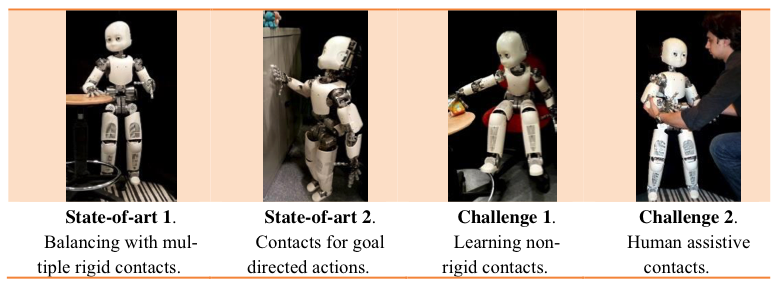
\includegraphics[width=1.0\linewidth]{./images/scenarios.png}
%\label{fig:subfig2}
\caption{The four main scenarios involving whole-body motion with multiple contacts, addressed in the CoDyCo project.}
\label{fig:scenarios}
\end{figure}

\subsection {Compliance in whole-body motion}

Present day robots are still far from the human capabilities in exploiting predictable events and in coping with uncertainty. The gap between humans and robots is particularly apparent when in tasks involving unstructured physical interaction with the environment or other agents. Recent behavioural experiments yielded a new perspective on modelling the way humans deal with both predictable and unpredictable motor control tasks. In early experiments, it has been shown \cite{Shadmehr1994a} that humans learn and adapt internal dynamical models of their own arm in interaction with the environment. Such internal models appear to be crucial in predicting how muscle activations produce hand movements and therefore may play an essential predictive role in movement planning. However, Burdet et al. \cite{Burdet2001} have shown that when prediction is not a viable strategy, humans can rely on arm compliance regulation (by means of muscle co-activation) to cope with the unpredictability that naturally arises from feedback delays when performing arm-reaching movements in unstable environments. Basic research and robotics technology are ready to extend such insights from single limb movements to whole-body interaction and the validation of these models appears feasible. In contrast to manipulation scenarios with static base robot systems, dynamic whole-body interaction concerns the analysis of phenomena at a higher scale (bigger interaction forces, bigger muscle activations, etc.).  Whole-body compliance regulation with force/impedance control is not only favoured by current theoretical progress and available technologies, but may actually be ready for widespread use instead of being limited to just a few prototypes.

\begin{figure}
\centering
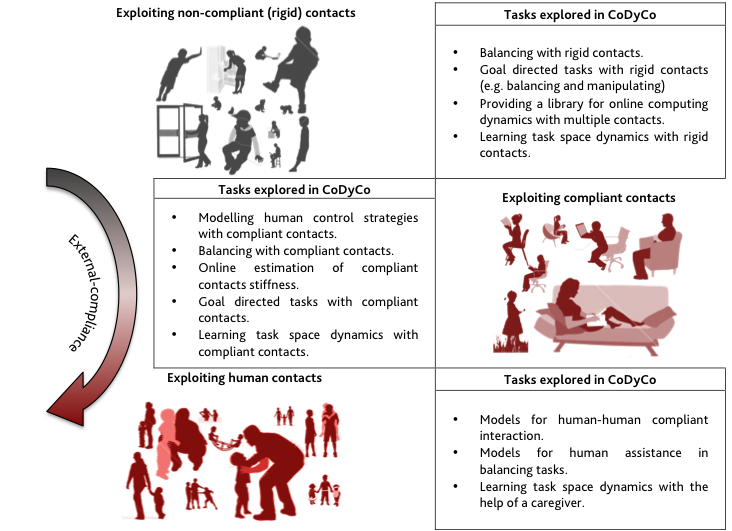
\includegraphics[width=\linewidth]{./images/classification1.png}
%\label{fig:subfig2}
\caption{Classification of whole-body tasks based on external-compliance. The complexity increases from top to bottom, \textit{i.e.}, with the need of exploiting the compliance of the contacts.}
\label{fig:classification1}
\end{figure}

\subsection{Roadmap beyond state-of-the-art}

With reference to Figure~\ref{fig:classification1} and following, we propose a classification that relies on the well known concept of compliance (or the inverse concept of stiffness and more generally impedance), to be understood as the force-displacement characteristic of a contact. Interaction scenarios can be classified by quantitatively measuring two essential components of contacts: external and internal compliance (internal here refers to the agent or ``the self''). The first scenarios classification (Figure~\ref{fig:classification1}) is based on the external-compliance; it includes scenarios that involve non-compliant (rigid) external contacts and scenarios with compliant external contacts. This second category is extremely wide in consideration of the multitude of possible compliant behaviours that can be experienced: from the linear force-displacement characteristic of a linear spring to the complex non-linear characteristic of a pillow. Scenarios within this category practically overlap with the first category but rigid contacts are replaced by non-rigid contacts. In these two categories the agent (or ``the self'', represented with a human silhouette) is always interacting with inanimate objects (the external contacts: a chair, a sofa, the floor, etc.). In the last category, ``the self'' and ``the other'' are both humans. In these scenarios the external-compliance is not a well-defined relationship between force and displacement but depends on the active intention of ``the other''.

External-compliance is only one side of the interaction, and the agent has limited control over it. The other side of the interaction is what we call the ``self'' (internal) compliance, which is instead fully under control of the cognitive agent. Self-compliance needs to be adapted to the environment compliance and the ability to actively regulate the internal compliance has been only recently implemented on multi-degrees-of-freedom robots. The self-compliance regulation represents the pro-active and cognitive component of the interaction and therefore gives the robot an enhanced degree of autonomy to be exploited in handling situations not anticipated at design time. In this sense, the self-compliance level and actuation range can be used to classify different scenarios as shown by Figure~\ref{fig:classification2}. At the very first level of this classification we consider scenarios that do not require significant self-compliance regulation as they typically involve dynamically stable situations. Such situations involve for example dynamically stable tasks, which substantially require direct control of stable postures. The second level of the classification includes tasks that require a certain level of active compliance either to stabilise unstable systems (\textit{e.g.} balancing) or to compensate for unpredictable interaction characteristics (\textit{e.g.} standing hand in hand with another agent). Finally at the highest level of this classification we consider highly complex tasks characterised by strong requirements in terms of ``self''-compliance planning and regulation.

\begin{figure}
\centering
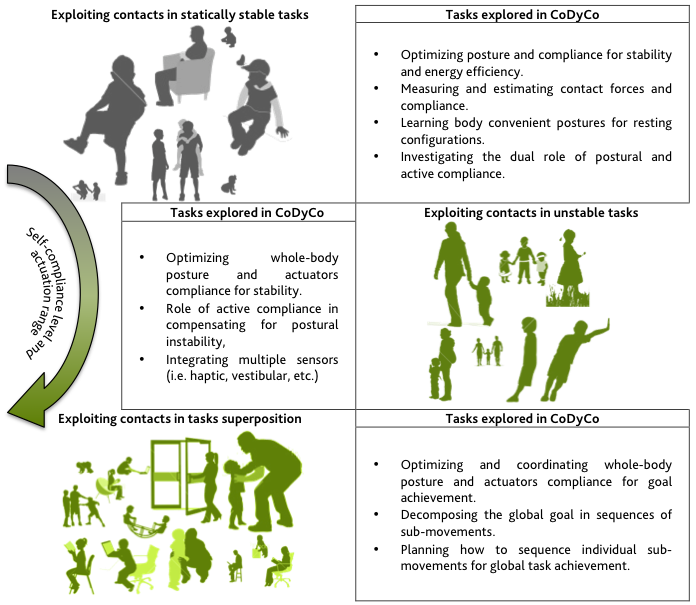
\includegraphics[width=\linewidth]{./images/classification2.png}
%\label{fig:subfig2}
\caption{Classification of whole-body tasks according to an increasing self-compliance level and actuation range.}
\label{fig:classification2}
\end{figure}

External and self-compliance are two fundamental aspects of any interaction. It is therefore crucial to understand how these two concepts become intertwined once contacts are established. The concept of contact-compliance indeed corresponds to the overall compliance obtained once the external and the self-compliance become coupled with the contact establishment. A contact can be seen as the serial connection of two compliances, one representing the external-compliance, the other representing the self-compliance. The compliance of a serial interconnection is simply the linear sum of the individual compliances. Roughly speaking, the contact-compliance does not significantly change when the external and self-compliance are changed simultaneously by an equal and opposite quantity. No advancement can be associated to situations which correspond to augmenting the self-compliance at the cost of diminishing the external-compliance or vice versa, as in these situations the overall contact-compliance does not change. This fundamental procedural principle is well sketched in Figure~\ref{fig:classification3}. The horizontal axis sorts possible scenarios according to a progressively increasing external-compliance level. The vertical axis instead orders the same scenarios by means of increasing self-compliance levels and actuation ranges: tasks involving minimal self-compliance regulation or low levels of compliance are shown at the bottom; tasks involving wide self-compliance regulation ranges including high compliance levels are at the top. The grey-colour-valued function shown in the space defined by these two axes is a qualitative evaluation of progress beyond the state-of-the-art: dark grey is the state-of-the-art, increasing levels of blue represent step-by-step progress beyond state-of-the-art. Progress in handling whole body contacts can be achieved only by simultaneously increasing the external and the self-compliance levels. Conversely, little advances are achieved when increasing the environmental compliance but reducing the active compliance component. Vice versa, a dual way to achieve little progress beyond the state-of-the-art corresponds to scenarios that involve a strong self-compliance regulation but reduced external-compliance.  

\begin{figure}[!ht]
\centering
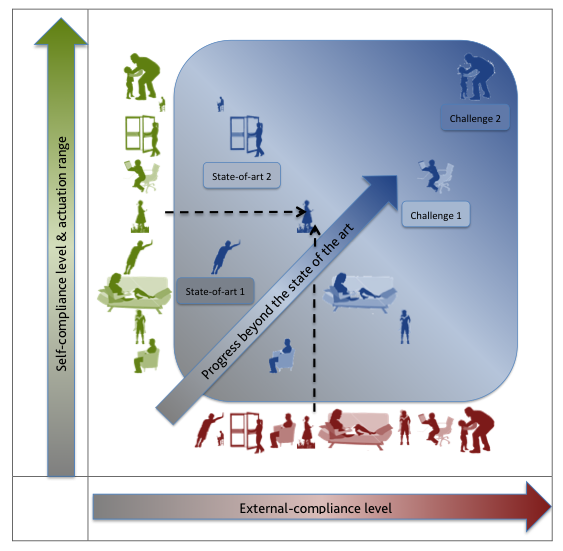
\includegraphics[width=\linewidth]{./images/classification3.png}
\caption{The metric space to evaluate the progress work beyond the current state-of-the-art. Interaction is the inter-twined combination of two components, external and self-compliance, both contributing to the concept of contact-compliance. Whole-body scenarios should be evaluated in a metric space that takes into account how self and external-compliance contribute to contact-compliance. Contact-compliance is the sum of self and external-compliance. Remarkably the major advances can be obtained by simultaneously advancing the external and the self-compliance requirements. The vertical axis represents both self-compliance levels and actuation ranges in consideration of the fact we are mainly interested in self-compliance regulation, actuation and control. The four proposed scenarios have increasing complexity with respect to current state-of-the-art. }
\label{fig:classification3}
\end{figure}


\subsection{Scope of the paper}

Looking at whole-body multi-contact motion in Humans and Humanoids through the prism of external and self compliance, and more generally contact compliance, provides an original and insightful light to the addressed question. It is a good starting point to define the problems to be addressed in this domain. These problems can be divided in four closely intertwined domains: control theory, machine learning, human behavioural experiments and software development. Each of them serve the objectives of the CoDyCo project:
\begin{enumerate}
\item develop a general software toolkit for whole-body dynamics computation with multiple external contacts;
\item conduct human behavioural studies for understanding human use of external contact with environments exhibiting different external compliances\footnote{and more generally \textit{impedances}.}, including interpersonal cooperative contacts in natural whole body tasks;
\item develop a control architecture for whole-body coordination and regulation of whole body compliance;
\item leverage machine learning methods for acquiring models of compliant contact with the environment and physical interactions with humans and provide the humanoid robot control architecture with the core abilities for the adaptation, generalization and self-improvement of both control laws and tasks related to these types of physical interaction.
\end{enumerate}

In these domains, numerous technological and scientific developments have been led over the last decades. A brief overview of these related works is provided in the next section. The strength of the CoDyCo approach with respect to some of these existing works is to gather expertises in different fields around a very challenging scientific question. Interesting synergies between these different domains are much more likely to  emerge in these conditions. The following sections are directly related to three scientific domains mentioned here-before and describe the work led within the framework of the CoDyCo project in human postural control and whole-body motion in contact with the environment, whole-body controllers and learning respectively. Future works are described in the conclusion which also summarizes the major findings of the project.

\section{State-of-the-art}

In this section, a brief overview of some of the key aspects in the state-of-the-art related to whole-body motion in contact for humans and humanoids are presented.

\subsection{Technological state-of-the-art}
Among the recent achievements in the field of robotics, there are two major technological prerequisites that will play a fundamental role in enhancing whole-body motion capabilities: distributed force and touch sensing. Both technologies have been only recently integrated and used in (humanoid) robots, including the iCub \cite{MettaG._etal2010}.
Force control is a fundamental property for any autonomous agent in interaction with the environment. First attempts to regulate interaction forces relied on active force and compliance control schemes, typically coupled with custom mechanical designs such as the ones proposed in \cite{Salisbury1988} and \cite{Hayashi2007}, which were eventually implemented on successful commercial manipulators. Similar solutions have been eventually implemented on some humanoid platforms \cite{Cheng2006} \cite{Escande2010}, including the iCub \cite{Fumagalli2012}. Recent theoretical and technological advances have revealed the importance of intentionally introducing mechanical compliance in the design \cite{Pratt1995} and (even more recently) the necessity of actively regulating the actuator passive compliance \cite{Koganezawa2005} \cite{Tonietti2005} \cite{Migliore2005}. It is to be expected that within the next years robots such as iCub will be equipped with variably compliant actuation technologies at some (if not all) of the main joints \cite{Tsagarakis2009} \cite{Tsagarakis2011}.

Touch is another fundamental sensing capability for autonomous agents willing to interact with an unstructured environment or humans \cite{Argall2010a}. Whole-body distributed touch sensing has been only recently embedded on humanoid robots, but there already exist quite a few examples: Robovie-IV \cite{Mitsunaga2006}, RI-MAN \cite{Mukai2008}, Macra \cite{Hayashi2007}  and Meka \cite{Jain}, just to cite a few. The iCub already integrates a mature technology \cite{Schmitz2011} covering the upper body, legs and feet soles. 
Finally, several open-source software libraries have been developed in the last years to support research in whole-body dynamics and contact simulation. Several dynamics simulators have been developed for robotics (see \cite{ivaldi2014} for a survey). The most interesting physics engines for our purposes are the ones with Featherstone-like forward dynamics calculation \cite{Featherstone2008} \cite{Yamane2006a}, built-in collision detection and stable numerical contact forces computations \cite{Nakaoka2007}. Among the kinematic and dynamic libraries it is worth citing HuMAnS, a toolbox for analysis and control of both human and humanoid motion, and iDyn, a generic software library for computation of whole-body dynamics and external contact forces of complex manipulators and humanoids \cite{Ivaldi2011}. iDyn has been extensively used in iCub to compute whole-body dynamics as it enables to reinforce these computations with measurements coming from inertial, force and tactile sensors embedded in the robot \cite{Fumagalli2012}.

\subsection{Human motor control state-of-the-art}
Human whole-body motion control has been studied within tasks such as reaching on a supporting surface and sit-to-stand. These movements involve coordination of multiple joints, significant shift of the centre of mass, and control of equilibrium, either in static or dynamic conditions. These are skills learnt early in human childhood but also studied extensively in the context of motor disability, \textit{e.g.} after neurological insults like stroke, or in the elderly with reduced muscle power, joint flexibility and sensory loss. However, almost nothing is yet known about when healthy subjects choose to make use of contacts with support surfaces. It has been shown that in standing posture, this contact provides augmented sensory information reducing sway \cite{Johannsen2012}, and how in some circumstances, non-weight bearing but informative ``light-touch'' between two standing subjects can cause coupling that leads to increased sway, emphasising that knowledge about the stability and compliance of the contact surface is vital.

\paragraph{Reach using supports}
Human reaching with arm support has not been extensively studied. There is almost no literature on the issue of how humans use one hand to extend their reach space. For example, to lean forwards requires a shift of the trunk and a shift of the centre of mass \cite{Huang2011}. At some point it becomes advantageous to use a supporting surface, allowing a reduction in anticipatory postural adjustments and a simplified control strategy \cite{Slijper2000}. But the decisions about when to implement support using one arm, which will depend on the availability, reliability and compliance of a support surface are almost unstudied \cite{Krishnamoorthy2004}.

\paragraph{Sit-to-stand} The postural adjustments that contribute to a sit-to-stand action are well documented. The action requires a shift of centre of mass, development of momentum, and precisely timed hip and knee extension, combining with maintaining stability with ankle control. As motor ability lessens, \textit{e.g.} in the elderly, compensatory foot placement with increased momentum generation using hip flexion and arm movement is often employed \cite{Janssen2002}. Support from the chair arm or from a cane \cite{Leung2009}  increases stability in the forward axis. Again, decisions about when the support surface would be used, depending on its stability and compliance, are unstudied. The effects of unstable foot support in the sit-to-stand action are studied in \cite{Huang2011} the authors suggests a clear trade-off between support surface stability and manoeuvrability, and argue that adapting to the added uncertainty could help individuals become more manoeuvrable. Finally, there is little work on how the sit-to-stand action changes with elastic support - this has been studied in locomotion and jumping \cite{Arampatzis2001}, but not in inter-actions with support surfaces.

\paragraph{Dimensionality reduction}
Complex multi-joint movements call for control strategies that simplify and reduce degrees of freedom. There are various competing theories of how this can be achieved \cite{Latash2010}. Perhaps most relevant is the uncontrolled manifold hypothesis \cite{Scholz1999} that demonstrates that it is highly effective to allow some parameters to be uncontrolled, if task irrelevant, and to control only a fewer task relevant parameters. In \cite{Scholz1999} Scholz \& Schoner applied this to the sit-to-stand task, and show that the centre of mass in the forward axis is well controlled, head and hand position are less controlled, and vertical head position appears little controlled. How these behaviours change with support is an open question. Equally important is the issue of how high dimensionality whole body motion of human models can be reduced to extract principles of action applicable to robots with different geometries. These are implemented by muscle and joint synergies that reduce the functional degrees of freedom during a given action. There has been very effective use of principal or independent components analyses to capture such human whole body movement and reduce dimensionality (\textit{e.g.} as in \cite{Forner-Cordero2005}). Recent developments include extracting functional components, which treat joint-kinematics data as functions instead of as a series of independent samples, and are comparable across groups of subjects \cite{Coffey2011}.

\subsection{Robot control state-of-the-art}
In complex scenarios, when the robot and the environment are assumed to be perfectly known, planning approaches explore the possible states of the robot (\textit{e.g.} configurations of the robot in its environment) in probabilistic graph-like manners \cite{LaValle2006} to determine the sequence of commands to provide to the robot to perform a certain action in free space \cite{Dalibard2009} \cite{Kuffner2001} or in complex contact situations \cite{Bouyarmane2009} \cite{Bouyarmane2011}. Such methods are usually computationally demanding and difficult to apply online. Conversely, when the global goal of the robot is relatively simple, the high-level planner can be almost disregarded because the goal to be achieved can ``easily'' be described \textit{a priori} in terms of operational tasks \cite{Khatib1986} to be activated and combined. This falls into ``the simultaneous management of multiple operational objectives'', a well-known problem in model-based reactive control. The most popular method to deal with a set of objectives is a hierarchical framework, where operational tasks are typically prioritized in a ``stack'' \cite{Mansard2007}, which found several applications to humanoids \cite{Sentis2010} \cite{Mistry2011}. QP (Quadratic Program) solvers have recently gained popularity in humanoid robotics as they do not require the explicit inversion of any model of the system \cite{abe2007} \cite{colette2008} \cite{Escande2010} \cite{Salini2011}. This corpus of reactive methods mostly succeeds in over-coming the ``complexity and uncertainty'' factor thanks to the use of feedback. However the proposed solutions are only locally optimal and the overall decision-making process cannot be addressed in the most general cases (\textit{i.e.} without scripted scenarios). There is obviously a need for approaches where planning and reactive control are combined in a strongly intertwined way. This is not a simple problem: there are very few works where such a combination has actually been tested in a non ad hoc manner. The work of \cite{Alami1997} contributed to describe the necessary control architecture but did not propose any general control solution for such a combination to exist in practice. More recently \cite{PhilippsenRolandandNejatiNeginandSentis2009} introduced an architecture combining a whole body control level and a reactive symbolic planning, while \cite{yoshida2005} focused on dedicated mission-level planning methods for humanoids, coupled to task-level controllers. \cite{Salini2011} \cite{salini2011b} have also proposed an architecture where sequences of operational tasks are generated on the fly based on a fuzzy-logic, rule-based decision engine. This approach, even though efficient in various specific applications, fails to scale-up as the number of required rules explodes with the growing complexity of the considered scenarios.

\subsection{Learning}
Real-world environments are often hard to capture perfectly with physical models. The uncertainty in model predictions is important during controlled physical contacts between a (humanoid) robot system and its environment. Large errors either in the environmental model or in the task will lead to drastic failures and therefore need to be limited as much as possible by model adaptation. Human-inhabited worlds will never allow perfect modelling and instead require that the system generalises the tasks in such a manner that they work in a wide variety of different uncertain scenarios where there is contact between robots and either humans or physical objects. Machine learning approaches are therefore needed. Particularly in whole-body motion they are necessary for the successful implementation of the control architecture, and its implementation and application to the real-worlds scenarios. However, off-the-shelf machine learning methods are concerned with static data sets and require massive amount of computations, often rendering real-time learning in-feasible. To date, a variety of robot learning approaches have been suggested. The most important being model learning, operational space control learning, learning of elementary tasks and hierarchical combinations of tasks, which are briefly evaluated hereinafter.

\paragraph{Model learning}
 High model accuracy and constant model adaptation may be key for low torque interaction during contact. Models of the robot dynamics have been learned by real-time regression, \textit{e.g.}, locally weighted projection regression \cite{Schaal2002a} and local Gaussian process regression \cite{Nguyen-tuong2010a}. Learning force/torque models in iCub has been investigated with different regression techniques, such as SVM and Neural Networks \cite{Fumagalli2010learning}. Nevertheless, if any of these approaches would be given the data from a robot in contact with the environment, it would fit the model to this particular case, as the contact forces would just be treated as an additional non-linearity. As a result, the model will not generalise to new contact models and instead it would be necessary to learn a new model for each type of contact.

\paragraph{Operational space control learning}
 Control in operational space has been approached both as a direct policy learning problem \cite{Peters2008a} as well as an indirect learning problem via forward models \cite{Salaun2010}. Visuo-motor models from scratch via iterative and incremental learning have been computed, for iCub \cite{Droniou2012}, exploiting its active compliance \cite{Ivaldi2011} to deal with self-body collisions and contacts with the environment. Here, the problem may be even more drastic as changing the contact formulation will alter the problem in its essence. As a result, an operational space control law may not transfer at all but rather become highly problematic under new circumstances. 

\paragraph{Learning of elementary tasks and hierarchical combinations of tasks}
While learning of contact-free elementary tasks by the combination of imitation learning and policy search \cite{Abbeel2005} \cite{Kober2010} is a well-explored topic, no general approaches to date can tackle the exact same problem and allow for different contact combination. Furthermore, learning of hierarchical elementary task combinations is still in its infancy. Several interesting approaches have been suggested \cite{Stulp2011a} \cite{Mulling2010} \cite{Muico2011} \cite{Daniel2012} in literature, relying on substantially different insights. Further exploration in this area is clearly needed, especially in unexplored multi-contact scenarios.
While all of these frameworks are well motivated in their domains, they have two major shortcomings from the viewpoint of whole-body motion control: they do not explicitly incorporate contact, and they do not leverage on the analytical robotics and control knowledge surrounding them.

%\section{Some of the advances with respect to the state-of-the-art in the CoDyCo project}
%
%In this section, some of the work performed within the CoDyCo project in order to address the challenges and limitations of state-of-the-art approaches to whole-body motion in contact is presented.


%\subsection{Human postural control and whole body motion in contact with environment}
\section{Human postural control and whole body motion in contact with the environment}
The aim of the work performed on human postural control and whole body motion in contact with environment is to provide a solid multidisciplinary base for future research work. We made a thorough review and summary of the recent relevant literature on human postural control and whole body motion in contact with environment\footnote{Cf. \href{https://github.com/robotology-playground/codyco-deliverables/blob/master/D2.1/pdf/D2.1.pdf?raw=true}{\textbf{CoDyCo deliverable~2.1}}}. The review examines postural control strategies without and with additional support contacts, types of perturbations that are commonly used to study neuromuscular functions involved in postural control and reviews the methods for stability evaluation of bipedal systems. The review is concluded with examination of stability metrics that can be applied for non-planar contacts. Based on this review an experimental protocol has been designed to explore human strategies used when non-coplanar assistive contacts are made.

%\subsubsection{Definition and design of experimental protocols}
%Two state-of-the-art methods were used for perturbation of balance as shown on Figure~\ref{fig:exp_protocol_W2} that will allow us to gain understanding how human brain deals with environment in the sense of supportive contacts. Using the same setup we can also validate all biomechanical findings on robotic systems by simply substituting the human subject with a robot. The Moog Haptic master robot will be used in experiments with compliant and unpredictable contacts.

%\begin{figure}
%\centering
%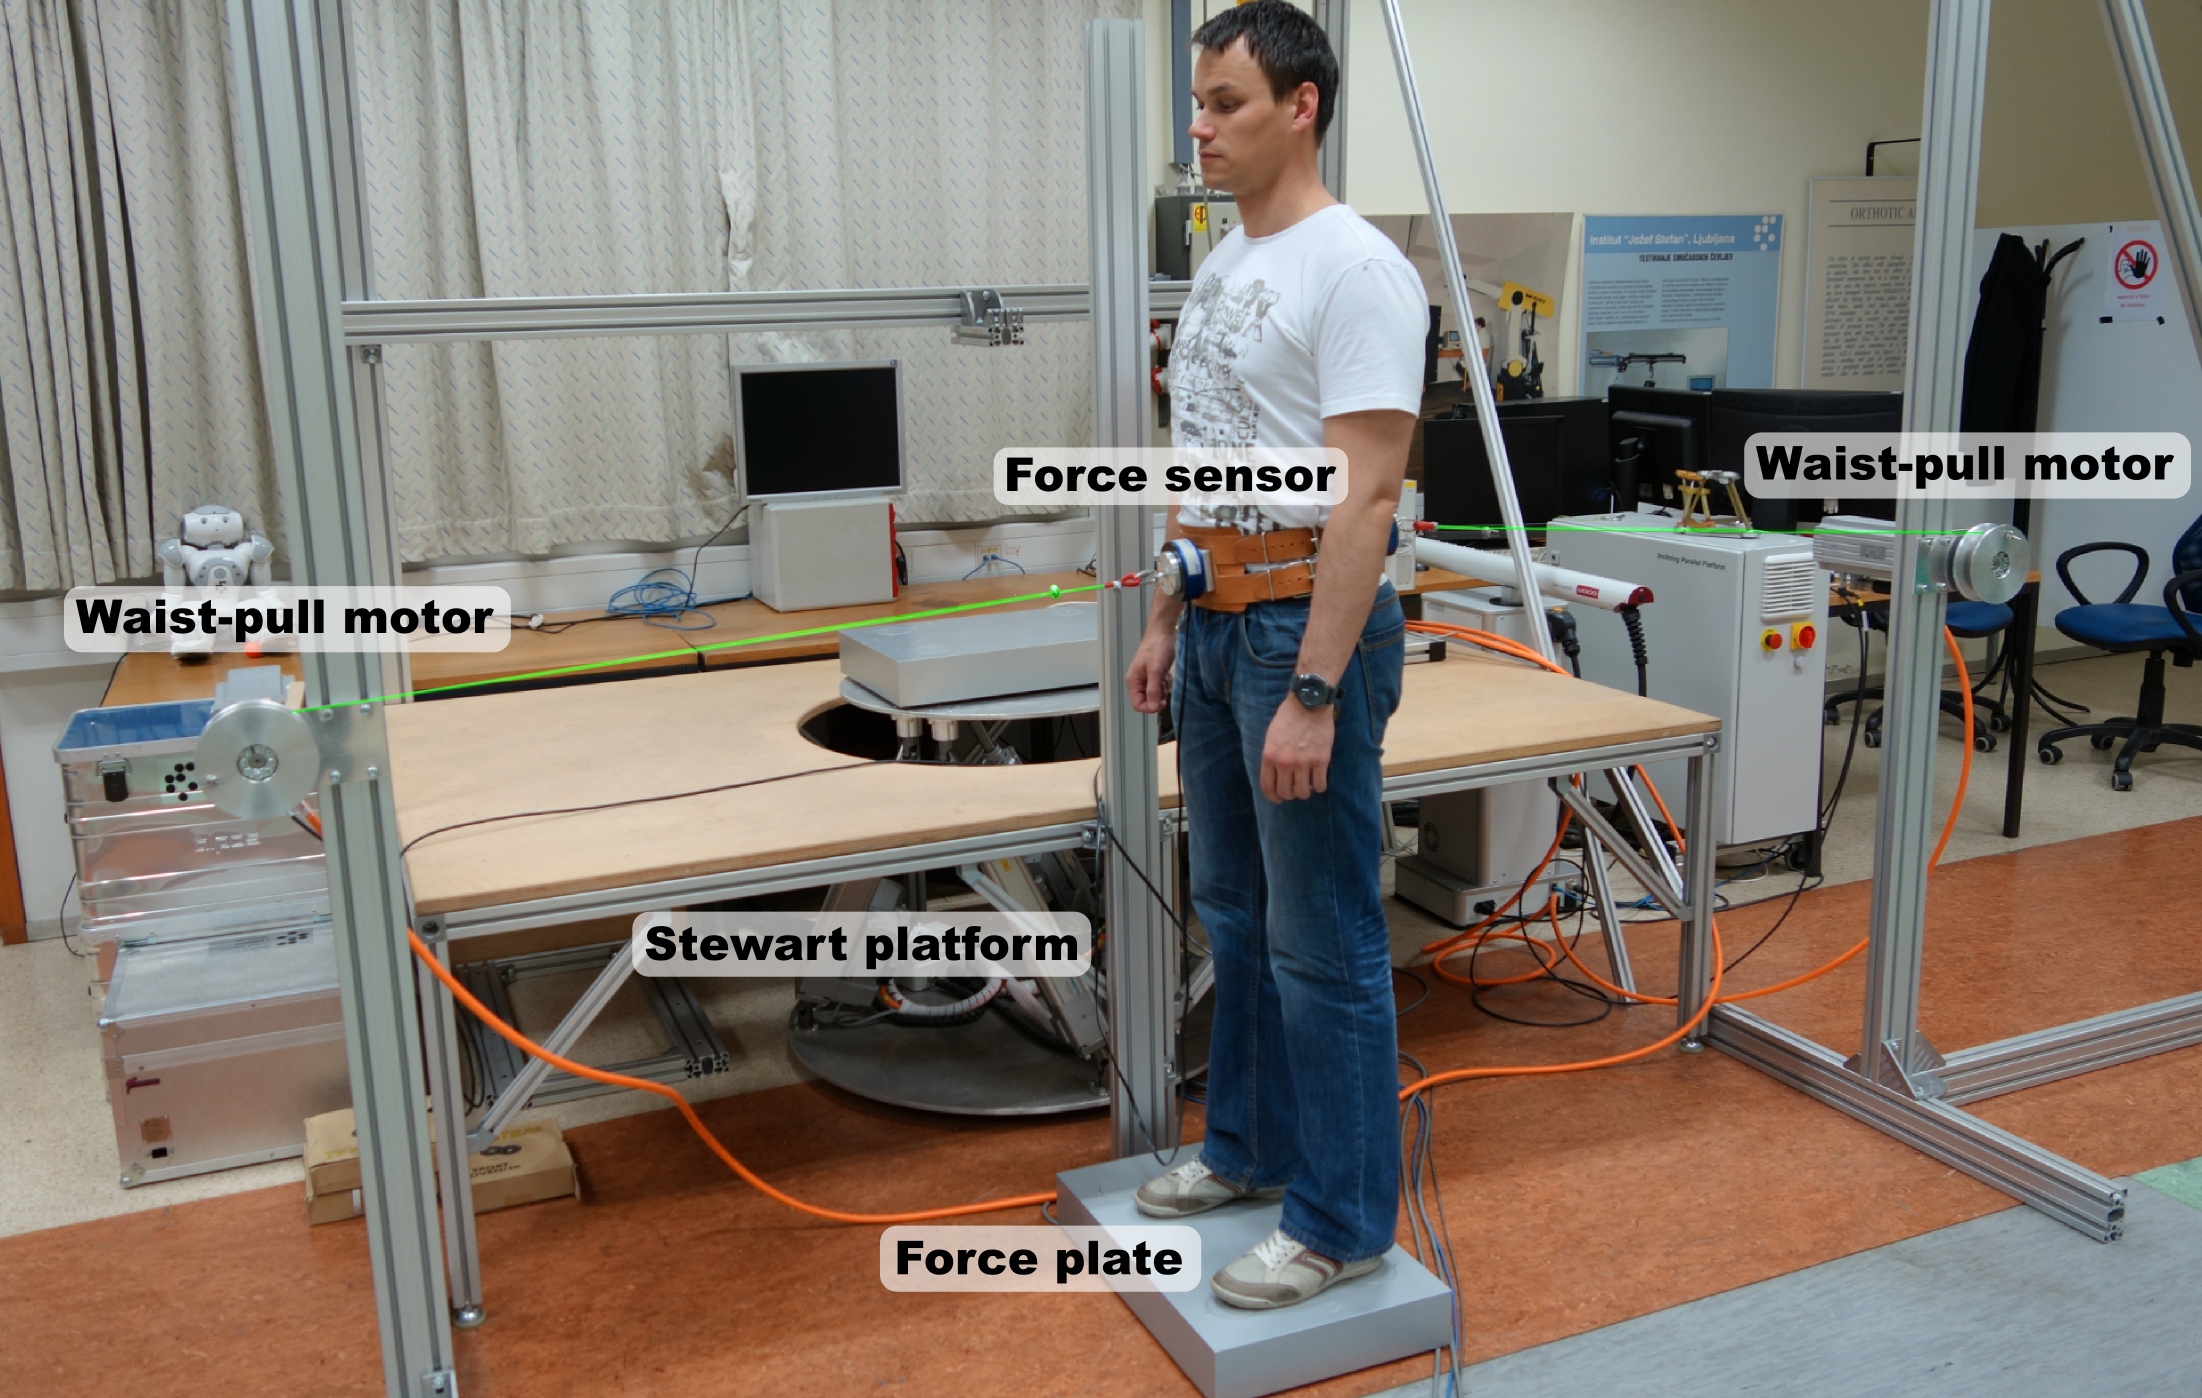
\includegraphics[width=0.8\hsize]{images/exp_setup_WP2.png}
%\caption{Experimental setup to study human postural control and whole body motion in contact with environment. Front and back waist-pull motors together with the two force sensors located at the subject's waist allow real-time force perturbations of the subject while the Stewart platform can perturb the balance by either translational or rotational motion (or a combination of both) of the support surface. Force plates are used in combination with kinematical and electromiographical measurements (not on the figure) to study the adaptation of subjects to the given perturbations.}
%\label{fig:exp_protocol_W2}
%\end{figure}

%\subsubsection{Design of models for human whole body motion in contact}
\subsection{Design of models for human whole body motion in contact}
Some work has been performed on understanding how to derive simplified models of whole-body balance that will encapsulate the task relevant parameters of posture control with multiple contacts. 

\begin{figure}
\centering
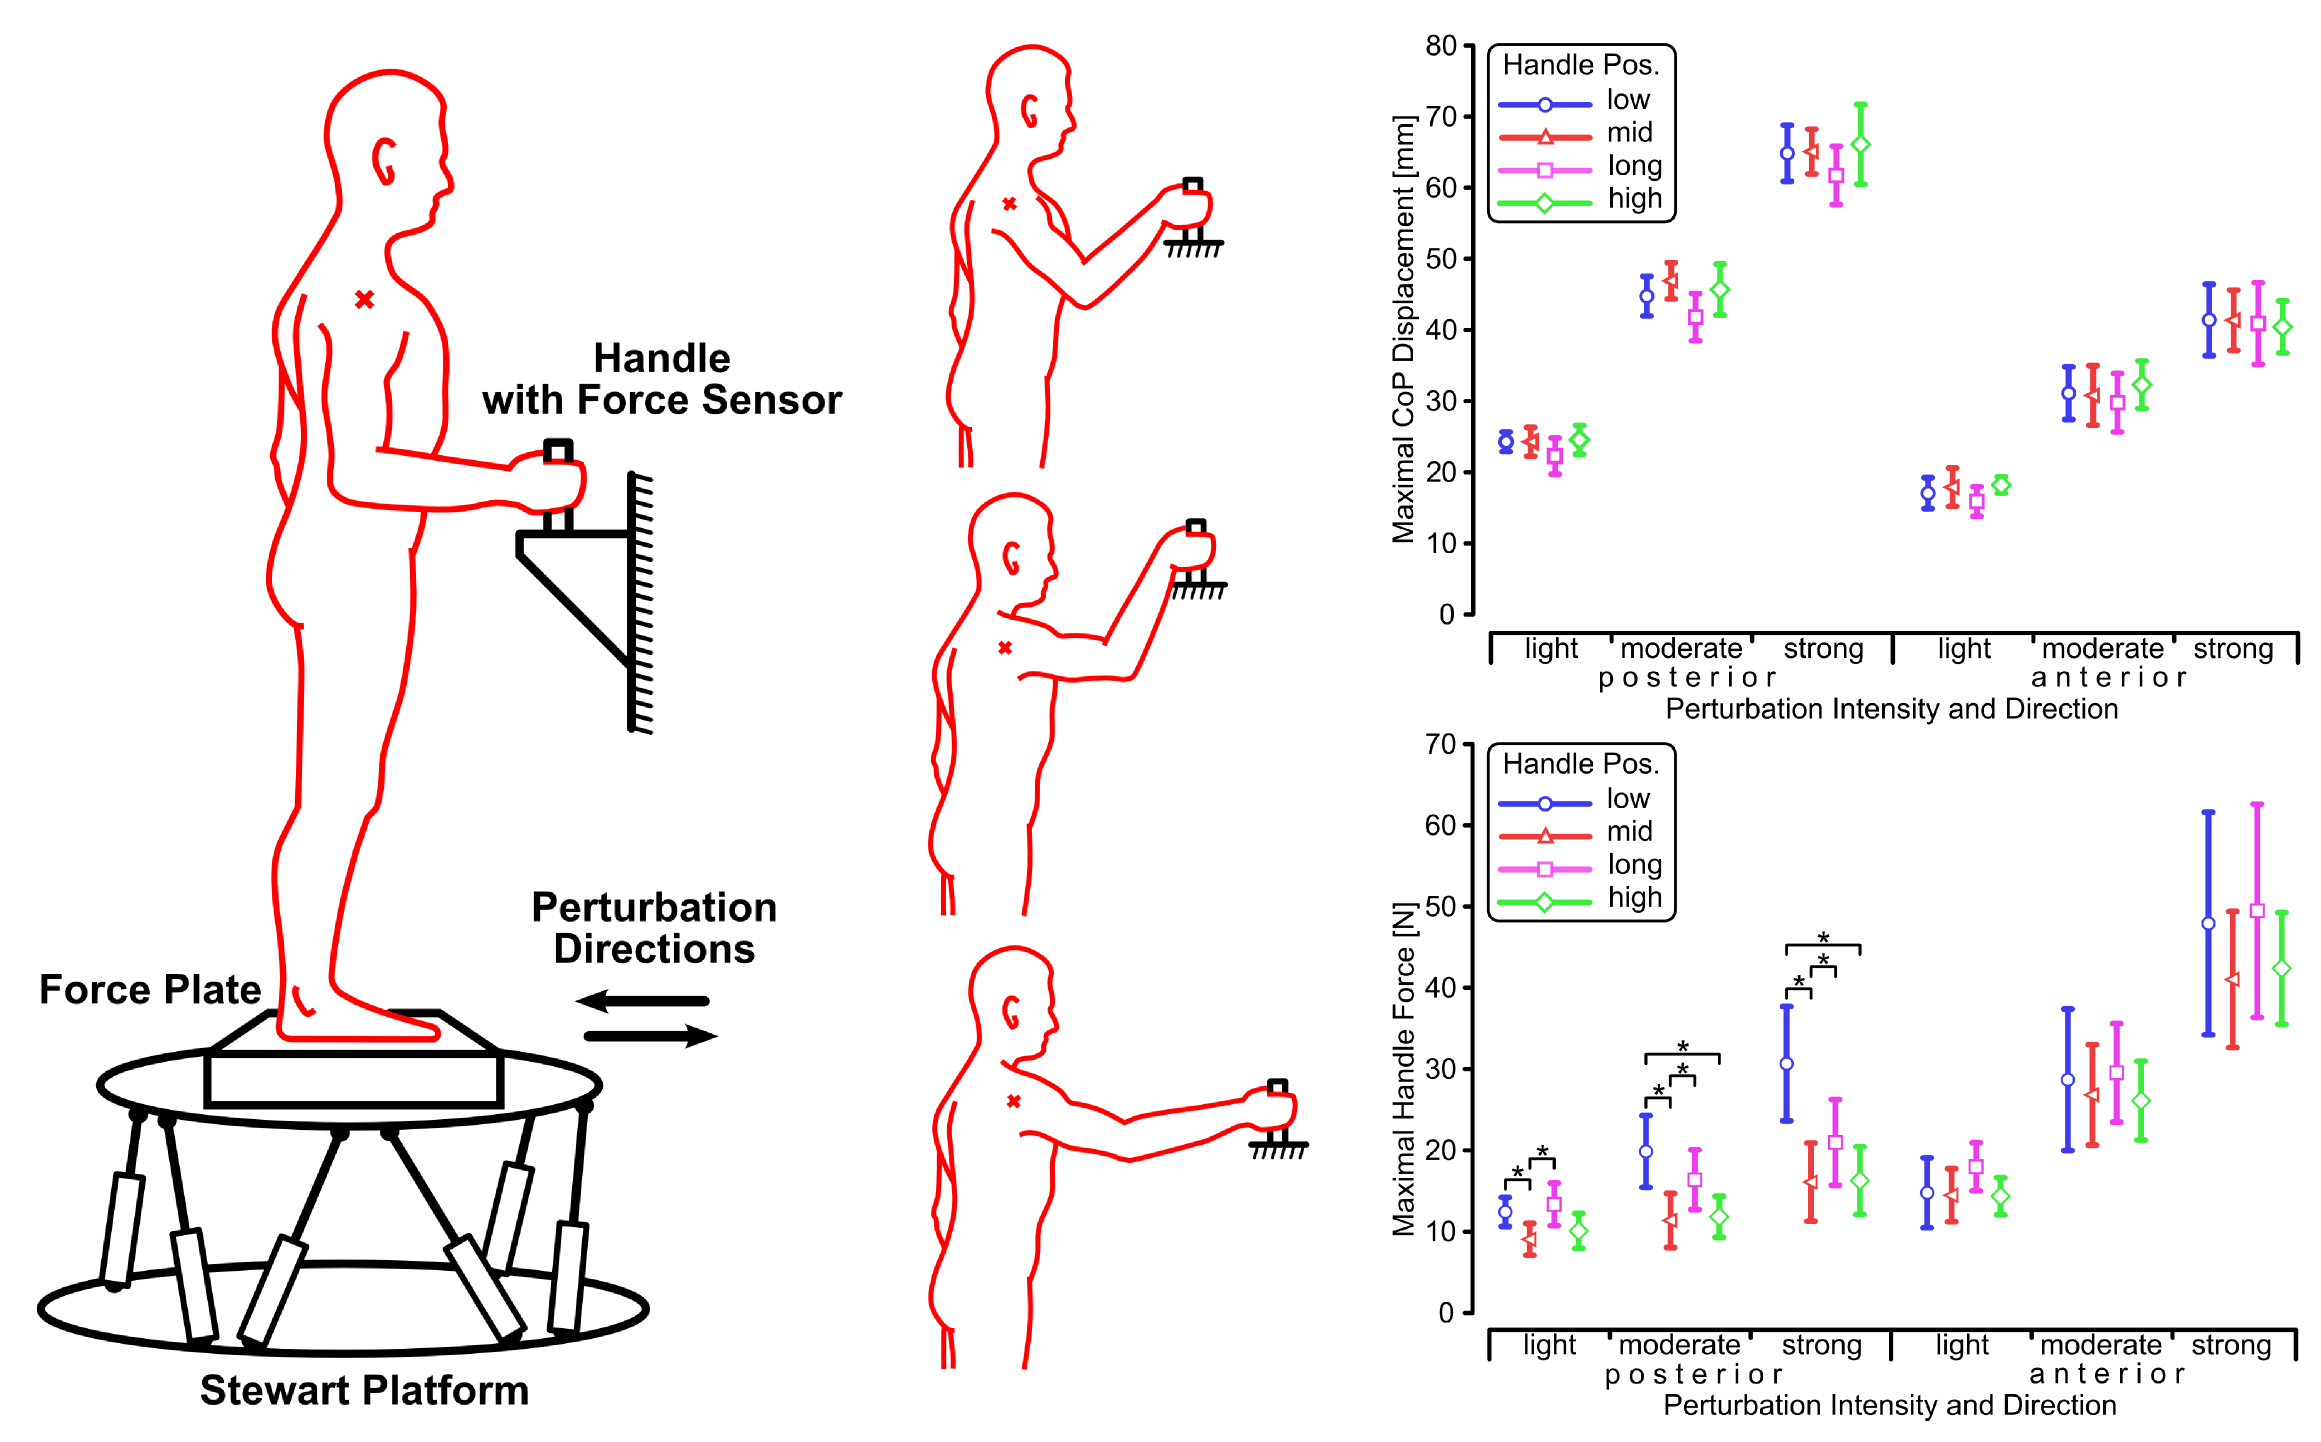
\includegraphics[width=\linewidth]{images/exp1_JSI.png}
\caption{Examining the functional role of a supportive hand contact. The subjects were standing on a force plate mounted on top of the Stewart platform that generated translational perturbations. The subjects were holding the handle with a built-in force sensor in four different positions. Major results of the study are shown on the two diagrams on the right side. Adapted from \cite{babivc2014effects}.}
\label{fig:exp_paper_W2}
\end{figure}

%\paragraph{Postural stability with multiple contacts}
\subsubsection{Postural stability with multiple contacts}
By emulating situations when balance of an individual is challenged, we examined functional role of supportive hand contact at different locations where balance of an individual was perturbed by translational perturbations of the support surface. The experimental methods are depicted on the left side of Figure~\ref{fig:exp_paper_W2}. We found that an additional supportive hand contact significantly reduced the maximal displacement of the subject's centre of pressure (CoP) regardless of the position of the handle and the type of the perturbation. On the other hand, the position of the handle had no effects on the maximal CoP displacement (top right diagram on Figure~\ref{fig:exp_paper_W2}) which is against the previous belief that the quality of postural control depend on the location of the hand contact \cite{Sarraf2014} and supports the idea that maintaining postural stability is the task of the highest priority and that the central nervous system does whatever necessary to keep the body balanced \cite{Winter1995}. Specifically, subjects always generated the required hand force, no matter where the location of the handle was, to keep the body balanced to the same extent. To get a better understanding of the functional role of supportive hand contacts, we examined the handle forces exerted by the subjects during the perturbation. In contrast with the effects on CoP, we found significant effects of perturbation direction, perturbation intensity and handle position on the maximal force in the handle (bottom right diagram on Figure~\ref{fig:exp_paper_W2}). A detailed description of these results can be found in  \cite{babivc2014effects}. A 3D dynamic model of a human holding to a stable object during continuous perturbations of stance was also created using OpenSim \cite{OpenSim}. The model was devised from measurements on 13 male subjects. Using the kinematical data recorded with frequency of 100Hz, forces that the subjects exerted on the ground, and the forces in the handle, we performed an inverse dynamic procedure and obtained joint torques produced by muscles during the experiment. An illustration of the model is shown in the left panel in Figure~\ref{fig:skeleton_ellipses}. Using this modelling approach we are now able to efficiently study the biomechanics of humans in contact with the environment.

%A study of  the effects of hand contact on the stability of a planar humanoid robot (see Figure~\ref{planarhumanoid}) while a momentum based controller is used to control the robot's balancing motion was  aslo performed \cite{Azad2014}. It compared the simulation results with the results of the experiments on human subjects which are reported in \cite{babivc2014effects}. Both simulations and experiments agreed that different values of hand contact forces in different hand positions cause the same displacements of the CoP of the foot. This implies that regulating the CoP of the foot has the highest priority for both humans and the momentum based  controller.  This study suggested that the momentum based controller is an adequate controller to replicate human behaviour during balancing motions.

\begin{figure}
	\begin{center}
		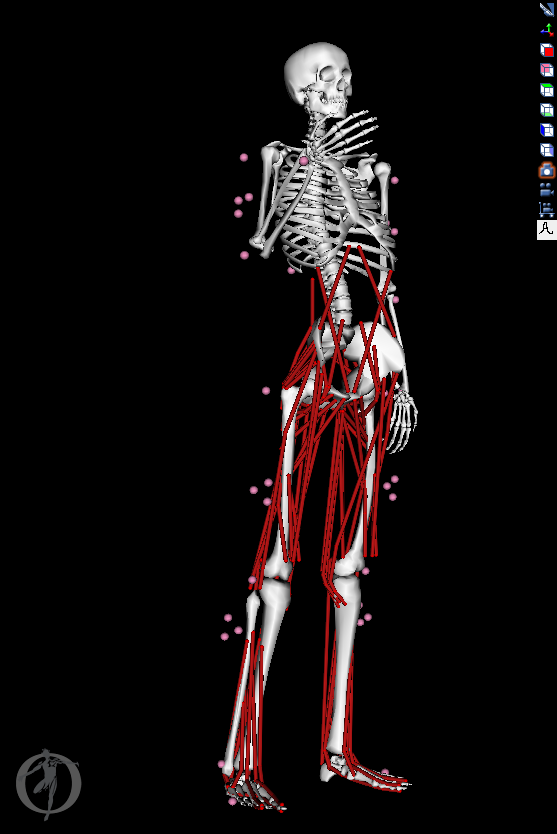
\includegraphics[height=5cm]{images/skeleton_v1.png}
		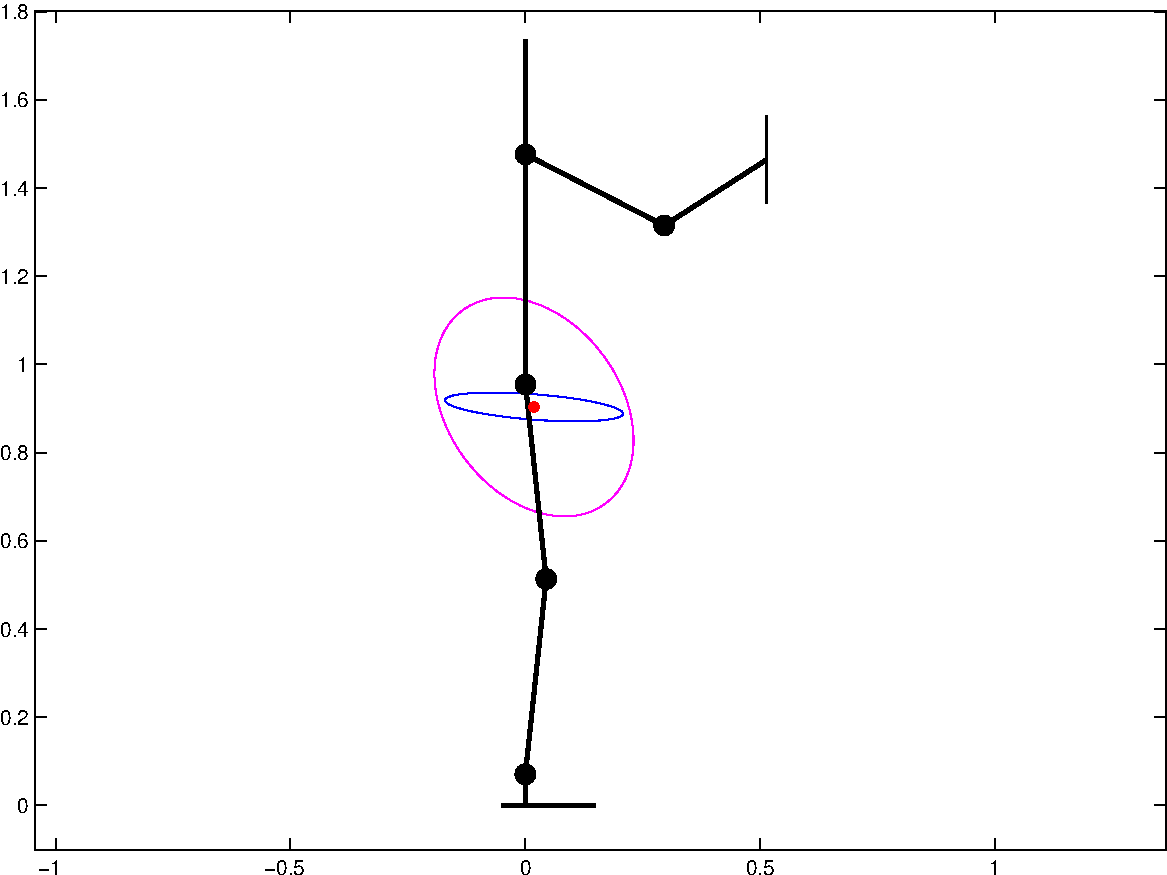
\includegraphics[height=5cm]{images/ellipses.pdf}
		\caption{Left: three dimensional model of a human subject holding a handle. Right: center of mass velocity ellipses for a planar humanoid robot.}
		\label{fig:skeleton_ellipses}
	\end{center}
\end{figure}

%\paragraph{Metric for postural stability with multiple contacts}
\subsubsection{Metric for postural stability with multiple contacts}
 A work on defining a suitable metric to measure the effects of the environmental contacts on the robot's stability was also undertaken.
It used the basic concept of end-effector manipulability (for manipulators)
in the literature and introduced a new tool to analyse the ability of balance
for legged robots which we called manipulability of the center of mass.
This tool relates the actuated joint velocities (all of them, \textit{e.g.} the ankle, the knee, the hip, the shoulder and the elbow ones for the planar humanoid robot described on the right side in Figure~\ref{fig:skeleton_ellipses}) to the linear velocity of the center of mass. It defines three different types of ellipsoids which are called 1)
velocity ellipsoid, 2) instantaneous velocity ellipsoid and 3) instantaneous
velocity ellipsoid due to the unit impulse.  The first one shows the velocity
of the CoM in different directions due to the unit norm of the joint
velocities.  The second and third types of the ellipsoids, which are obtained
by using impulsive dynamics, show instantaneous changes of the CoM velocity
due to the unit norm of instantaneous changes at the joint velocities and the
unit norm of impulse at the actuated joints, respectively.  By involving the
motion equations into the calculations for the second and third types of
ellipsoids (via impulsive dynamics), these ellipsoids allow us to study the
effect of under-actuation as well as kinematic constraints on the robot's
stability.

As an example, right panel in Figure~\ref{fig:skeleton_ellipses} shows a planar humanoid robot (with its hand is fixed) and instantaneous velocity ellipses for the robot in the specified configuration. Since the robot is fully actuated, the first and
second types of ellipses (type 2 and type 3) are the same. This ellipse (type
2) shows how the velocity of the CoM changes when the instantaneous change of
the joint velocities due to the impulse has the unit norm. This shows the
ability to move the CoM in different directions by a certain amount of
movements at the actuated joints. The ellipse type 3 shows how the velocity
of the CoM changes due to the unit impulse at the joints. In other words, it
shows how a certain amount of impulse at the actuated joints can accelerate
the CoM in different directions. All of the ellipses are independent from the
controller and they are dependent only on the physical parameters of the robot
and its kinematic constraints.

In balancing in a plane, the CoM movement in the horizontal direction is an
important measure. By projecting a velocity ellipse on $x$-axis, we obtain a
line which its length equals to the maximum change of velocity of the CoM in
the horizontal direction. Figure~\ref{type2} (left side) shows maximum
instantaneous change of the CoM velocity in the horizontal direction for
different constrained hand locations (\textit{i.e.} different elbow and shoulder
angles). This is due to the unit norm of instantaneous change of the joint
velocities. In the right side of this figure, the graph at the left side is
compared with the case that the hand is not constrained. It is obvious that
the movement of the CoM is limited due to the kinematic constraint at the
hand.
\begin{figure}[!t]
  \centering
  \begin{tabular}{lr}
    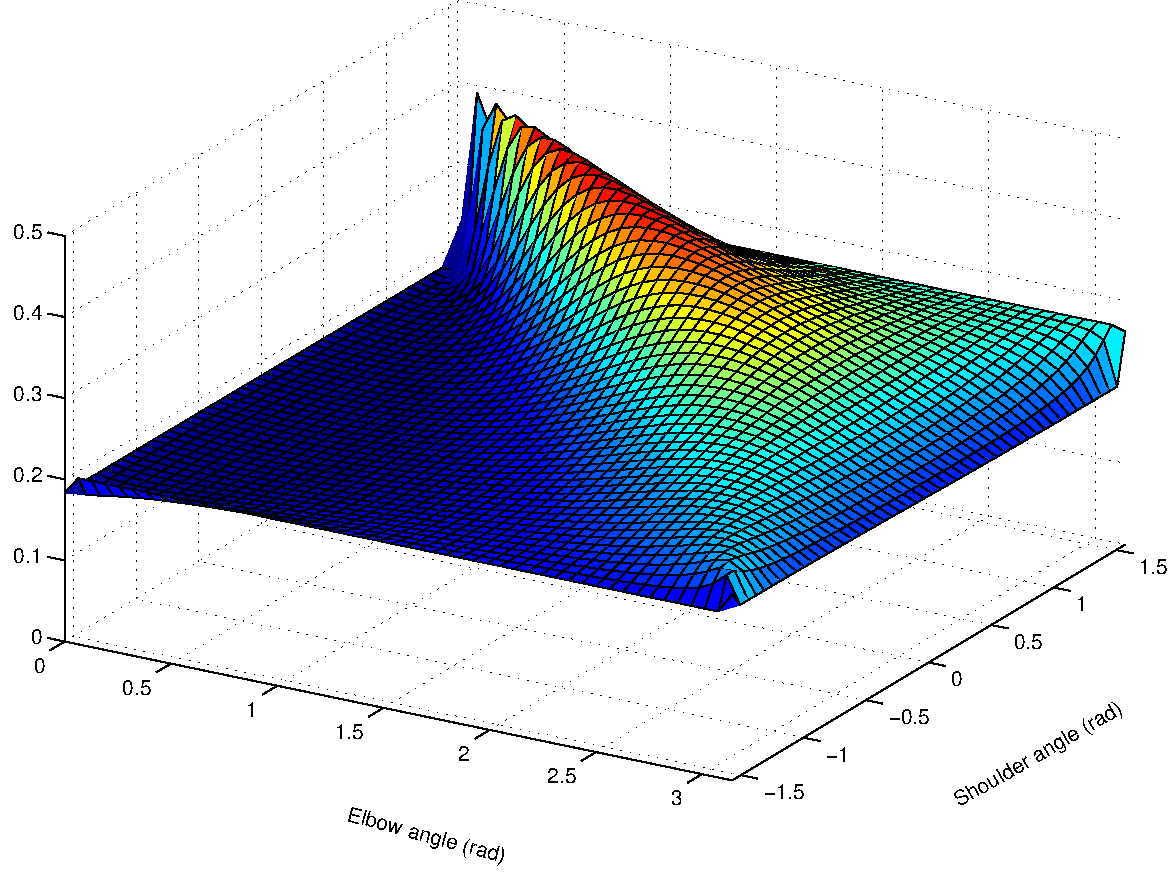
\includegraphics[width=0.5\linewidth]{images/type2_2.pdf}
    &  
    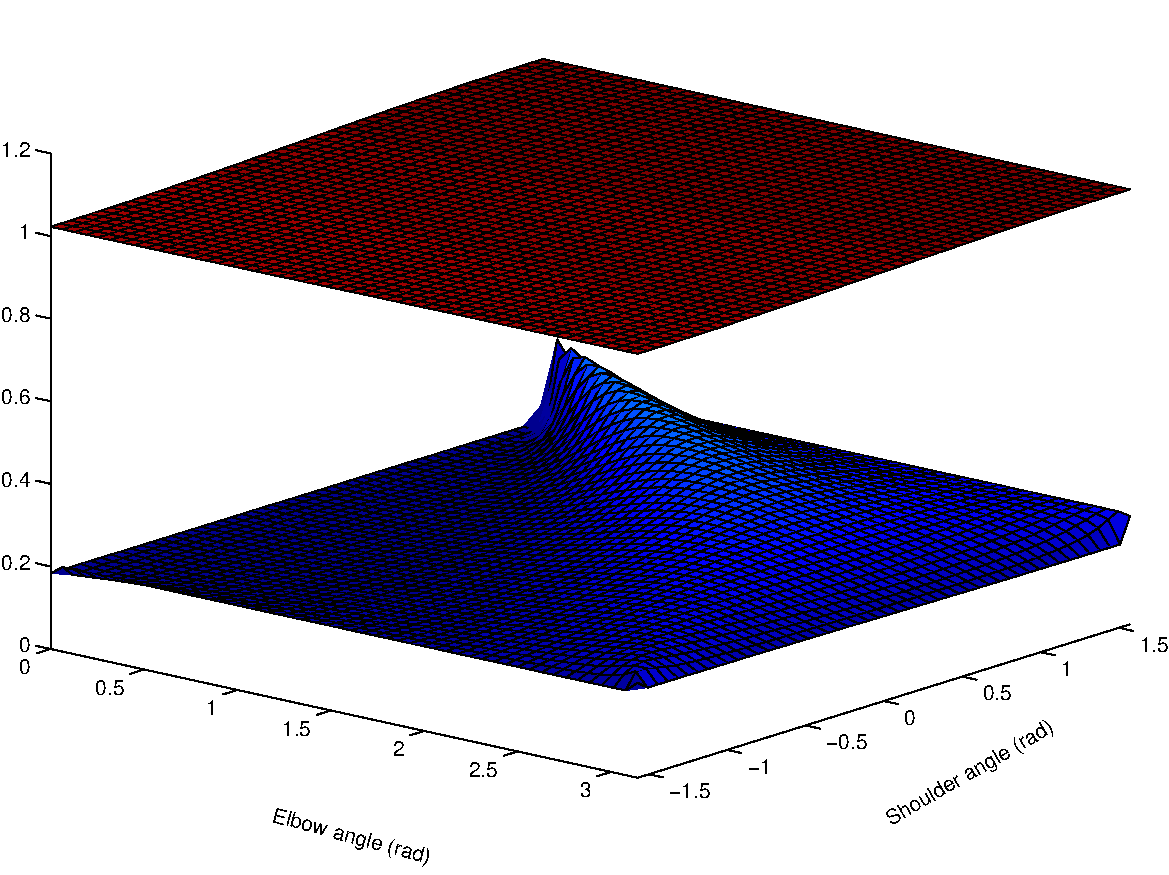
\includegraphics[width=0.5\linewidth]{images/type2.pdf}
  \end{tabular}
  \caption{Maximum instantaneous change of the CoM velocity in the $x$
    direction due to the unit norm of instantaneous change of the joint
    velocities for (left) the constrained robot and (right) for both
    constrained and unconstrained robots.}
  \label{type2}
\end{figure}

Figure~\ref{type3} shows maximum instantaneous change of the CoM velocity due
to the unit impulse at the joints for different hand locations and for both
constrained and unconstrained hands. As it can be seen in this figure, the
graph for the constrained robot is always higher than the other one. This
implies that the same amount of impulse can cause bigger changes at the CoM
velocity in the constrained robot rather than the unconstrained one. The
reason is that, in the constrained case, the robot exploits the contact force
to accelerate the CoM and therefore less (impulse) torque is needed for the
same change at the CoM velocity.
\begin{figure}[!t]
  \centering
  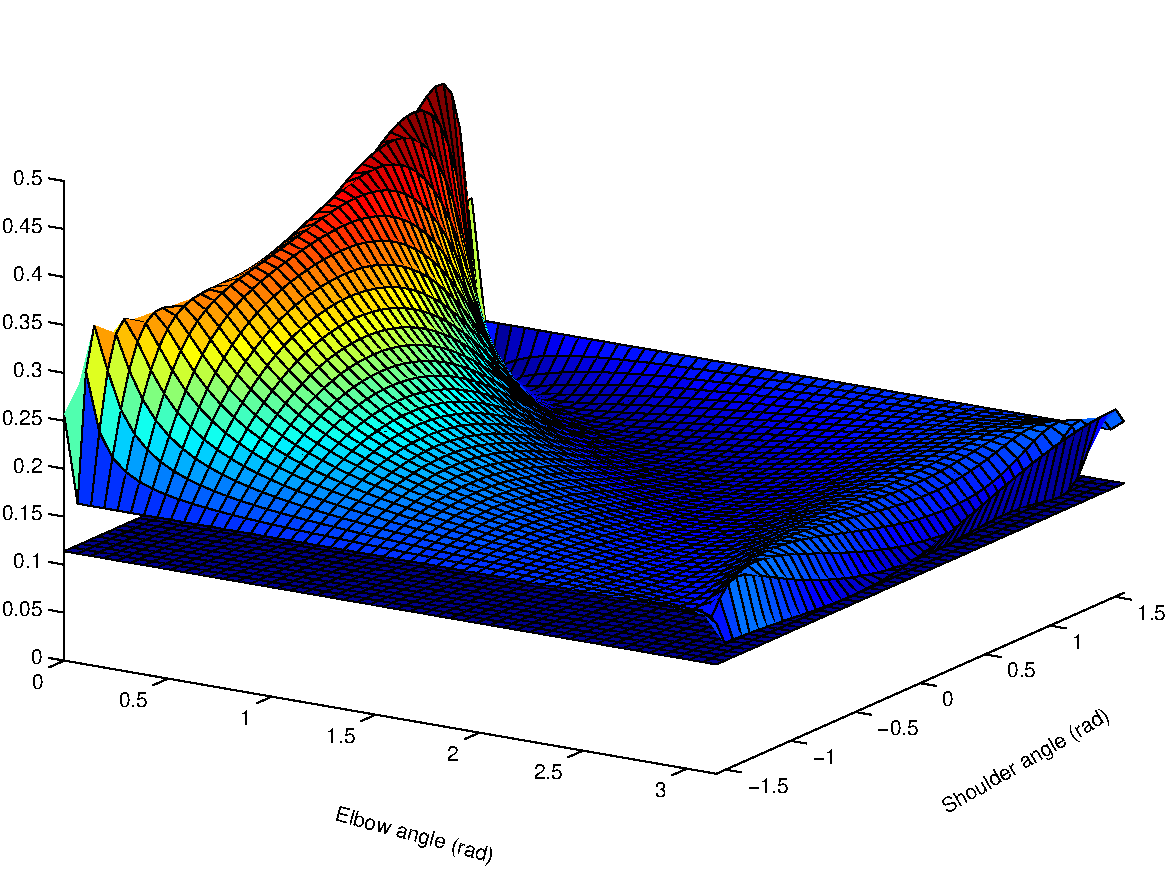
\includegraphics[width=\linewidth]{images/type3.pdf}
  \caption{Maximum instantaneous change of the CoM velocity in $x$ direction
    for the constrained and unconstrained robots due to the unit norm of
    impulse at the joints.}
  \label{type3}
\end{figure}




%\subsubsection{Strategies of dealing with uncertainties in contact}
\subsection{Strategies of dealing with uncertainties in contact}
A novel method to study human strategies of dealing with contacts with uncertain environment was developed. In this method a human subject was made to perform psychical
 contacts with the environment through the robot. The human was included into the robot control loop through human-robot interfaces. The idea is that the human sensorimotor system and cognitive system controls a novel mechanical system, \textit{i.e.} the robot, in physical interaction with the environment. This implies additional human motor control learning and adaptation that can potentially provide us with a deeper insight into how humans deal with a novel environment.

Another advantage of this approach is that the human sensorimotor system does not use its own limbs to directly make the contacts with the environment, but uses the robotic limb to do so. Compared to pure biomechanical studies, where the measured human behaviour must be further interpreted, adjusted or transformed before it can be used on the robots, in this approach the measured human behaviour can be directly captured and used in the robot control. This study therefore provides a good complement to our conventional biomechanical studies.

The block scheme of the proposed approach is shown in Figure~\ref{fig:scheme}. The human controlled the motion of the robotic limb with the motion of his/her own limb. In addition to controlling the motion, the human also controlled the impedance of the robot. Primary information about the robot state was relayed to the human through a visual feedback. A haptic device was used to provide the human with an additional feedback about the forces sensed by the robot. While controlling the robot in the proposed human-in-the-loop approach, the human central nervous system had to adapt to a new mechanism through sensorimotor learning to perform the desired contact with the environment.
\begin{figure}[!t]
  \centering
  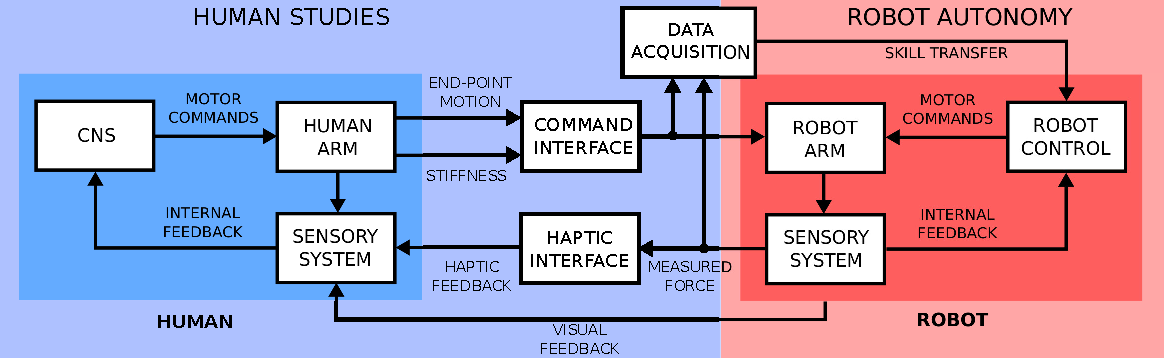
\includegraphics[width=\linewidth]{images/scheme.pdf}
  \caption{Block diagram of proposed human-in-the-loop robot control framework for study of human behaviour in contacts with environment. During the learning and adaptation stage, the human performs the contacts with the environment through the robot (blue section). The acquired data was used to observe and study the human behaviour. When the human learning process and observation is complete, the learnt skill can be directly captured and used in the autonomous robot control (red section). This is the main advantage compared to the conventional biomechanical studies.}
  \label{fig:scheme}
\end{figure}

The main goal of studies of human behaviour in contacts with environment is to offer a basis from which we can devise equivalent humanoid robot behaviour. The most appealing prospect of the proposed approach to study human motion in contacts with the environment is that the data from the study can be used to directly form skills for autonomous robot control. The sensorimotor data was collected while the human was making the desired physical contacts with the environment though robotic mechanism. This data was then used to form the trajectories. The trajectories were encoded with Dynamical Movement Primitives (DMPs) \cite{Ijspeert2002}. The parameters of DMPs were learned by locally weighted regression \cite{Schaal1998}. The learned trajectories represented the robot skill for dealing with the contacts with the environment according to the human strategy. The trajectories can be included into the robot control system and used for autonomous execution of the learnt task.
\begin{figure}[!t]
\centering
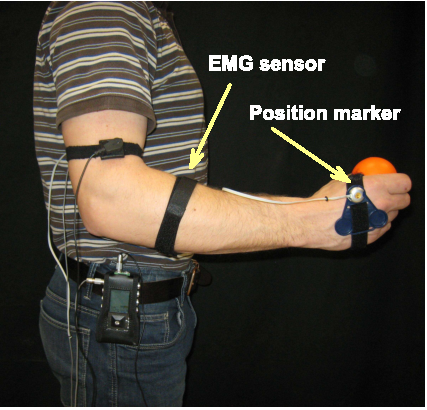
\includegraphics[height=3cm]{images/emg_setup.pdf}
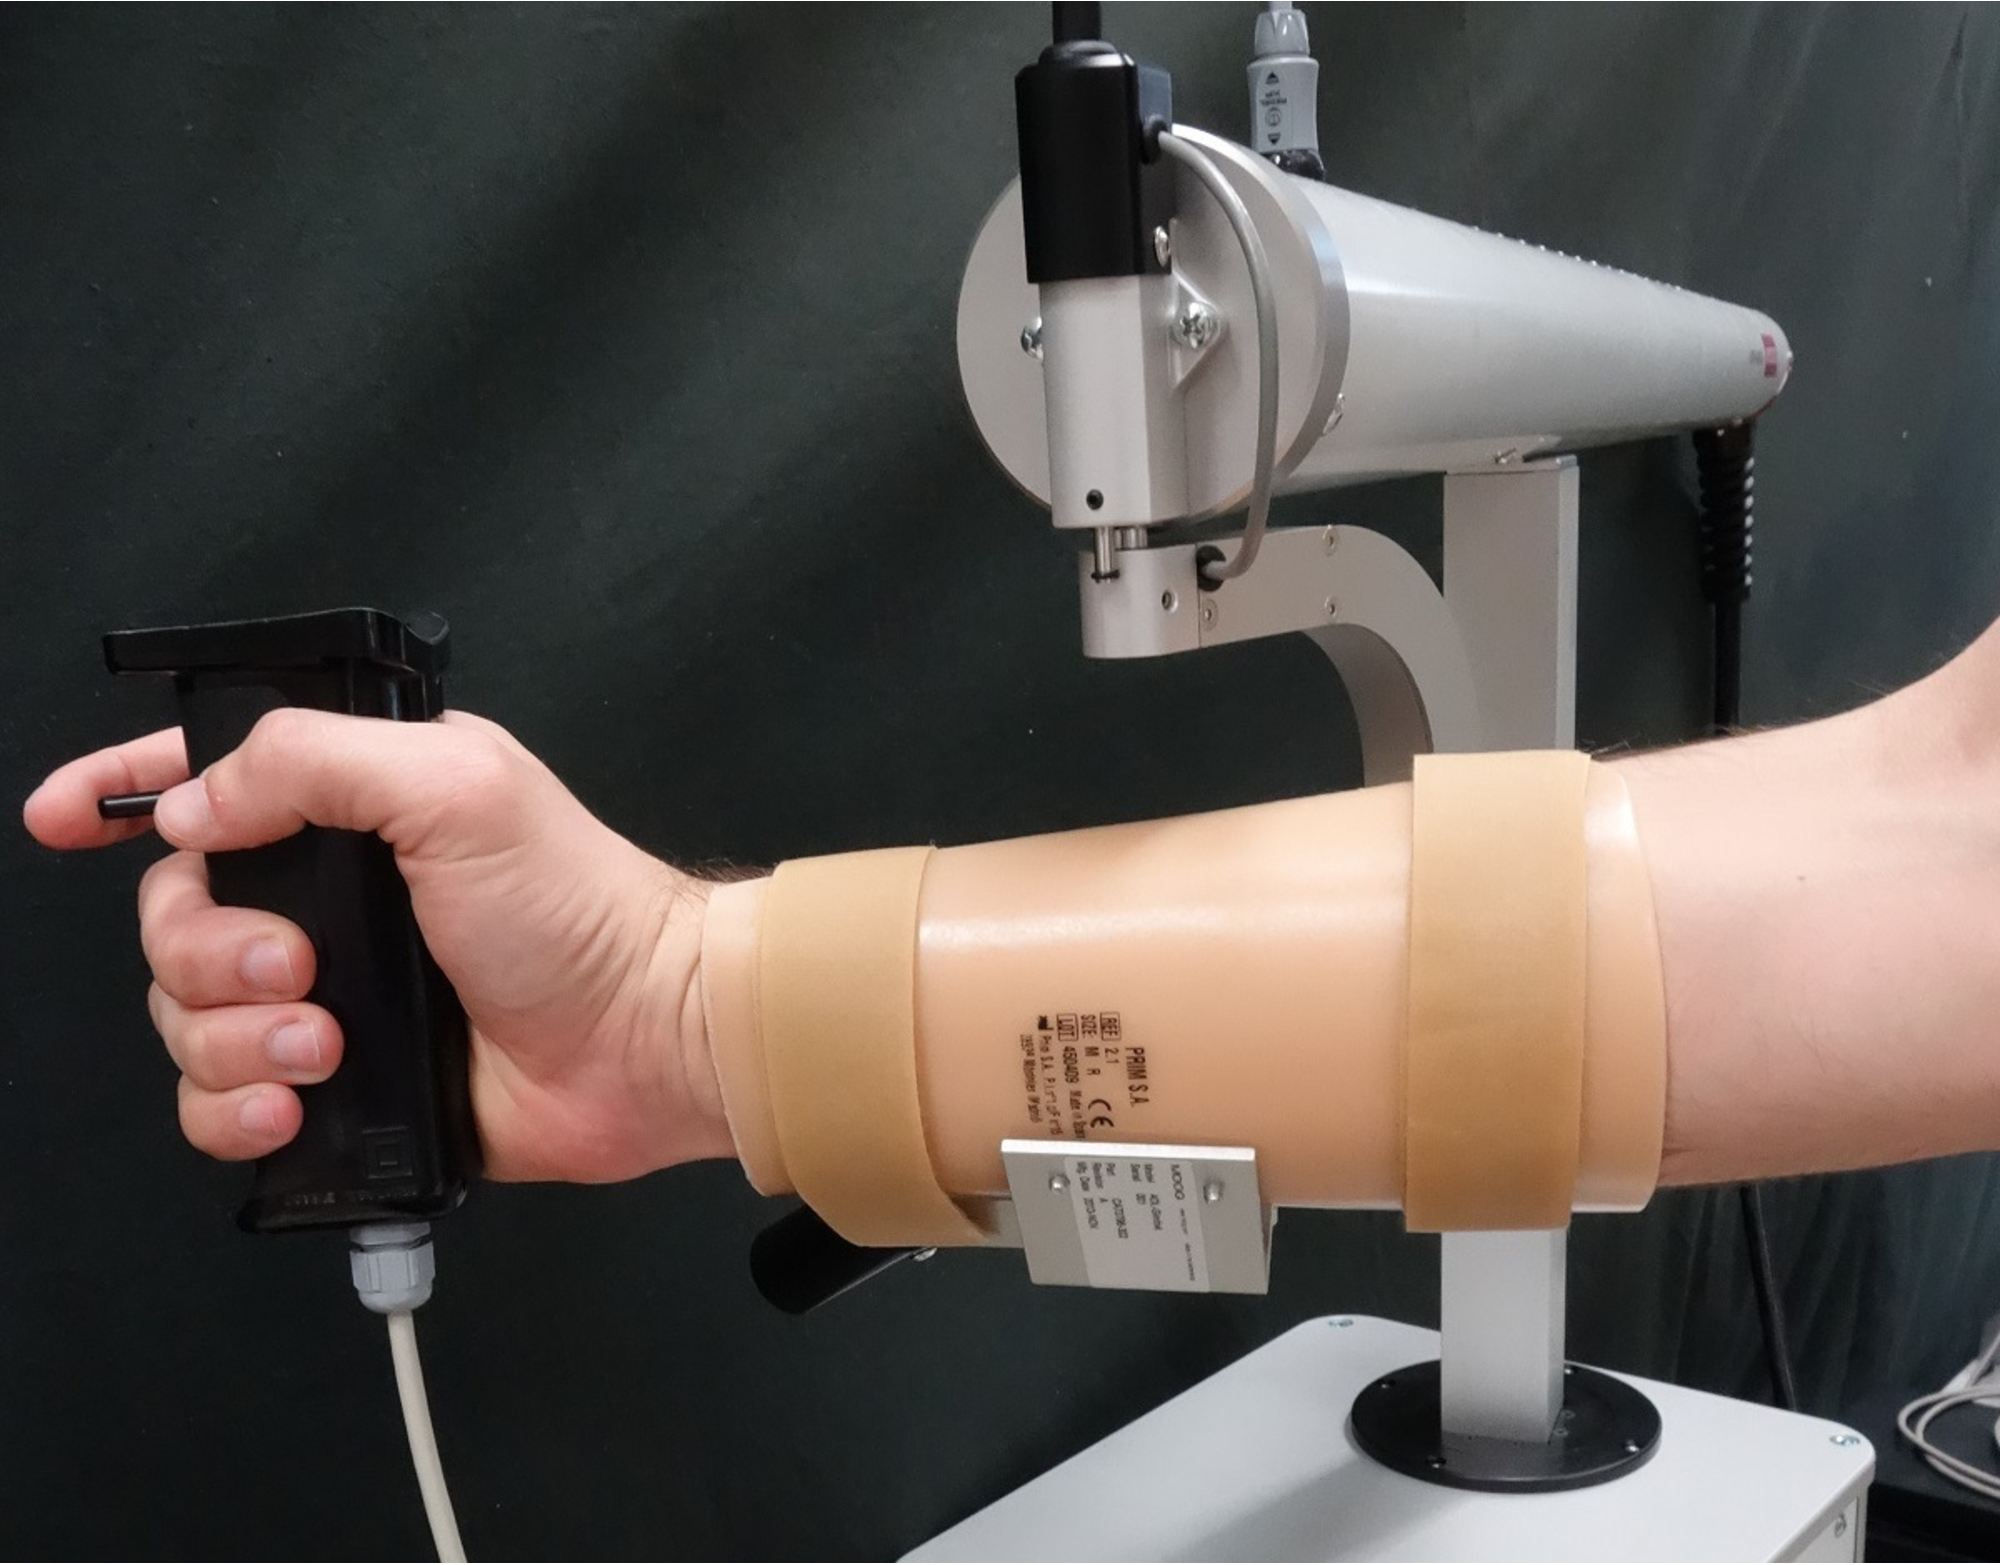
\includegraphics[height=3cm]{images/haptic.pdf}
\caption{Human-robot interfaces. First developed interface (left) measured human limb motion via optical motion capture system and mapped it to the motion of the robotic limb. The human muscle activity was measured by sEMG and was used as an interface to control the robot impedance. Second developed interface (right) consisted of \textit{HapticMaster} robot and impedance control handle. \textit{HapticMaster} robot measured the human limb position and provided the force feedback. Impedance control handle was based around a spring-return linear potentiometer and was held in the human hand.}
\label{fig:interface}
\end{figure}

One of the key features of the proposed approach is the ability of the human to directly control the impedance of the robot limb in an equivalent way that he/she controls his/her own. For this purpose we developed two novel human-robot interfaces \cite{Peternel2014,Peternel2015} that allow the human to modulate the stiffness of the robotic limb in real-time. The first interface (see Figure~\ref{fig:interface}, left) was based on measuring human muscle activity by surface electromiography (sEMG). The current measured muscle activity was mapped to the robot stiffness. The second interface (see Figure~\ref{fig:interface}, right) was based around a linear potentiometer inside a handle held in the human hand. The human controlled the position of the potentiometer knob with a finger position. The finger position is then mapped to the robot stiffness via measured potentiometer voltage.




%\subsubsection{Human contact choice and learning through physical interaction}
\subsection{Human contact choice and learning through physical interaction}
In order to understand how humans make contact choice decisions (\textit{e.g.} whether or not to initiate a hand contact, and where to place the hand), we need an estimation of joint torques as well as a metric of stability in various multi-contact situations.

%To understand the factors involved in human choice of contact utilization, we performed a series of experiments where the subjects were standing still with arms hanging freely at the sides. The parallel platform induced a randomly timed series of perturbations of different accelerations, velocities and displacements. The aim of the experiments was to investigate what profile of support perturbation forces the human to make a supportive hand contact with environment and how human chooses the location of the hand contact with regard to the direction of the perturbation. Interestingly, we found that the subjects reacted to every perturbation no matter how small or slow the perturbation was or what was the initial acceleration of the perturbation. The reactions were manifested as muscle twitches of shoulder or as unspecific arm motions that were unrelated to the proximity of possible support objects. The reactions occurred also at the smallest perturbations when no actual correction of balance was needed. Our experiments showed that these reactions are essentially protective reactions rather than reactions that have counterbalancing effects \cite{McIlroy1995, Corbeil2013}.


%These reactions mask the real factors involved in human choice of contact utilization. We therefore altered the perturbation methods for our further experiments and designed continuous random perturbations in a frequency band that corresponds with typical human motion during postural control \cite{Nawayseh2006}. By doing so we excluded the effect of surprise that evoked the reflex reactions of humans. This will hopefully allow us to uncover the factors involved in human choice of contact utilization.\\

\begin{figure}
	\begin{center}
		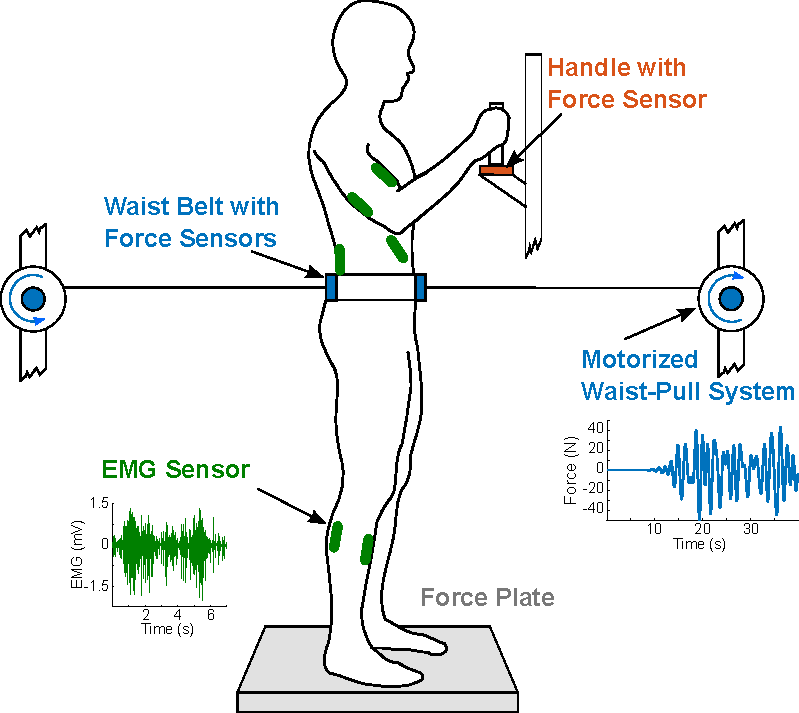
\includegraphics[width=\linewidth]{images/exp2_protocol.pdf}
		\caption{The subject was standing on a force plate, connected to the motorised waist-pull system that generated translational perturbations. The subject was holding the handle with a built-in force sensor mounted on a vertical pole. EMG electrodes were positioned on the major body muscles of the subject's right-hand side.}
		\label{fig:exp2_protocol}
	\end{center}
\end{figure}


%\paragraph{Motor adaptation with supportive hand contacts}
\subsubsection{Motor adaptation with supportive hand contacts}
In continuation of this work, we studied how additional hand contact with the surrounding objects influences whole-body balance conditions. The experiments were performed on multiple subjects where we challenged their balance. The experiments were divided into two main stages. Each stage had 15 sessions in which the subject's balance was perturbed for 5 minutes. In one stage the subjects did not use supportive hand contact. In the other stage they were holding a handle in front of them. We used a motorised wait-pull mechanism \cite{Peternel2013} to continuously perturb the balance of the standing subjects in either stage by exerting external forces on the approximate position of centre of mass. See Figure~\ref{fig:exp2_protocol} for the experimental setup. The perturbation waveform of the waist-pull mechanism was constructed in a way that the possible muscle reactions associated with reflexes were eliminated. These reactions could potentially mask the actual role of the hand muscles as the reflex would activate the muscles unrelated to the magnitude of the perturbation. To avoid that, the perturbation waveform was continuous, had relatively low frequency and low pulling forces. During the experiment, we measured muscle activation of the subject's lower leg, trunk and arm muscles, forces in the handle and the anteroposterior movement of CoP (CoP$_{AP}$). The results of muscle activation analysis showed that when the subjects were holding to the handle, the activation of the leg muscles was minimal (see Figure~\ref{fig:representativePSD}). Based on this we can conclude that the subjects mainly used their arm muscles to maintain postural stability. The trunk flexor muscle (Obliques Externus, OE) was more active in the stage when the subjects were holding the handle compared to when they were not. This indicates that a synergy between the arm and trunk muscles was established when additional hand contact was utilised to maintain the equilibrium.

\begin{figure}
	\begin{center}
		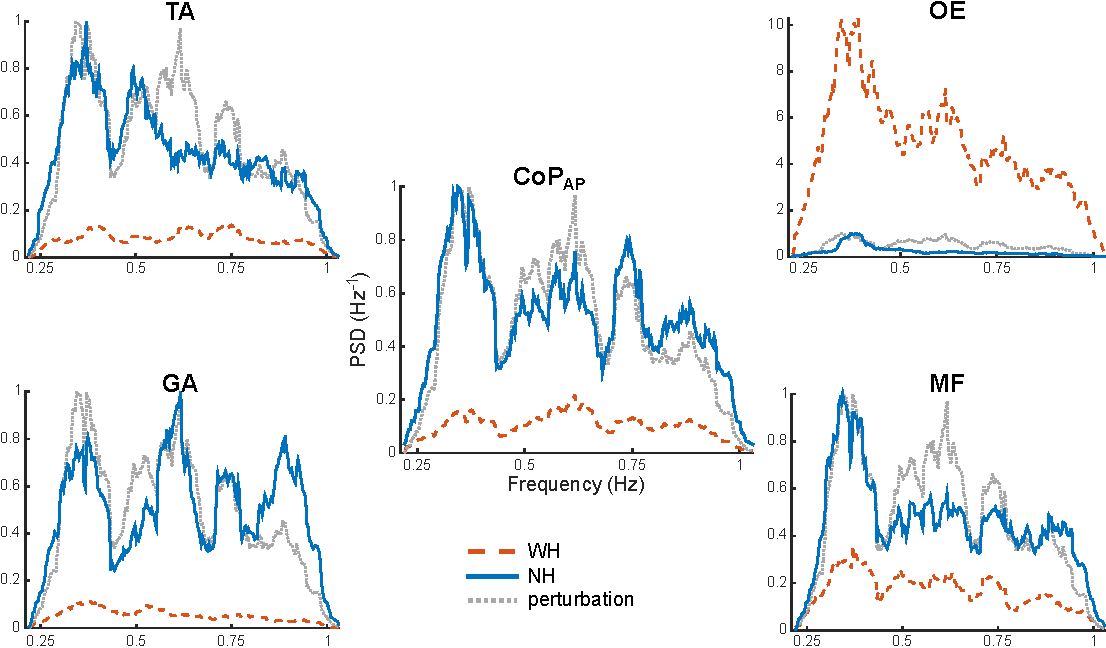
\includegraphics[width=\linewidth]{images/representativePSD_oneYaxis-v1.pdf}
		\caption{Effect of holding a handle after adaptation stabilised in the last session. The graphs show representative power spectral density (PSD) profiles of CoP$_{AP}$ and muscle activations measured in trunk and lower leg muscles. After the adaptation, effect of additional supportive hand contact stabilised to the perturbation in the last session. All EMG and CoP$_{AP}$ values are presented in a frequency domain, ranging from 0.25 Hz - 1 Hz. The blue (solid) lines represent the power in no-handle and the orange (dashed) lines in handle stage. The grey (dotted) line is the power of the perturbation signal. All signals are normalized to the peak value in the last session. The effect of handle is shown as reduced muscle activation in all muscles in the handle session, except in the trunk flexor muscle (OE), where there is an opposite effect.}
		\label{fig:representativePSD}
	\end{center}
\end{figure}

The analysis of the CoP$_{AP}$ movement showed that the displacement of the CoP$_{AP}$ was progressively dropping throughout the repeated sessions of the experiment (see Figure~\ref{fig:COPapAndTau}). This was true both in case when supportive hand contact was used and in case when no supportive hand contact was used. These results give a strong hint that a learning and adaptation mechanism was present through the sessions of the experiment, as the subject gradually improved the balance control.

\begin{figure}
	\begin{center}
		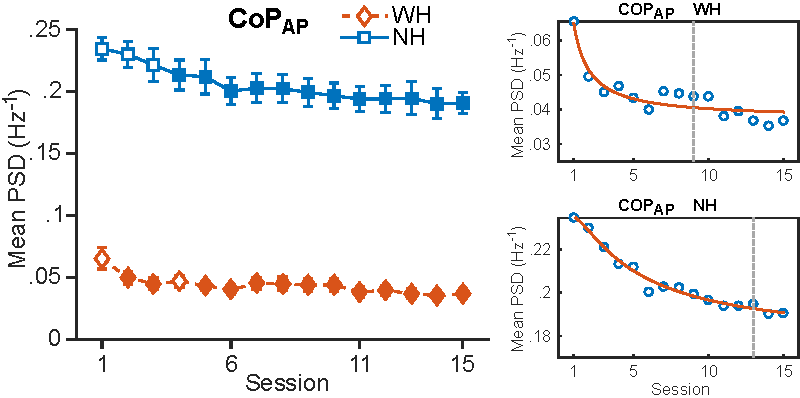
\includegraphics[width=\linewidth]{images/COPapAndTau.pdf}
		\caption{Adaptation of movement of CoP$_{AP}$ is shown on the left graph. Experimental stage with handle (WH) is shown in red, while condition without handle (NH) is shown in blue. Full markers indicate statistically significant differences between the first session and each of the following sessions. In both stages the adaptation is statistically confirmed ($p < 0.001$). In the stage where the subjects were holding the handle, the adaptation appeared right after the first session. In no-holding stage it appeared after the third session. The superimposed best-fit curves are shown on the right graphs with orange solid lines. A calculated session number at 3$\tau$ of the fitted curve (vertical dotted line) indicates faster stabilisation of adaptation in the handle stage, compared to no-handle stage.}
		\label{fig:COPapAndTau}
	\end{center}
\end{figure}


We further analysed whether there are any effects of repeated sessions on adaptation of muscle activation and movement of CoP$_{AP}$, and whether there are any differences between the two stages of the experiment. The results show that the effect of human adaptation in lower leg muscles was statistically significant in the stage when the subjects were not using the additional hand support. However, this was not the case for the stage when the subjects were holding to the handle. The activation of the trunk extensor muscle (MF) was almost the same in both stages and throughout all sessions. On the other hand, the activation of the trunk flexor OE remained unchanged throughout the sessions only in the stage when subjects held the handle. The activation of OE was much higher in this stage compared to stage when subject did not use supportive hand contact.

\begin{figure}
	\begin{center}
		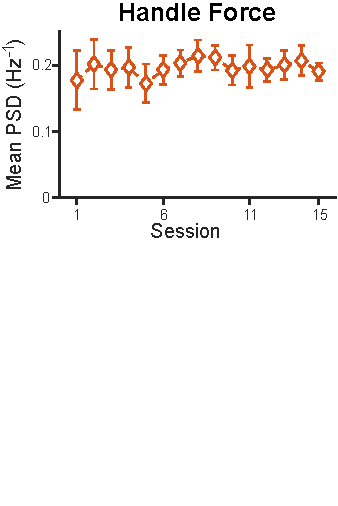
\includegraphics[width=0.7\linewidth]{images/HandleForce-all-1.pdf}
		\caption{Absence of effect of the repetition of sessions one the handle forces.}
		\label{fig:HandleForces}
	\end{center}
\end{figure}

We performed an analysis of differences in EMG activation levels between the two experimental stages in the frequency spectrum of the perturbation waveform (low = 0.25 - 0.5 Hz, medium = 0.5 - 0.75 Hz, high = 0.75 - 1.0 Hz). A paired samples analysis between the two stages for low, medium and high frequency range revealed that there was an influence of additional hand contact on both lower leg muscles. There were confirmed statistically significant differences between the two stages in all frequency ranges and for all sessions. For the MF muscle these differences were not significant in any of the frequency range nor session. However, there were significant differences between the two stages for the OE muscle. These differences occurred in the medium and high frequency range but only in the last session. When the subjects were holding to the handle, we recorded the forces exerted on the handle during the continuous postural perturbations. Statistical analysis of handle forces revealed that the repetition of sessions had no significant effects (see Figure~\ref{fig:HandleForces}). Even though the activation of arm extensor muscle changed (decreased) during sessions, there was no significant change in forces applied on the handle.\\


We performed an analysis of differences in EMG activation levels between the two experimental stages in the frequency spectrum of the perturbation waveform (low = 0.25 - 0.5 Hz, medium = 0.5 - 0.75 Hz, high = 0.75 - 1.0 Hz). A paired samples analysis between the two stage for low, medium and high frequency range revealed that there was an influence of additional hand contact on both lower leg muscles. There were confirmed statistically significant differences between the two stages in all frequency ranges and for all sessions. For the MF muscle these differences were not significant in any of the frequency range nor session. However, there were significant differences between the two stages for the OE muscle. These differences occurred in the medium and high frequency range but only in the last session. When the subjects were holding to the handle, we recorded the forces exerted on the handle during the continuous postural perturbations. Statistical analysis of handle forces revealed that the repetition of sessions had no significant effects. Even though the activation of arm extensor muscle changed (decreased) during sessions, there was no significant change in forces applied on the handle.\\


\begin{figure}
\centering
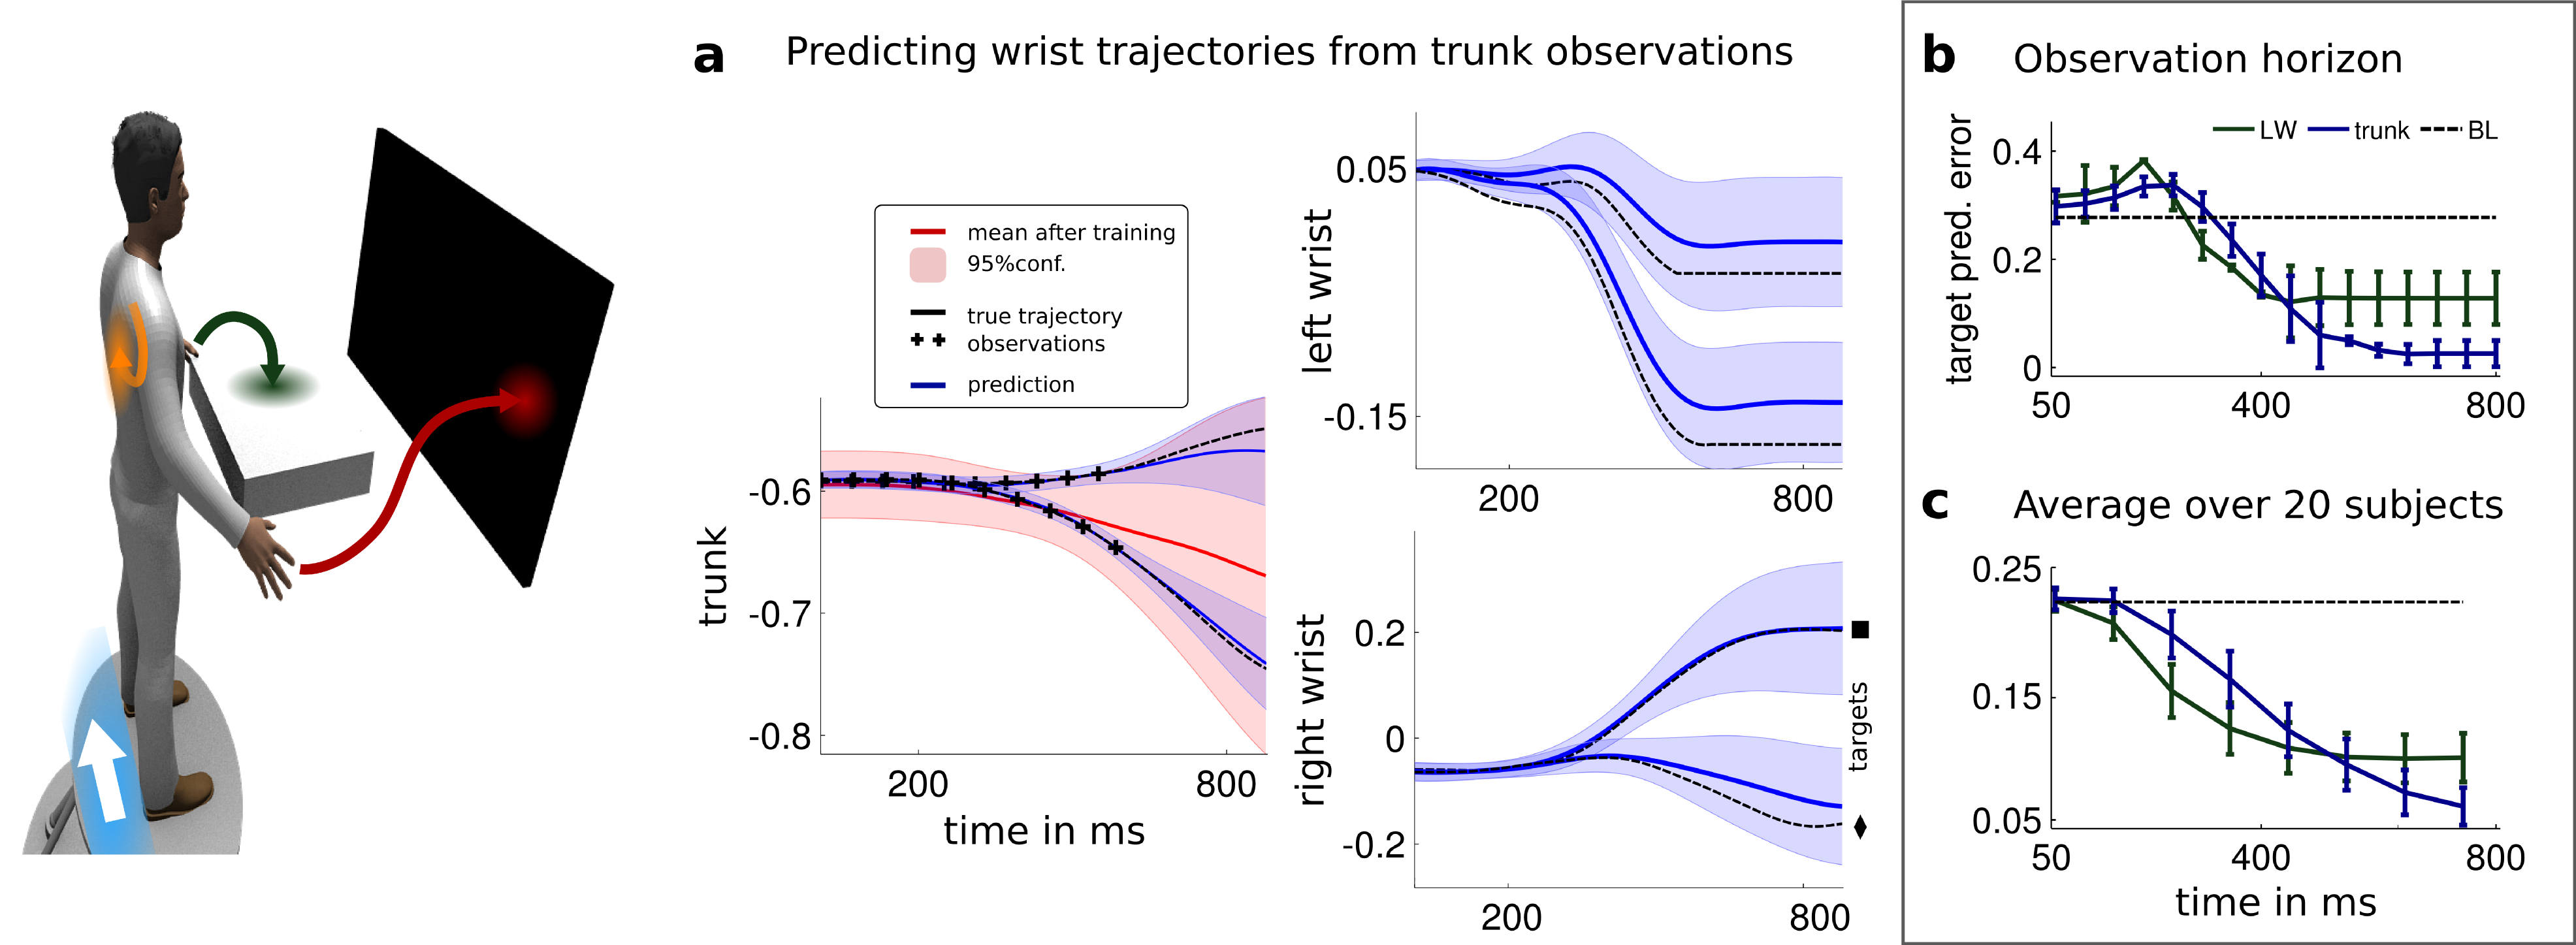
\includegraphics[width=\linewidth]{images/SummaryFig_Y2Report.png}
\caption{Trunk trajectories predict wrist trajectories. (a) 600ms of trunk trajectories are observed. These observations can predict the wrist trajectories. Shown are predictions for the two exterior targets on the screen. For training 10 trials for each target are used starting from trial 240 backwards in time (before the catch trials). For testing the first perturbed trial after trial number 240 were used. (b) The effect of the observation horizon on the target prediction error is shown for a representative subject. The mean of the training data denotes the base line (BL). (c) Average statistics (mean and 95 percent confidence bound) over 20 subjects.
}
\label{fig:HumanProMPsPrediction}
\end{figure}

%\paragraph{Planned \textit{vs} reactive contact models} 
\subsubsection{Planned \textit{vs} reactive contact models}
We studied whether supporting contacts in human arm reaching tasks are planned or an effect of a reactive controller. Investigations on human motor learning has focused on adaptation experiments with fixed contact points leaving research on the computational role of contacts as a free control variable unexplored. In perturbed target reaching experiments sketched in Figure~\ref{fig:HumanProMPsPrediction}, we studied weather supporting contacts are planned or reactive. Subjects had to reach for distant targets on a screen with their right hand. For reaching the target additional support through contacts with a table using the left hand was inevitably. If the contacts are planned then the left hand's motion can predict the right hand reaching. We studied how probabilistic inference in learnt models can be used to answer this question. Evidence for planned contacts could be provided through learning probabilistic models of trajectory distributions and using the models to generate predictions, Figure~\ref{fig:HumanProMPsPrediction} (a). We found that the target on the screen could be predicted from both, the left hand (mse: $10.4$cm $\pm$ $2$cm over $20$ subjects) and the trunk movement (mse: $6.7$cm $\pm$ $1.4$cm over $20$ subjects), which is illustrated in Figure~\ref{fig:HumanProMPsPrediction} (b-c). The learnt probabilistic model could also be used to analyse the rate of adaptation of the left hand and the trunk kinematics, where the trunk trajectories converged faster than the left hand motion. This is intuitively explained by the strong need for corrective trunk movements in balancing. A report on the findings is currently in progress of writing.


%\paragraph{Time and precision trade-off in supportive hand contacts}
\subsubsection{Time and precision trade-off in supportive hand contacts}
Driven by the question on how human CNS optimizes arm reaching motions when the supportive hand contact has to be reached in order to maintain postural balance, a combined experimental and computational study was started where the aim is to challenge two well-established but conceptually separated motor control phenomena: (i) Humans tend to reach faster to a target that looks more rewarding, despite the additional muscular cost of a faster movement \cite{Fitts1954}, and (ii) when humans have to be precise, movements take longer to perform \cite{Shadmehr2010}. The aim of our study is to experimentally disclose both phenomena and evaluate a novel computational model designed to join them. We obtained several very promising preliminary results indicating a general mechanism that can unify both phenomena and point out a global trade-off arising from the interactions between movement time, cost and accuracy. The experimental setup is shown in Figure~\ref{fig:UnifyingTwoPhenomena}.


\begin{figure}
\centering
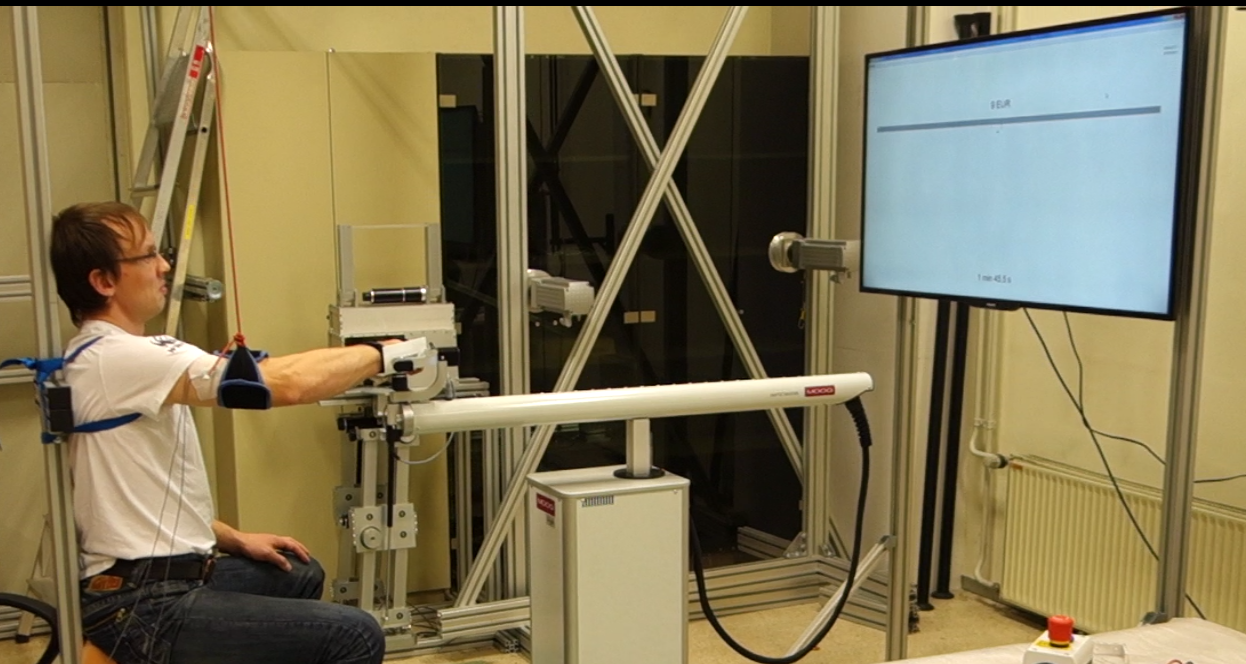
\includegraphics[width=\linewidth]{images/UnifyingTwoPhenomena.png}
\caption{Experimental setup to understand how humans optimize arm reaching motions when the supportive hand contact has to be reached in order to maintain postural balance. The task of the subject was to obtain as high reward as possible in the given time by hitting a target on the virtual wall without knowing its actual size. In effect, the subjects had to find the optimal balance between precision, speed of motion and its cost in order to maximise the reward. To amplify the effect of cost of motion, haptic robot emulated a viscous media through which the subject had to move the hand.
}
\label{fig:UnifyingTwoPhenomena}
\end{figure}





%\subsection{•}-body controllers}
\section{Whole-body controllers}

The overall objective of the work on controllers is to provide a control architecture dedicated 
to humanoid robots involved in personal/service applications that imply physical interactions,
 \textit{i.e.} contacts, with the environment. Such a control architecture is a requirement to bridge 
 the existing gap between state-of-the-art methods in humanoid robots control and real-world
applications. This gap is, at the control level, mostly due to two factors. The first one is the intrinsic 
complexity of the robotic system itself as well as the complexity of the environment. This complexity induces uncertainties in the
knowledge of the models. The second factor is related to the complexity of the decision making process which, in real world applications, can be very challenging especially when dealing with missions implying the sequenced and/or parallel realization of complex actions by the robot. The combination of those two complexities results in third factor, related to the large computation  times necessary to take control decisions.
The state-of-the-art methods in humanoid robot are mostly two: pure motion planning and pure reactive control.
 The former tries to solve off-line the overall decision-making process but the actual action execution phase (typically open-loop) tends to fail because of the ``complexity and uncertainty'' factors. The latter succeeds in overcoming the ``complexity and uncertainty'' factor mostly
thanks to the use of feedback. However the proposed solutions are only locally optimal and the overall
decision-making process cannot be addressed in the most general cases (\textit{i.e.} without scripted scenarios).
The path followed by the CoDyCo project to achieve both globally optimal and locally feasible control
policies is based on a control architecture featuring two intertwined levels. The first one is the central node of
the work described here: given a set of elementary operational tasks to achieve and their respective importance, it
provides a framework to compute the torques to be produced by the actuators at each time in order to achieve
at best the prescribed set of elementary tasks given some constraints acting on the system (limits, saturations,
local obstacles, contacts...). We call this level the ``local controller'' level. The second level directly impacts the objectives to be achieved by the local controller, temporally
sequences and parametrizes the use of elementary operational tasks in order to achieve some complex goal
(\textit{e.g.} ``grabbing an object on a table while standing and balancing using several contact points'') in a globally
optimal fashion. We call this level the ``global control policy'' level. 


%\subsubsection{Formulating and solving the local control problem}
\subsection{Formulating and solving the local control problem}

The work performed on formulating  and solving the control problem has led to the definition of what a task can be considered to be in the context of the reactive formulation of a multi-task whole body control problem. Among the different characteristics of a task (physical frame, task variable, forward model, desired target trajectory, local controller, priority), the notion of task priority has been largely modified with respect to the classical lexicographic task ordering met in the robotics literature and which is particularly appropriate for cascade resolution approaches such as the one recently proposed in \cite{escande2012}. A partial order has been defined such that task priorities can be described for any pair of task $i$ and $j$. This leads to a richer formulation which includes the original one but is also particularly appropriate for describing task insertion and removal processes as well as priority switching between tasks. Furthermore, this new prioritization paradigm provides a unique way of defining strict and soft hierarchies between tasks. Associated to this work, the notion  of generalized task projector has been introduced. Each task is associated to a projector which is built based on the tasks priorities. The interest of this projector is that it filters the joint space motion associated to a task so that all priorities are respected, being them soft or strict.

The control problem has been formulated as an LQP \cite{Salini-2011-ID348} which can be solved by any convex optimization solver dealing with linear constraints. Despite the task hierarchy, the introduction of a generalized task projector per task allows to solve only one LQP. This can be done by introducing as many virtual joint space variables as the number of tasks and using the generalized projector of each task in the expression of the constraints. The resulting problem can be solved by standard convex optimization tools and the cost of introducing virtual joint space variables is compensated for by the fact that only one optimization problem has to be solved. Details regarding this work, so-called Generalized Hierarchical Control (GHC), are provided in \cite{liuGHC2015} and a humanoid implementations is described in \cite{LiuAutRobSpecIssue2015}. 

A more classical hierarchical controller has also  been derived and is the one currently in use on the real robot \cite{DelPrete-2014-ID267}, \cite{noriFrontiers2015} and is described in the next section related to validation scenarii for the CoDyCo project.\\

We also started to investigate scenarios where the robot is interacting with the environment through rigid and non-rigid contacts. Assuming that no information is \textit{a priori} available regarding the nature of the contact surface, a first control strategy has been proposed in \cite{LiuIROS2015} where the desired contact force is adapted online as a function of the velocity of the contact point. Indeed, the risk with an unknown contact surface is to assume that it will almost instantaneously provide the required contact force to maintain the robot balance. If the surface is non-rigid, the contact point will actually move while being pushed and stable support forces will only be provided to the robot once the contact is properly established. The goal of the adaptation of the desired value for the contact force is to accelerate the attainment of a stable contact force supporting the robot. The desired trajectory for the center of mass of the robot is also adapted to account for the non-rigidity of the contact surface. One of the advantages of this approach is that it does not actually requires the knowledge of the contact surface impedance. Figure~\ref{fig:LIU_IROS_2015} provides a view of the types of considered scenarii and the structure of the considered controller. In this work, the local control problem is solved using the solver described in \cite{salini2012} rather than the one developed in \cite{liuGHC2015}. This choice is related to the fact that the computation cost of the GHC approach remains important and is too high to be actually used in a real-time reactive control architecture for a humanoid robot.

\begin{figure}[h!]
\centering
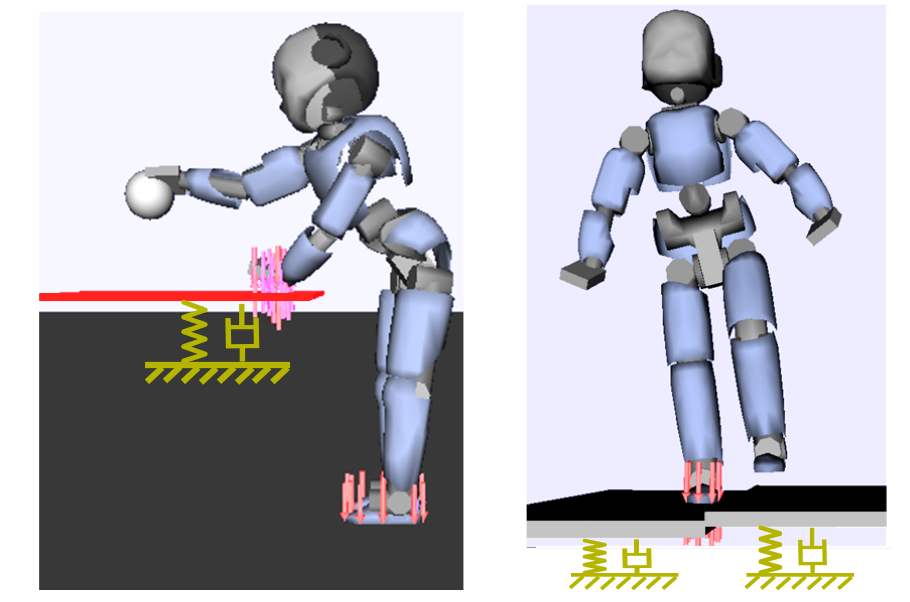
\includegraphics[width=0.8\linewidth]{images/LIU_IROS_2015}\\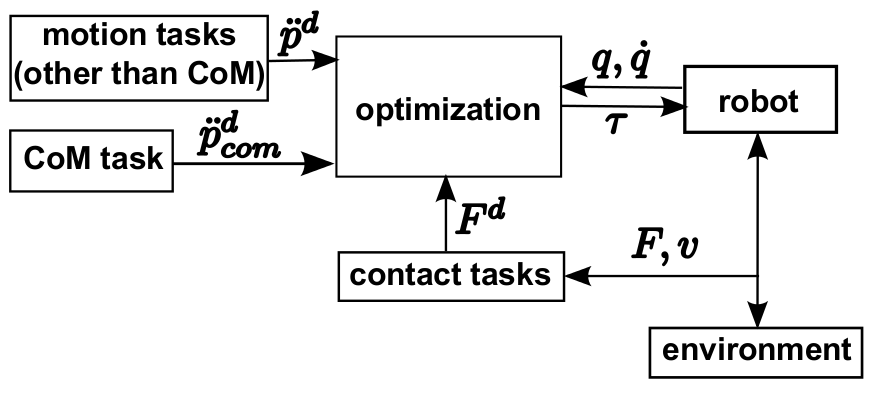
\includegraphics[width=0.8\linewidth]{images/LIU_IROS_2015_bis}
\caption{Scenarios of interaction with a non-rigid environment (\textit{top}). Structure of the adaptive control architecture (\textit{left}).}
\label{fig:LIU_IROS_2015}
\end{figure}

%\subsubsection{Bootstrapping and validating the control approach in rigid world and compliant cases}
\subsection{Bootstrapping and validating the control approach in rigid world and compliant cases}

In coordination with the local controller, we also have explored the contribution of MPC (Model Predictive Control) approaches to handle the postural balancing problem under varying contact conditions. The hybrid nature of the problem, where varying contact conditions can be accommodated either by adapting the internal forces distribution given a set of contact or by modifying the set of contacts itself, requires control approaches where the desired task trajectories performed through the local, reactive, whole-body controller have to be optimally planned ahead of time in order to provide robust behaviors. The contributions in this domain are mostly related to the work of A. Ibanez \cite{ibanez2013}, \cite{ibanez2014-icra} and \cite{ibanez2014-ark}. The originality of theses contributions lies in:
\begin{itemize}
	\item an augmented ZMP (Zero Moment Point, \cite{vukobratovic2004zero}) model including external forces exerted directly on indirectly on the center of mass;
	\item a distributed optimization approach that provides a way of generating reference trajectories for the center of mass representing a good compromise given some antagonistic balance and task;
	\item a non scripted foot step placement optimization.
\end{itemize}

As a  continuation of these works, in order to compute optimal time, duration and position of footsteps along with the center of mass trajectory of a humanoid, a novel mixed-integer model of the system is introduced in \cite{ibanezIROS2014}. The introduction of this model in a predictive control problem brings the definition of a Mixed-Integer Quadratic Program, subject to linear constraints. Simulation results demonstrate the simultaneous adaptation of the gait pattern and posture of the humanoid, in a walking activity under large disturbances, to efficiently compromise between task performance and balance. In addition, a push recovery scenario displays how, using a single balance-performance ratio, distinct behaviors of the humanoid can be specified. Results have been obtained in simulation\footnote{A video associated to this work can be found \href{http://pages.isir.upmc.fr/~padois/website/fichiers/videos/ibanez\_IROS2014.mp4}{here}.} and are being implemented on the TORO robot developed at DLR. Two simple and novel approaches to solve for 3D locomotion with multiple non-coplanar contacts have are also being explored in \cite{perrin2015}. Both formulations use model predictive control to generate dynamically balanced trajectories with no restrictions on the center of mass height trajectory. The first formulation treats the balance criterion as an objective function, and solves the control problem using a sequence of alternating convex quadratic programs, while the second formulation considers the criterion as constraints to the problem, and solves a succession of convex quadratically constrained quadratic programs. Preliminary results have been obtained in a scenario where a hand contact on a vertical wall is used to improve balance. A staircase climbing scenario has also been studied.\\

Bootstrapping between the local controller and a more global reasonning approach also lies in the capability to incrementally learn and adapt the models used for control.
Thus, we continued research in inverse dynamics model learning in situations with contacts. A mixture of experts approach combined with
Gaussian Processes was proposed in \cite{Calandra_ICRA15}, to learn the torque contributions due to contact exploiting the iCub's tactile and force/torque sensors. This approach was evaluated on the iCub robot, where the learned model accurately predicts contact forces, is robust to changes in the environment and outperforms existing analytic dynamic models that make use of force/torque sensor data. The interest in the use of such learned models over analytical ones lies also in the fact that learned models do not require a spatial calibration of the skin taxels, a procedure that in complex robots such as iCub is often prone to errors that significantly impact the torque estimation \cite{DelPrete2011}.
An exemplary task is illustrated in Figure~\ref{fig:exp3:icuparis_experiment_bars} 
when obstacles are introduced on both sides of a planned circular motion.
In Figure~\ref{fig:exp3:gating}, it can be seen that the mixture-of-experts recognizes the presence of the two different contacts and opportunely active the corresponding expert to compensate for the contact.
As a result, the torques predicted from this approach (red curve) closely follow the ground truth (blue curve) and outperform the analytic model (green curve).
%Further details can be found in \cite{Calandra_ICRA15}. 

	\begin{figure}[t]
		\begin{minipage}{.43\linewidth}
			\centering
			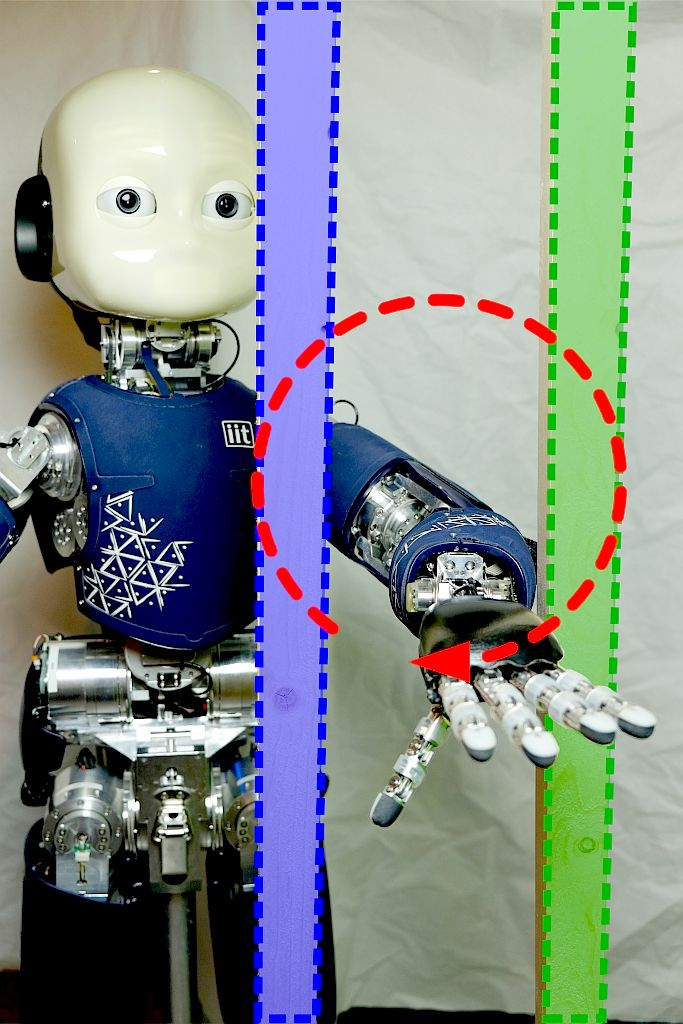
\includegraphics[width =.94\linewidth]{images/iCubParis02_Double_Contact}
			\caption{The robot performs a circle with its left arm. 
			The forearm collides alternatively with the left, the right or both contacts.}
			\label{fig:exp3:icuparis_experiment_bars}
		\end{minipage}	
		\hfill
		\begin{minipage}{.52\linewidth}
			\centering
			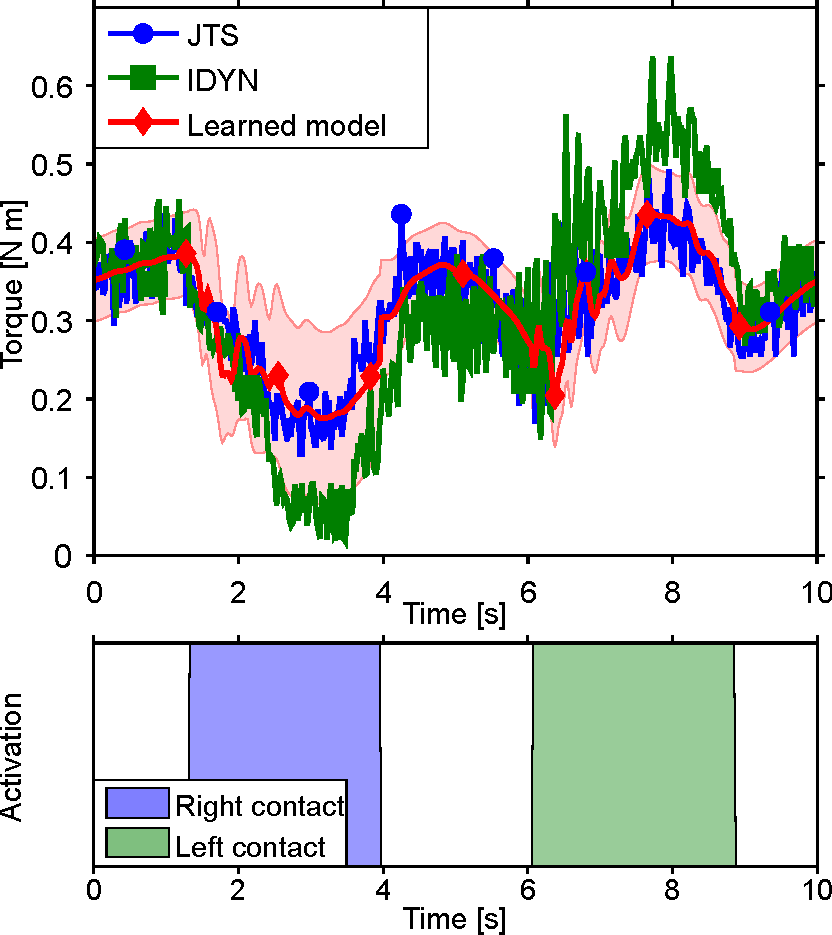
\includegraphics[width=.89\linewidth]{images/exp3_both}
			\caption{Prediction of torques with multiple contacts and the corresponding activation of the gating network.
			%Various models are shown, but individually, none of them correctly capture the dynamics of the system. 
			Our mixture-of-experts model combines the learned single-contact models into a multiple-contact model which outperform the analytic approach.
			}
			\label{fig:exp3:gating}
		\end{minipage}	
        %\figspace
	\end{figure}
	
\subsection{Validation scenarios}

This section presents the whole-body control framework implemented on the humanoid robot iCub for one foot balancing and motion control. This framework ensures a degree of compliance for the multi-body system, which allows for safe human robot interaction.

\subsubsection{System modelling}
The system dynamics are characterized by the following  differential equations:

\begin{eqnarray}\label{eq:dyn}
\label{eq:dynNoContacts}
M(q) \dot{\nu} + h(q, \nu) - J^\top(q) f  &=&
{S} \tau \mbox{,}\\
\label{eq:contact}
 J(q) \dot{\nu} + \dot{J}(q, \nu) \nu &=& 0 \mbox{,}
 \end{eqnarray}

\noindent
where $q \in SE(3) \times \Rv{n}$ represents the configuration of the free floating system,
 which is given by the
pose of a base-frame and $n$ generalized coordinates $q_j$ characterizing the joint angles.
% (includes both $q_j \in \Rv{n}$ and the
% floating-base
The vector $\nu \in \Rv{n+6}$ represents the robot velocity
(it includes both $\dot{q}_j \in \Rv{n}$ and the linear and angular velocity of the base-frame $v_b \in \Rv{6}$), the system acceleration is denoted as $\dot \nu$,
the derivative of $\nu$, the control input
$\tau \in \Rv{n}$ is the vector of joint torques, $M \in \R{(n+6)}{(n+6)}$ is the mass matrix, $h \in \Rv{n+6}$ contains both
gravitational and Coriolis terms, $S \in \R{n}{(n+6)} := (0_{n\times 6}, I_n)^\top$ is the matrix selecting the actuated degrees of freedom, $k$ is the number of constraints acting on the system, $f \in \Rv{k}$ are the generalised forces associated to the constraints, and $J \in \R{k}{(n+6)}$ is the constraint Jacobian \eqref{eq:contact}.


\subsubsection{Problem statement}

The control objective is the asymptotic stabilization of a desired centroidal dynamics \cite{Orin2013}. Let $H$
denote the centroidal momentum of the robot. Then, the time derivative of $H$ is equal to the summation of the external wrenches acting on the multi-body system. By expressing the centroidal momentum with respect to the center of mass, we have:

\begin{eqnarray} 
    {\dot H}  =   X f + mg 
     = \begin{pmatrix} m \ddot{x} \\ \dot{H}_\omega  \end{pmatrix} \label{eq:constraintsSi}
\end{eqnarray}
where $m$ is the mass of the robot, $g \in \mathbb{R}^6$ is the gravitational acceleration, $\ddot{x} \in \mathbb{R}^3 $ 
is the acceleration of the center of mass, $H_\omega \in \mathbb{R}^3$ is the \emph{angular momentum} of the robot, and the matrix $X$ maps the contact wrenches on the center of mass.

The control objective is to find a control law for the inputs $\tau$ such that $x \rightarrow x(0)$ and $H_\omega \rightarrow 0$. This choice is sufficient for balancing purposes. Also, while achieving this control objective, the system shall have a degree of compliance.

\subsubsection{The control strategy}
The control strategy is composed of two steps. We first choose the external force $f$ such that $x \rightarrow x(0)$ and $H_\omega \rightarrow 0$. Then, we generate this force through the internal torques. Since iCub possesses more than six degrees-of-freedom, which are necessary to generate the contact force $f$, we choose the remaining control inputs so that to have compliance at the joint level.

\subsubsection{The choice of the contact force}

Being the matrix $X$ invertible, the contact force $f$ achieving the control objective may be chosen as follows:

\begin{multline} 
    \label{fd}
   f = -X^{\dagger}\left[k_d H + k_p\begin{pmatrix} x-x(0) \\ 0_{3\times1}  \end{pmatrix} + mg\right] \\ + \left( I - X^{\dagger} X \right) f_0, 
\end{multline}
 with $k_d$ and $k_p$ two positive constants and $f_0$ arbitrarily chosen to obtain a solution $f$ as similar as possible to a desired value.
 
 In order to keep the motion constraints satisfied, $f$ must satisfy some constraints, \textit{e.g.}, the contact forces
 must belong to the associated friction cones. In general, the contact constraints can be represented by inequalities of the 
 form $Cf < d$, with the matrix $C$ and the vector $d$ properly chosen. Then, we choose the contact wrench  as fallows:

\begin{subequations} \label{eq:TSID}
\begin{align}
\label{eq:torquesTSID}
  f = & \argmin_{  \xi \in \mathbb{R}^6} \|   \xi -   f_d\|^2 \\
\label{eq:dynTSID}
& \mbox{s.t.}  \quad C\xi < d, 
%\label{eq:motionTSID}
% J_i \ddot{  q} + \dot{J}_i \dot{  q} & = \ddot {  x}_i^*, \qquad i = 1, \dots, N -1
\end{align}
\end{subequations}
with the desired wrench $f_d$ given by \eqref{fd}.

%
% \begin{eqnarray}
%     {\dot H}  & = &   { X}^*_{lf} f + mg = \begin{pmatrix} m \ddot{x} \\ \dot{H}_\omega  \end{pmatrix} \label{eq:constraintsSi}
%     % A & = & \begin{bmatrix} ^{com} { X}^*_{rf} & ^{com} { X}^*_{lf} \end{bmatrix}, \notag
% \end{eqnarray}
%
% Let us briefly recall how the force-control problem is solved in the Task Space
% Inverse Dynamics (TSID) framework
% proposed by \cite{delPrete2013} in the context of free floating robots.
% The framework computes the
% joint torques to match as close as possible a desired vector of forces at the contacts \eqref{eq:torquesTSID}
% while being compatible with the system dynamics \eqref{eq:dynTSID} and contact constraints
% \eqref{eq:contactTSID}:
%
% \begin{subequations} \label{eq:TSID}
% \begin{align}
% \label{eq:torquesTSID}
%   {\tau}^* = & \argmin_{  \tau \in \mathbb{R}^n} \|   f -   f^*\|^2 \\
% \label{eq:dynTSID}
% & \mbox{s.t.}  \quad M \dot{ \nu} + h - J^\top   f = S   \tau \\
% \label{eq:contactTSID}
% & \quad \quad J \dot{ \nu} + \dot{J}_c \nu  = 0
% %\label{eq:motionTSID}
% % J_i \ddot{  q} + \dot{J}_i \dot{  q} & = \ddot {  x}_i^*, \qquad i = 1, \dots, N -1
% \end{align}
% \end{subequations}
% \noindent
% where $f^* \in \Rv{k}$ is the desired value for the contact forces.
% %${  x}^*_i (q)$ is  is the desired value for some kinematics variables ${  x}_i (q)$ and $J_i = \partial x_i / \partial q$ is the associated Jacobian.
% Then we can exploit the null space of the force task to perform lower priority motion tasks.
% These tasks (indexed with $i$) are all expressed as the problem of tracking a given reference acceleration $\dot {\nu}_i^*$ for a
% variable ${x}_i$ differentially linked to $q$ by the Jacobian $J_i$.
% We impose that the force task has maximum priority in the task hierarchy.
% The final solution, i.e. the torques to be applied to the robot, are obtained by recursively solving a minimization problem similar to (\ref{eq:TSID}) in the null space of all the tasks with higher priorities.
% Assuming that the force task has maximum priority the solution is:
% \begin{equation} \label{eq:hyb_dyn}
%   \tau^{*} = -(J\bar{S})^\top   f^* + N_j^{-1} {\dot{v}}_1^* + \bar{S}^\top n,
% \end{equation}
% where $N_j^{-1} = M_j - M_{bj} M_j^{-1} M_{bj}^\top$, $\bar S = \mat{-M_{bj}^\top M_b^{-1} & I}^\top $ and the term ${\dot{v}}_1^*$ is computed solving the following recursion for $i =N$, $\dots$, $1$:
% \begin{equation}
% \begin{split}
% \dot{v}_i =& \dot{v}_{i+1} + (J_i \bar{S} N_{p(i)})^\dagger (\ddot{  x}_i^*-\dot{J}_i v + J_i (U^\top M_b^{-1} (h_b - J_{cb}^\top f) - \bar{S} \dot{v}_{i+1}))\\
% N_{p(i)} =& N_{p(i+1)} - (J_{i+1} \bar{S} N_{p(i+1)})^\dagger J_{i+1} \bar{S} N_{p(i+1)}, \\
% %N_{p(i)} =& I - \sum_{j=i+1}^{N}(J_j \bar{S} N_{p(j)})^+ J_j \bar{S} N_{p(j)},
% \end{split}
% \end{equation}
% where $U \in \mathbb{R}^{6 \times (n+6)}$ is the matrix selecting the floating-base variables, and the algorithm is initialized setting $\dot{v}_{N+1} = 0$, \mbox{$N_{p(N)}=I$}, $J_N = J$ and $\ddot{ x}_N = 0$.
% The implementation of this controller exploits the fact that we can compute \eqref{eq:hyb_dyn} with an efficient hybrid-dynamics algorithm.

\subsubsection{The choice of the joint torques}
The control input $\tau$ must generate the force $f$. The relationship between the contact wrench and the joint torques can be obtained by using the constraint equation along with the free-floating dynamics, \textit{i.e.} Eq. \eqref{eq:dyn}.
One can show that the torques generating $f$ are given by the summation of two terms, \textit{i.e.},
\begin{eqnarray}
        \label{tau}
        \tau = \tau_f + N \tau_0,
\end{eqnarray}
where $\tau_f $ ensures $f = f_d$, the matrix $N \in \mathbb{R}^{n\times n}$ is the null space projector of 
$JM^{-1}S$,
and $\tau_0$ is a vector that can be chosen at will. To obtain compliance at joint level, we choose $\tau_0$ similar to 
a gravity and external force compensation, plus a term of the form \[ -k(q_j - q_d),\]
which ensures  compliance at joint level.


% The control framework described in the previous section can be applied for a balancing task, while retaining the possibility of interaction with the environment.
% Instantaneous values for interaction forces at feet are computed to
% follow a prescribed center-of-mass trajectory ($x_{com}^d$) and to reduce angular momentum\footnote{Quantities are defined with a notation similar to \cite{Featherstone2008}}. A reference value  $\dot H_{com}^*$ for the total rate of change of spatial momentum (expressed at the center of mass) is computed as:
%
% \begin{eqnarray} \label{eq:hRef}
% {\dot H}^* (t) = {\dot H}_{com}^d (t) -  K_d^{h} \tilde{H}_{com} - \begin{bmatrix} K_p^{com} \left( \tilde{x}_{com} \right)\\ 0_{3\times1}  \end{bmatrix}
% \end{eqnarray}
%
% \noindent
% where $K_d^{h}$, $K_p^{com}$ are suitably defined gain matrices, $\tilde{(\cdot)}$ denotes the error with respect to the desired quantity, $H_{com}$  and $H_{com}^d = [m \dot{x}_{com}^{d\top}, 0_{1\times3}]^\top$ is the spatial momentum around the center of mass and its desired value, $x_{com}$ is the center-of-mass cartesian position, $x^d_{com}$ its desired value and $m$ is the total mass of the robot.
% The relation between external forces and ${\dot H_{com}}$ is given by the following equation:
% % At this point $f^*$ can be computed from ${\dot H_{com}}^*$
% % considering that the time derivative of the momentum equals the resultant of forces and torques if all
% % quantities are computed with respect to the center of mass:
% \begin{eqnarray}
%     {\dot H_{com}}  & = &   A f + f_g \label{eq:constraintsSi}\\
%     A & = & \begin{bmatrix} ^{com} { X}^*_{rf} & ^{com} { X}^*_{lf} \end{bmatrix}, \notag
% \end{eqnarray}
% where $f_g$ is the gravitational force and where the matrices $^{com} { X}^*_{(\cdot)}$  express the spatial forces acting on the left foot ($lf$) and right foot ($rf$) with respect to the center of mass.
% In literature these equations (derived from the Newton-Euler equations) have been presented in detail by
% \cite{Orin2013} under the name of \emph{centroidal dynamics}.
%
% Finally, the desired force $f^*$ can be computed as
%
% \begin{equation} \label{eq:minF}
%  f^* = \argmin_{f} \|  f  - f_0 \|^2  \qquad \mbox{s.t.} \qquad A f + f_g = {\dot H_{com}}^*,
% \end{equation}
% The solution of this optimization is given by:
% \begin{equation}
%  f^* = A^{\dagger} \left( {\dot H_{com}}^* - f_g \right) + (I - A^{\dagger} A)  f_0 ,
% \end{equation}
% \noindent
% where $f_0$ can be chosen to satisfy additional constraints on the forces.
%
% We also added, at the lowest priority level, a postural task. Reference accelerations for the joint variables are chosen as:
%
% \begin{equation} \label{eq:qRef}
% {\ddot q_j}^* (t) = {\ddot q_j}^d (t) - K_d^{q} \left( {\dot q_j} - {\dot q_j}^d (t) \right) - K_p^{q} \left( {q_j} - { q_j}^d (t) \right),
% \end{equation}
% where $K_p^{q}$ and $K_d^{q}$ are arbitrary positive-definite matrices
% This task acts in the null space of the task force as specified in Eq. (\ref{eq:TSID}).
% In the general case more tasks can be added between the highest priority one (force task) and the lowest priority one (postural task).

\subsubsection{Experiment}

\begin{figure}
\centering
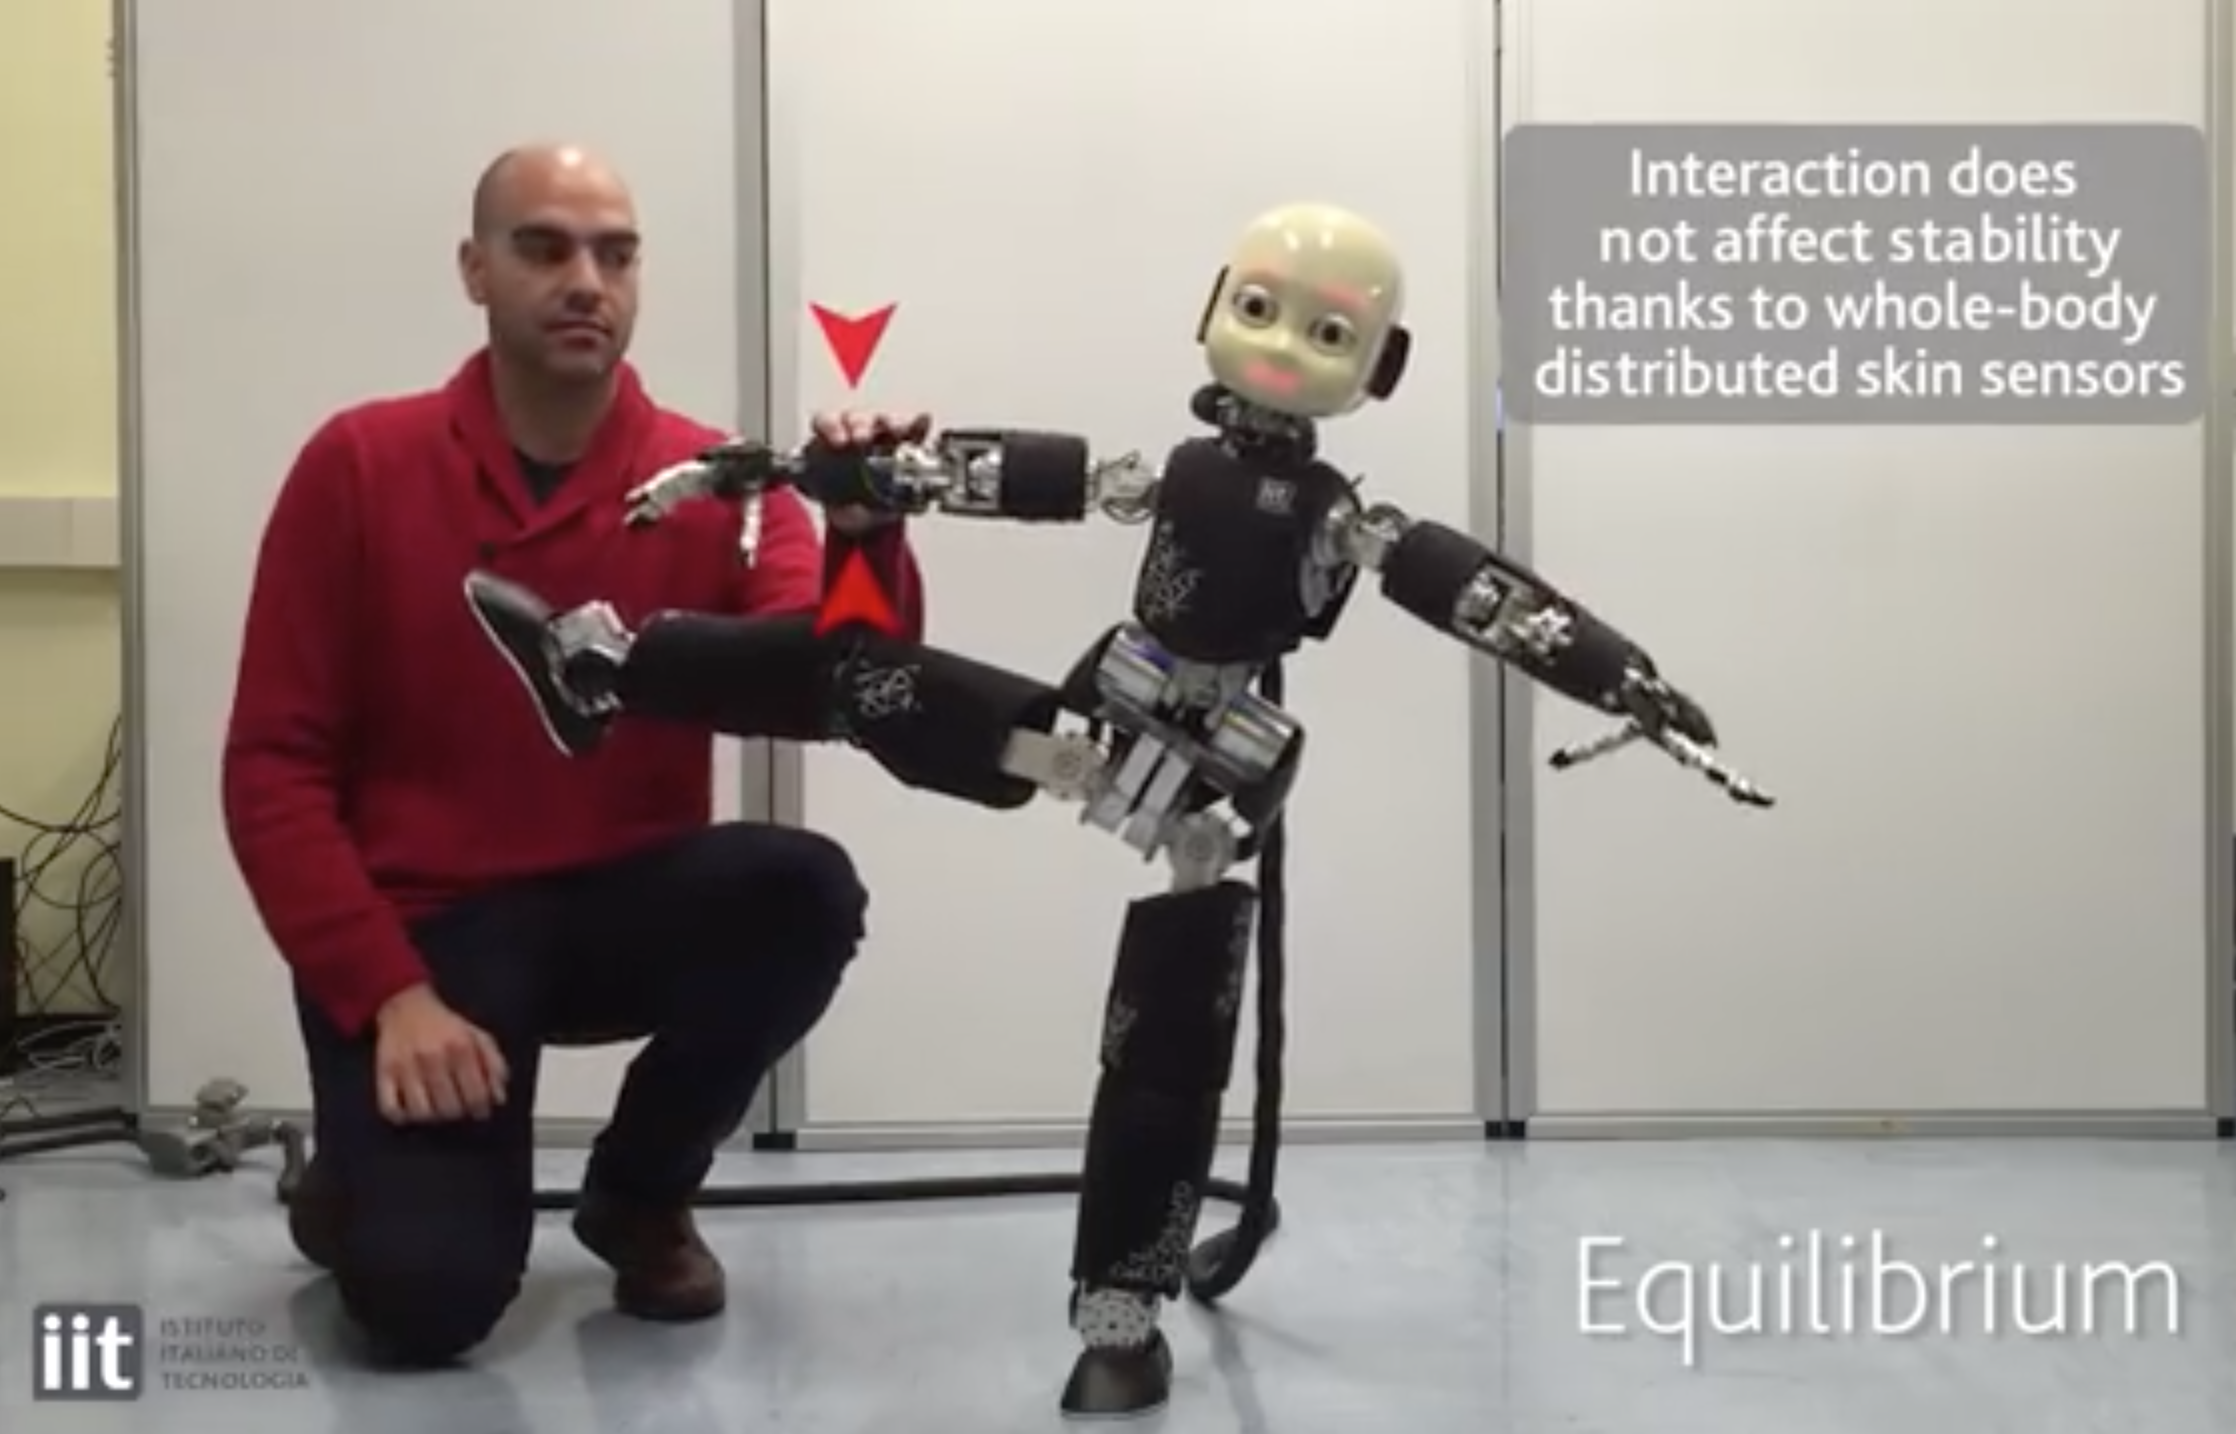
\includegraphics[width=0.9\columnwidth]{images/icubPicture} \\
\caption{Screenshot of the video showing the full experiment. iCub balances by controlling the foot wrench.
} \label{fig:snapshot}
\end{figure}

% \begin{figure}
% \centering
% \includegraphics[width=0.8 \textwidth]{images/twoSupportsSignals.pdf} \\
% \caption{Results of the double support experiment on planar contacts (left and right feet). The picture shows
% the time behavior of forces (top) and center of mass position (bottom) on the sagittal (blue) and transverse
% (green) axis. It is worth \replaced[id=jeg]{noting}{noticing} that forces should be proportional to center of mass accelerations and this
% is visible in the plot considering that accelerations are \replaced[id=jeg]{sinusoidal}{sinusoid} in counter phase with positions.
% \adnote{Add desired CoM trajectory and desired forces?} Rapid variations of the contact forces at the time $t \approx 2$, i.e. starting time, are due to
% the activation of the torque control.}
% \label{fig:twoSupportsForces}
% \end{figure}
%
% \begin{figure}
% \centering
% \includegraphics[width=0.4 \textwidth]{images/twoSupports.pdf}
% \includegraphics[width=0.4 \textwidth]{images/twoSupportsFRI.pdf}
% \caption{Results of the double support experiment on planar contacts (left and right feet). The left picture
% shows in three dimensions the feet contacts, the feet center of pressures, the forces at the feet and at the
% the center of mass during three instants: at two extrema of the sinusoid (red and blue) and in the middle of
% the sinusoid (green). Remarkably forces are maximum at the extrema when also accelerations are
% maximal. The right picture shows a close-up of of the feet with the trajectory of the center of pressure, an
% ellipse representing a Gaussian fit of the data points and three points corresponding to the position of the
% centers of pressure when at the two extrema of the sinusoid (red and blue) and in the middle of the sinusoid
% (green). \adnote{I found this figure hard to interpret, even after reading the caption, the RGB arrows/points are hard to see.}} \label{fig:twoSupports}
% \end{figure}
%
% \begin{figure}
% \centering
% 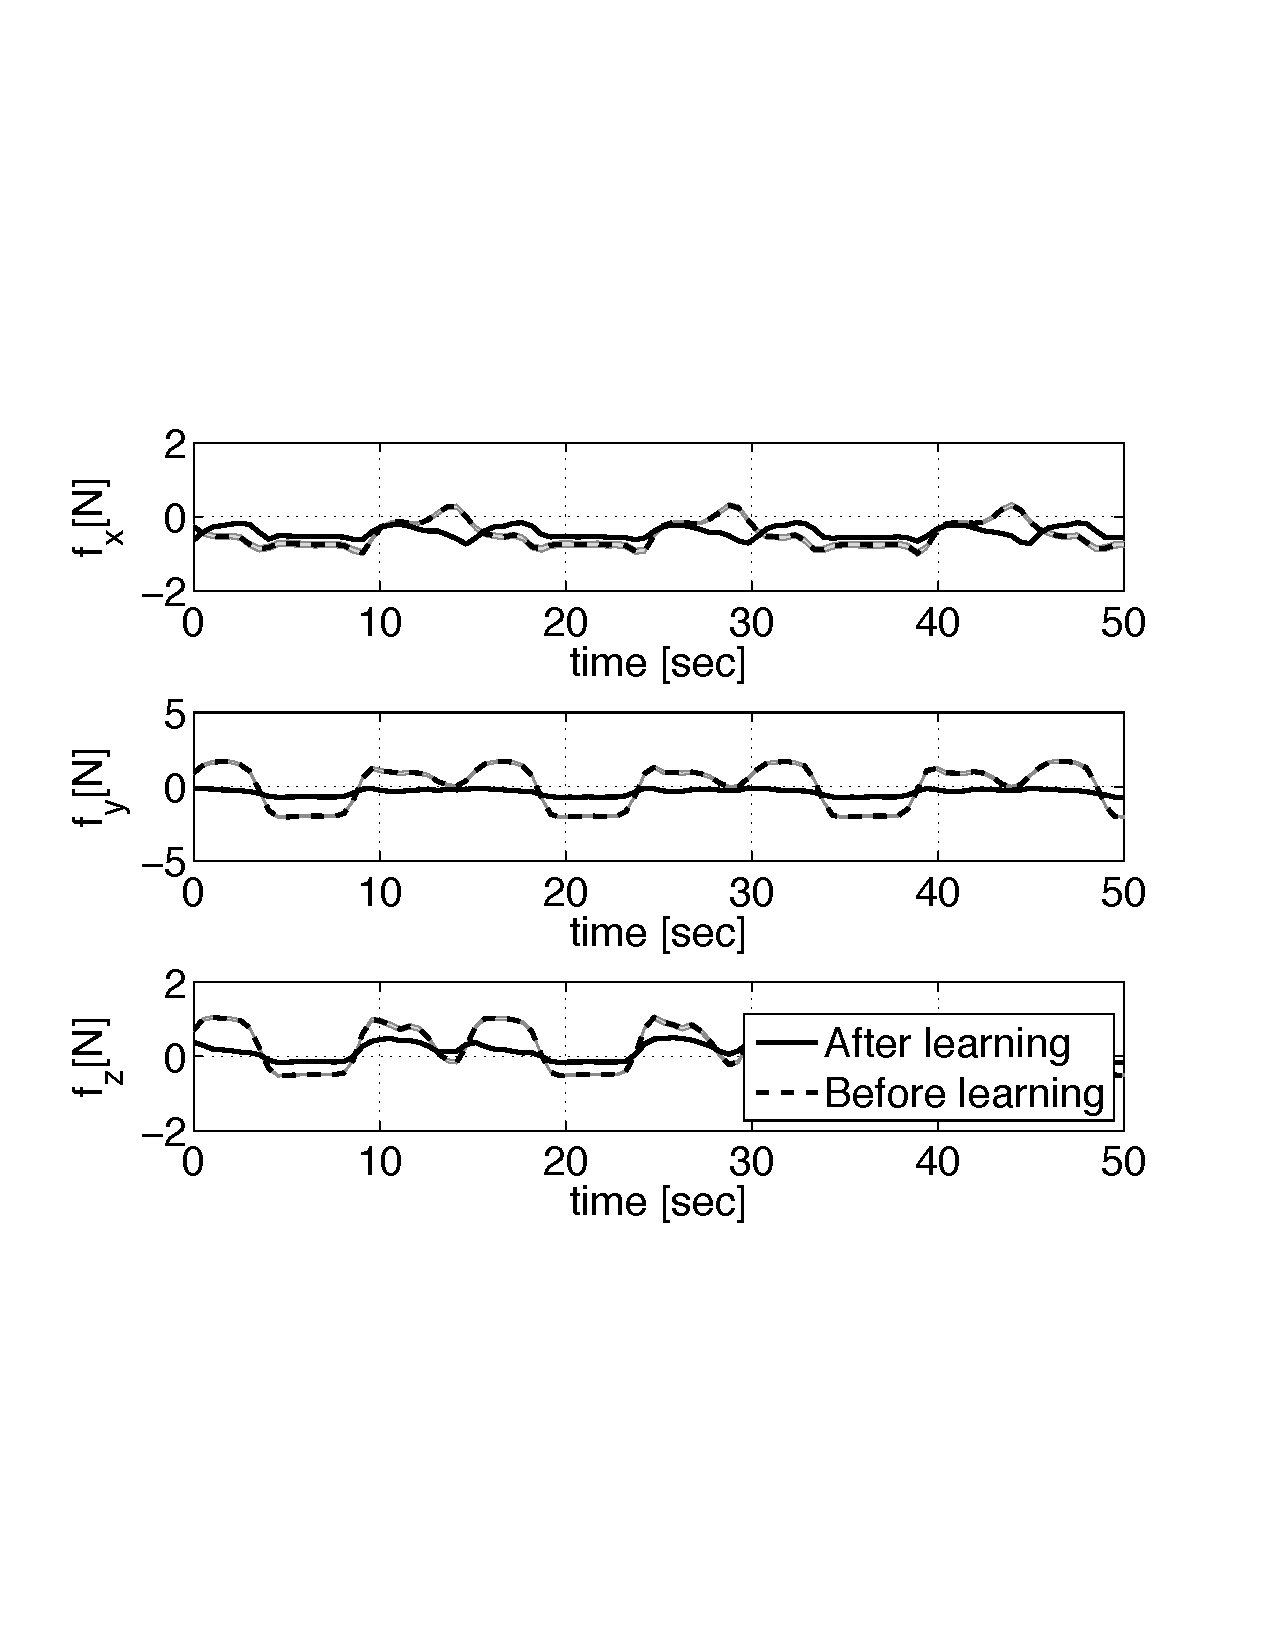
\includegraphics[width=0.8 \textwidth]{images/forces.pdf} \\
% \caption{Results of the double support experiment on four noncoplanar contacts (both feet and
% arms). The plots represent the evolution of the contact forces at the left (top) and right (bottom) arms when
% contact is established.} \label{fig:fourSupportsForces}
% \end{figure}
%
% \begin{figure}
% \centering
% \includegraphics[width=0.4 \textwidth]{images/fourSupports.pdf}
% \includegraphics[width=0.4 \textwidth]{images/fourSupportsFRI.pdf}
% \caption{Results of the double-support experiment on four noncoplanar contacts (both feet and
% arms). The left picture gives a three-dimensional view of the foot center-of-pressure positions together with
% the arm contact forces. Forces are represented in a color scale that goes from black (contact establishment)
% to blue (steady state) \adnote{I found the forces hard to interpret so I'd remove them since they are already in the previous plot}.
% The right picture gives a closeup on the foot center-of-pressure positions with an
% ellipse that represents the Gaussian approximation of its distribution. \adnote{Overall this figure is hard to read, so I suggest replacing
% it with a plot of the CoP.}} \label{fig:fourSupports}
% \end{figure}

We implemented the proposed control strategy on the iCub platform as illustrated in Figure~\ref{fig:snapshot}. The control framework is composed of two
loops. The inner loop is in charge of stabilizing \emph{desired} joint torques, while the outer loop is governed by 
Eq. \eqref{tau}. Both loops runs at the same frequency of 100 Hz. 

The experiment consists in two phases. In the first phase, we change the desired $q_d$ in order to generate 
\emph{internal} motions, which do not perturb the stability of the robot momentum thanks to the prioritization of tasks
described in the previous section. In the second phase, we apply external perturbations by interacting with the robot as illustrated in Figure~\ref{fig:footBalancing}. This 
interaction  results to be safe thanks to the compliance at joint level\footnote{A video of the experiment is available \href{https://www.youtube.com/watch?v=VrPBSSQEr3A}{here} for the interested reader.}.

For more detailed information and description of the system architecture (comprising torque and forces estimation and low level torque control) see \cite{noriFrontiers2015}.

\begin{figure}[h!]
\centering
{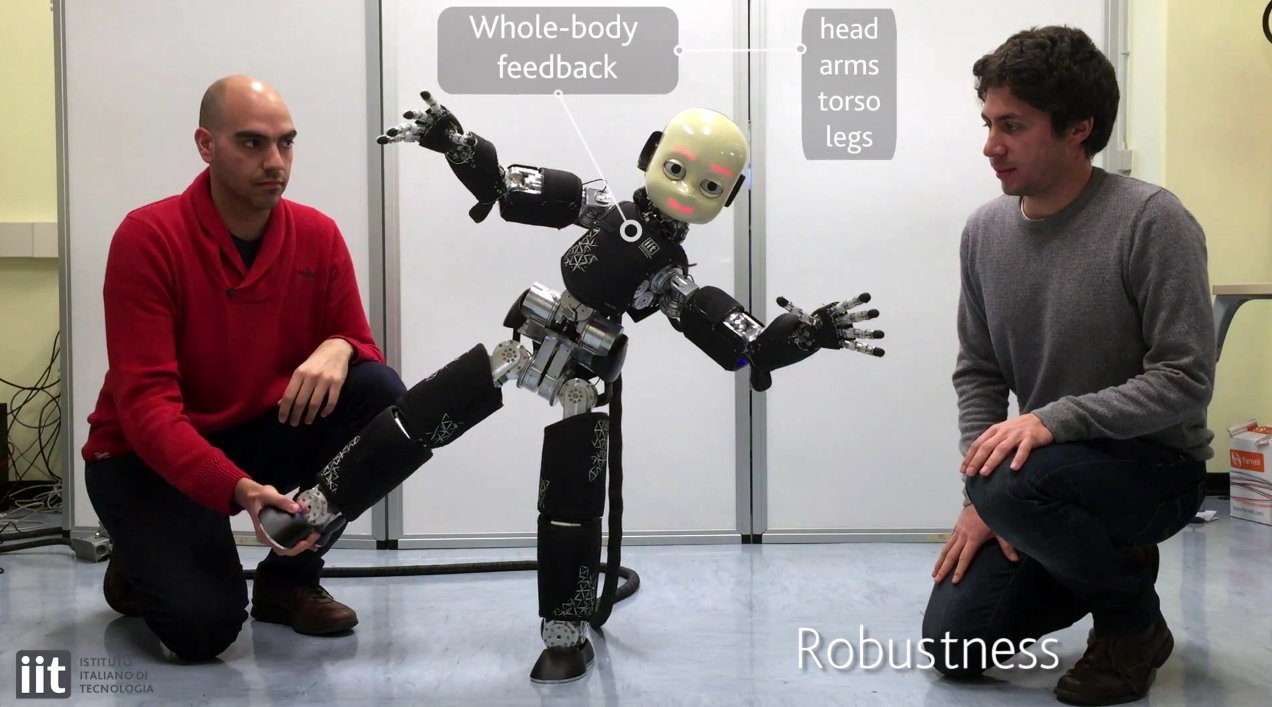
\includegraphics[width=\linewidth]{images/single_foot_balancing.jpg}}
\caption{The picture shows the iCub while performing compliant single foot balancing. Details on the controller can be found in \cite{Nori2015a}. A video of the task is available on \href{https://www.youtube.com/watch?v=SYVCbzGsBF4}{youtube}.}%\protect\footnotemark.}
\label{fig:footBalancing}
\end{figure}

%\footnotetext{\url{}.}

%\subsection{Learning}
\section{Learning}

The goal of the work on Learning in CoDyCo is to endow humanoid robots control architectures with the core abilities for the adaptation, generalization and self-improvement of both control laws and tasks that involve physical interaction with humans, and the environment. In this context, we propose learning approaches that work in conjunction with the control architecture devised in the presvious sectio  and rather complement analytical robotic approaches with on-policy learning than starting from scratch. A core idea behind this work is that Learning should complement classical approaches and not supersede them.

%\subsubsection{Inferring the Operational Space and Appropriate Controls with Multiple Contacts}
\subsection{Inferring the Operational Space and Appropriate Controls with Multiple Contacts}

%TUD
For controlling high-dimensional robots, most stochastic optimal control
algorithms use approximations of the system dynamics and of the cost function
(\textit{e.g.}, using linearizations and Taylor expansions). These approximations are
typically only locally correct, which might cause instabilities in the greedy
policy updates, lead to oscillations or the algorithms diverge. To overcome
these drawbacks, we added a regularization term to the cost function that punishes
large policy update steps in the trajectory optimization procedure. We applied
this concept to the Approximate Inference Control method (AICO), where the
resulting algorithm guarantees convergence for uninformative initial solutions
without complex hand-tuning of learning rates. 

\begin{figure*}[t]
  \begin{center}
  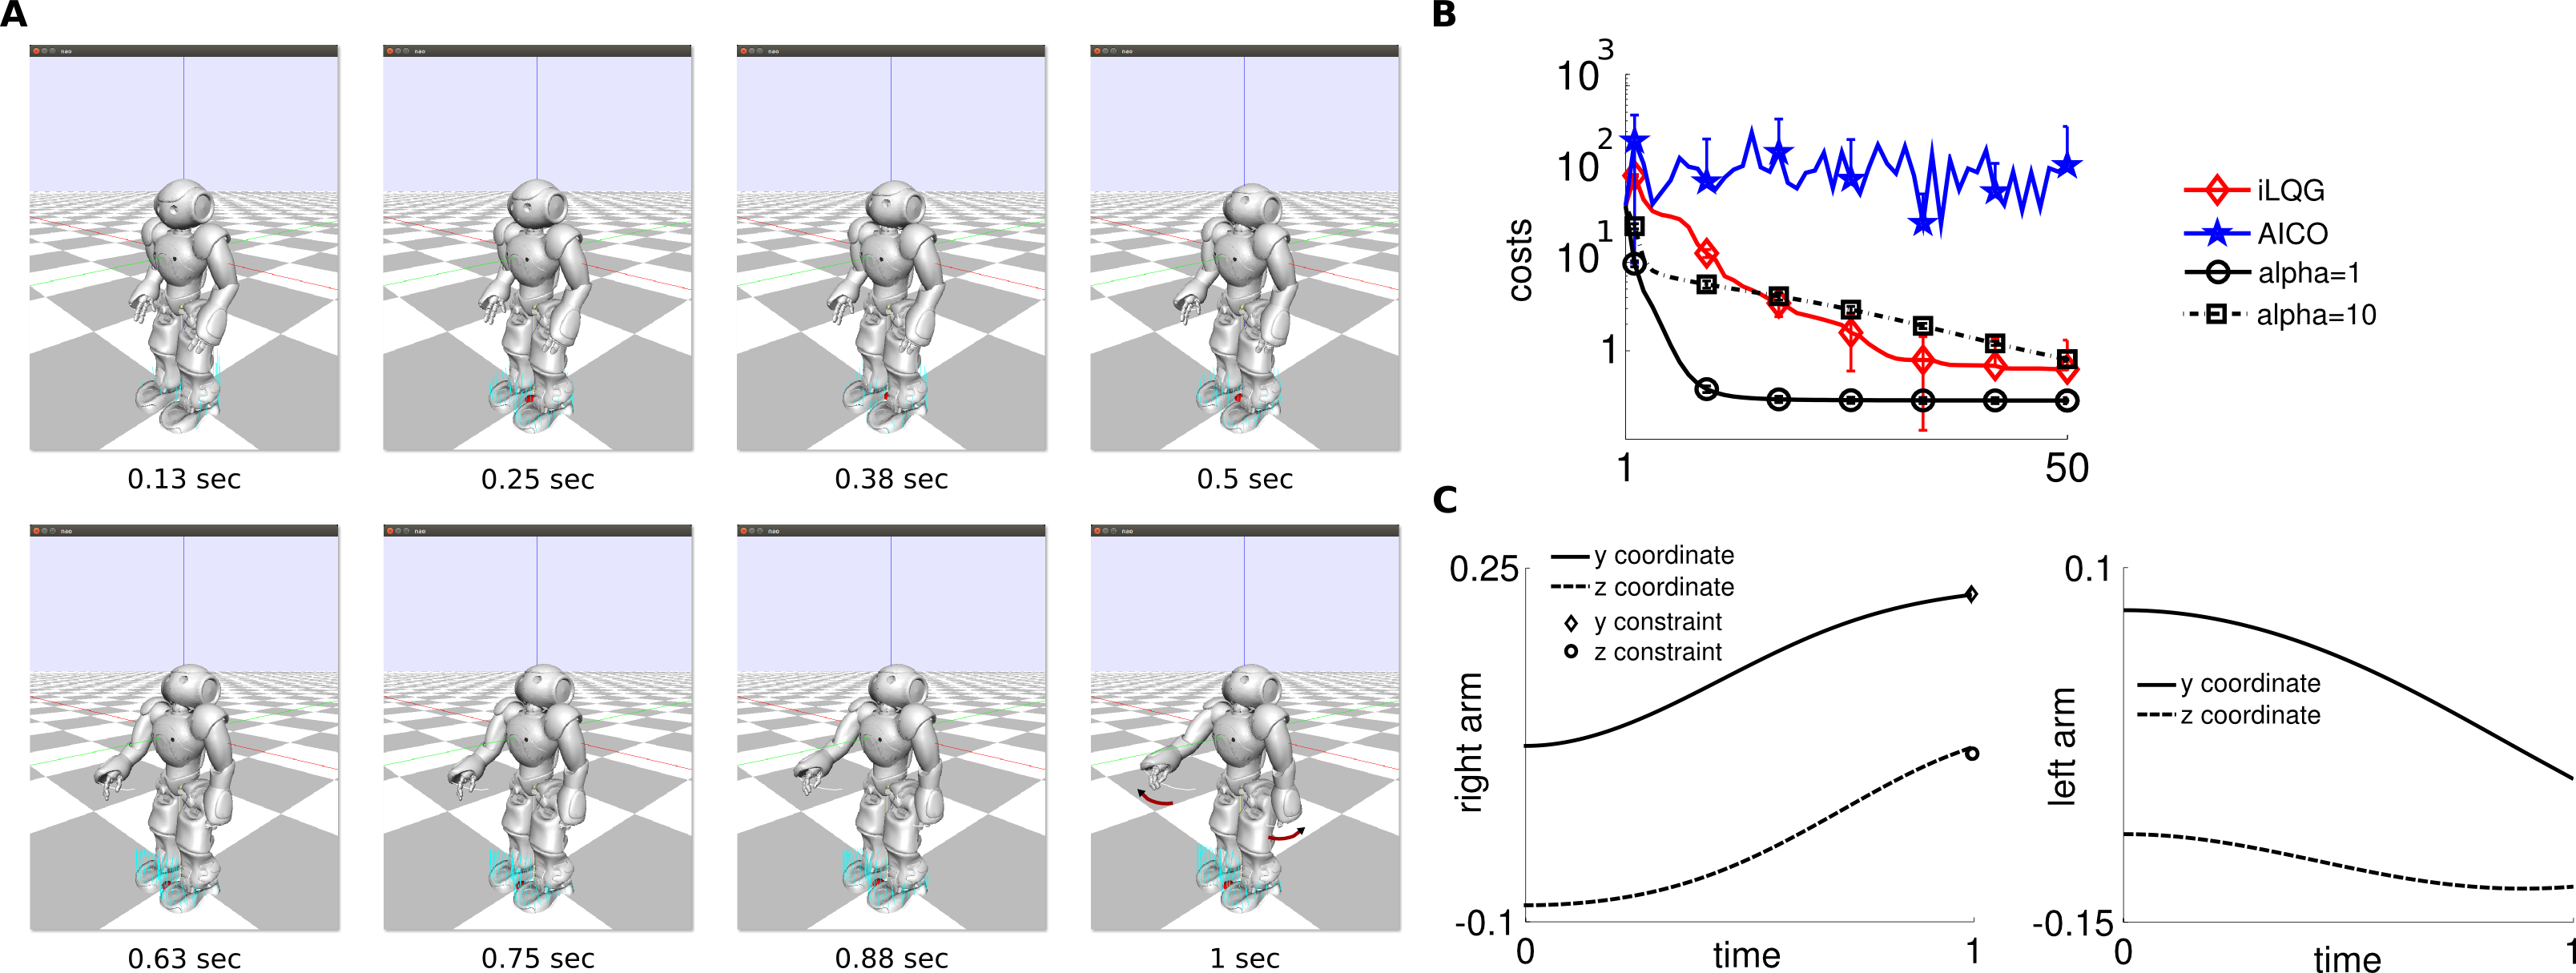
\includegraphics[width=\linewidth]{./sections/WP4/pics_elmar/NaoReachingTask.png}
  \end{center}
  \caption{Reaching task with the humanoid robot \textit{Nao}. The robot has to
reach  a desired end effector position with the right arm while maintaining
balance. Eight snapshots of the inferred movement are shown in (A). In (B), the
convergence of the costs of the optimization procedure is shown, where we
compare \textit{iLQG}, the standard implementation of AICO and the regularized
variant. The movement objectives for the right arm are shown in the left panel
in (C). To balance the robot lifts its left hand and bends the head back.}
  \label{fig:naoReachingTask}
  \end{figure*}

The new algorithm was evaluated on
two simulated robotic platforms. A robot arm with five joints was used for
reaching multiple targets while keeping the roll angle constant. On the humanoid
robot Nao, we show how complex skills like reaching (see Figure~\ref{fig:naoReachingTask}) and balancing can be
inferred from desired center of gravity or end effector coordinates. This work was published at 
the international conference on humanoid robots \cite{Rueckert2014}\footnote{Supplemental Matlab demo code is available \href{http://www.ausy.tu-darmstadt.de/Team/ElmarRueckert}{\textbf{online}}.}. 

%\subsubsection{Generalizing and Improving Elementary Tasks with Contacts}
\subsection{Generalizing and Improving Elementary Tasks with Contacts}

We aim to generate new skills from data, where elementary skills 
are acquired by imitation learning and transferred to novel situations using 
dynamic systems. To do so, we developed a novel representation of 
movement primitives that can be used for imitation learning from noisy observations.
Uncertainty of observed trajectories is explicitely modeled and used to generate new skills.
This movement representation has state-of-the-art capabilities in generalization, 
coupling between the degrees of freedom of the robot, and moreover, 
a time varying feedback controller can be derived in closed form. 
These features are partially illustrated in Figure~\ref{fig:promps}.
More details on this work can be found in \cite{Paraschos_NIPS_2013}.

\begin{figure}[!ht]
\centering
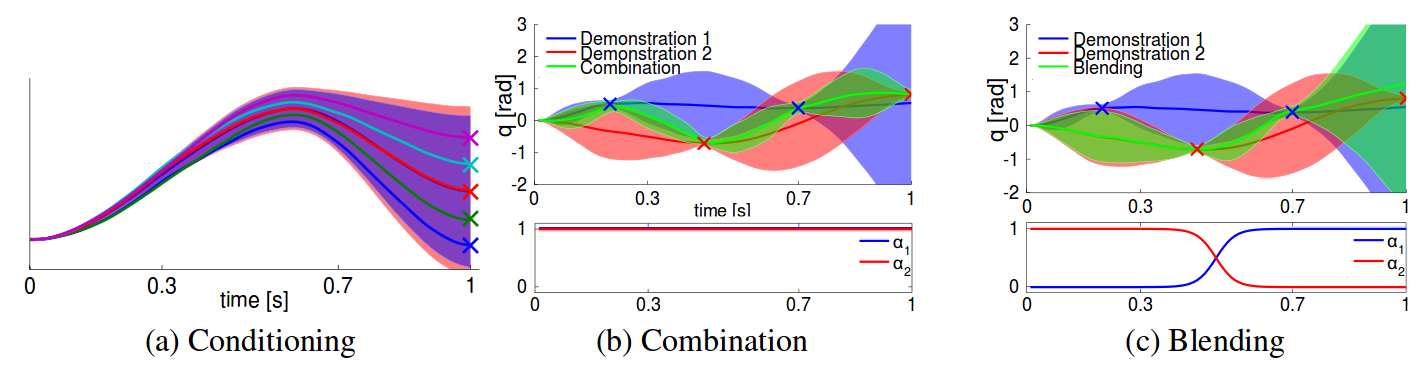
\includegraphics[width=\linewidth]{./images/ProMPs.png}
%\label{fig:subfig2}
 \caption{(a)
Conditioning on different target states. The blue shaded area represents the learned
trajectory distribution. We condition on different target positions, indicated by the $x$-markers. The
produced trajectories exactly reach the desired targets while keeping the shape of the demonstrations.
(b)
Combination of two ProMPs. The trajectory distributions are indicated by the blue and red
shaded areas. Both primitives have to reach via-points at different points in time, indicated by
the $x$-markers. We co-activate both primitives with the same activation factor. The trajectory
distribution generated by the resulting feedback controller now goes through all four via-points.
(c)
Blending of two ProMPs. We smoothly blend from the red primitive to the blue primitive. The
activation factors are shown in the bottom. The resulting movement (green) first follows the red
primitive and, subsequently, switches to following the blue primitive.
}
\label{fig:promps}
\end{figure}

The advent of robots in our every day life can only be accomplished with
reliable mechanisms for movement generation.  Movement Primitives (MP) are a
well-established approach for representing modular and re-usable robot movement
generators that can be composed into complex movements.  An easy-to-learn
representation of the primitive is, additionally, the key of recent imitation
and reinforcement learning successes. Current MPs approaches offer viable
properties such as concise representations of the inherently continuous and
high dimensional space of robot movements, generalization capabilities to novel
situations, temporal modulation of the primitive, sequencing of primitives,
coupling between the degrees of freedom of the robot, and controllers for real
time execution. However, no single MP framework exists that offers all these
properties.  We extended previous results on modeling stochastic movements \cite{Paraschos2013,Paraschos2013a}. 

\definecolor{light-gray}{rgb}{0.91,0.9,0.88}

\newcommand{\hockeyImLabel}[3]{%
\begin{tikzpicture}
\node[  anchor=south west,inner sep=0,%
        draw=gray,%
        %left color=gray,right color=white%
        %fill=light-gray%
] (image) at (0,0){
\includegraphics[width=0.29\textwidth]{#1}};
\begin{scope}[x={(image.south east)},y={(image.north west)}]
    %\draw[help lines,xstep=.1,ystep=.1] (0,0) grid (1,1);
    %\foreach \x in {0,1,...,9} { \node [anchor=north] at (\x/10,0) {0.\x}; }
    %\foreach \y in {0,1,...,9} { \node [anchor=east] at (0,\y/10) {0.\y}; }
    \node [fill=white,opacity=0.6,above right,font=\large] at (0.01,0.01) {#2};
    \node [fill=white,opacity=0.6,below left,font=\large] at (0.99,0.99) {#3};
\end{scope}
\begin{scope}[x={(image.south east)},%
              y={(image.north west)},% 
              on background layer]
    %\path[fill=light-gray] (0,0) rectangle (1,1);
    \path[outer color=light-gray,inner color=white] (0,0) rectangle (1,1);
    \draw[gray,opacity=0.15,xstep=.1,ystep=.1] (0,0) grid (1,1);
\end{scope}
\end{tikzpicture}%
}

\begin{figure*}
\centering
\hockeyImLabel{./sections/WP4/pics_alex/Setup_tr_sm.png}{$a$}{Setup}
\hockeyImLabel{./sections/WP4/pics_alex/Distances_tr_sm}{$b$}{Distance}
\hockeyImLabel{./sections/WP4/pics_alex/HockeyAngle_tr_sm}{$c$}{Angle}

\vspace{0.2em}

\hockeyImLabel{./sections/WP4/pics_alex/Joint_tr_sm}{$d$}{Union}
\hockeyImLabel{./sections/WP4/pics_alex/Combined_tr_sm}{$e$}{Combination}
\hockeyImLabel{./sections/WP4/pics_alex/Joint-LeftRight_tr_sm.png}{$f$}{Conditioning}

\caption{Robot Hockey. The robot shoots a hockey puck. We demonstrate ten straight
shots for varying distances and ten shots for varying angles. The
pictures show samples from the ProMP model for straight shots ($b$)
and angled shots ($c$). Learning from the union of the two data sets yields a model
that represents variance in both, distance and angle ($d$). Multiplying
the individual models leads to the combined a model that only reproduces shots
where both models had probability mass, in the center at medium distance
($e$). The last picture shows the effect of conditioning on only left
and right angles ($f$).}
\label{fig:Robot-Hockey}

\end{figure*}

We incorporated all the desirable properties 
current approaches offer into a single framework and, additionally, we 
introduced new operations on the primitives, such as continuous blending and
co-activation of multiple primitives.  Most importantly, in this approach, the
novel co-activation operator is capable of solving multiple tasks concurrently as illustrated in Figure~\ref{fig:Robot-Hockey}.
Furthermore, our approach is capable of reproducing exactly the demonstrated
variability of the movement and the coupling between the degrees of freedom of
the robot.  In this approach, called Probabilistic Movement Primitives (ProMPs) \cite{Paraschos2013,Paraschos2013a},
we derived all operations in closed form. In order to use the ProMPs for online
feedback control, we also derived a stochastic feedback controller that
reproduces exactly the encoded primitive. We evaluated and compared this approach
on several simulated and real robot scenarios.

Probabilistic movement primitives are a promising approach for learning,
modulating, and re-using movements in a modular control architecture.  To
effectively take advantage of such a control architecture, ProMPs support
simultaneous activation, match the quality of the encoded behavior from the
demonstrations, are able to adapt to different desired target positions, and
efficiently learn by imitation. ProMPs meets all of the aforementioned
requirements.  The desired trajectory distribution of the
primitive is parametrized by a hierarchical Bayesian model with Gaussian distributions. The
trajectory distribution can be obtained from demonstrations and 
simultaneously defines a feedback controller which is used for movement
execution. Currently, we are investigating extensions of the ProMPs framework 
to tasks that involve 
contacts with the environment. In addition, we started to investigate the improvement of elementary skills encoded in ProMPs with 
reinforcement learning, where a conference paper was submitted for review.

%\subsubsection{Learning the Prioritization of Tasks}
\subsection{Learning the Prioritization of Tasks}

We have been leading research on computed torque control leveraging low-gain control. 
In computed torque control, robot dynamics are predicted by dynamic models.
This enables more compliant control, as the gains of the feedback term can be
lowered, because the task of compensating for robot dynamics is delegated from
the feedback to the feedforward term.  We already showed that Gaussian Process
regression is an effective method for learning computed torque control, by
setting the feedforward torques to the mean of the Gaussian Process.  During
the second year of the project, we extended this work by also exploiting the
variance predicted by the Gaussian Process, by lowering the gains if the
variance is low \cite{Albertoetal14}.  This enables an automatic adaptation of
the gains to the uncertainty in the computed torque model, and leads to more
compliant low-gain control as the robot learns more accurate models over time.
On a simulated 7-DOF robot manipulator, we demonstrated how accurate tracking
can be achieved, despite the gains being lowered over time, which is illustrated in Figure~\ref{fig:meanvariance}.\\

\begin{figure}
  \centering
  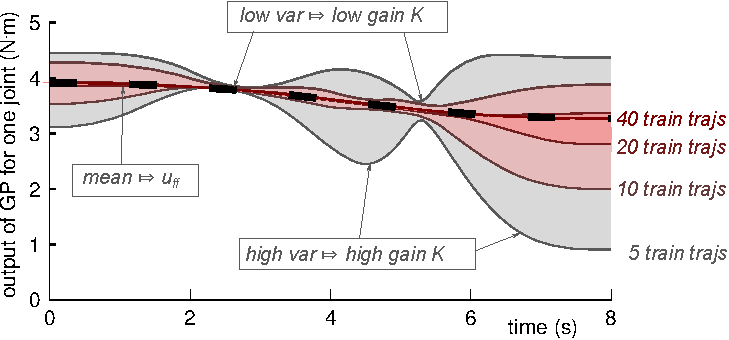
\includegraphics[width=\linewidth]{images/meanvariance.pdf}
  \caption{Mean and variance of the Gaussian process ($\mu \pm 2\sigma$) on
    the same test trajectory of 8 seconds, after having been trained with 5,
    10, 20 and 40 training trajectories. With an increasing number of training
    data, the mean of the GP approaches the true function (black dashed
    line). The known values for uff are plotted as a black dotted line.}
  \label{fig:meanvariance}
\end{figure}

We also studied how to deal with interferences between tasks using
machine learning tools. Whole-Body Control methods offer the potential to
execute several simultaneous tasks on highly redundant robots, such as
humanoids. Unfortunately, task combinations often result in interferences or
incompatibilities which generate undesirable behaviors. Prioritization schemes
between tasks, such as strict and soft hierarchies, are typically used to manage
these interferences but generally require a deal of time consuming and arbitrary
tuning.

To circumvent theses issues, we presented a novel framework for defining and
optimizing multiple tasks in order to resolve potential interferences prior to
task execution. In a first study \cite{lober-HUMANOIDS2014} the tasks are
parameterized with Dynamical Movement Primitives, whose parameters are optimized
based on a general compatibility principle, which is independent of the robot's
topology, tasks or environment. Two test cases on a simulation of a humanoid
robot are used to demonstrate the successful optimization of initially interfering tasks\footnote{A video summarizing the outcome of this work can be viewed
\href{http://pages.isir.upmc.fr/~padois/website/fichiers/videos/lober_Humanoids2014.mp4}{\textbf{here}}.}.\\

\begin{figure}
\centering
\begin{subfigure}{.31\linewidth}
 \centering
 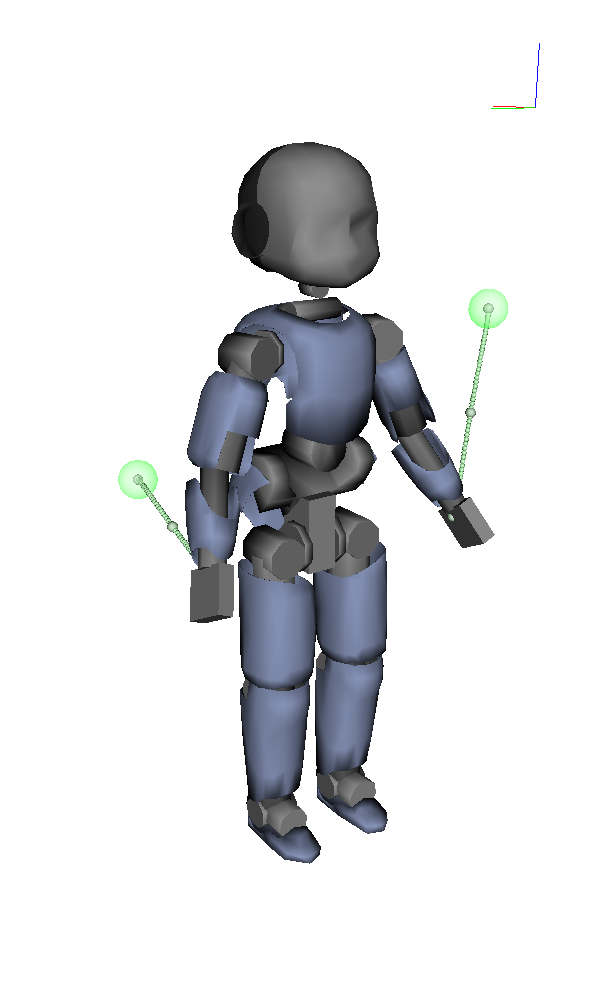
\includegraphics[trim = 0cm 4.5cm 0cm 5cm, clip, height=4 cm]{./sections/WP4/pics_UPMC/01_starting}
 \caption{Constrained Configuration}
 \label{fig:config}
\end{subfigure}
%
\begin{subfigure}{.31\linewidth}
 \centering
 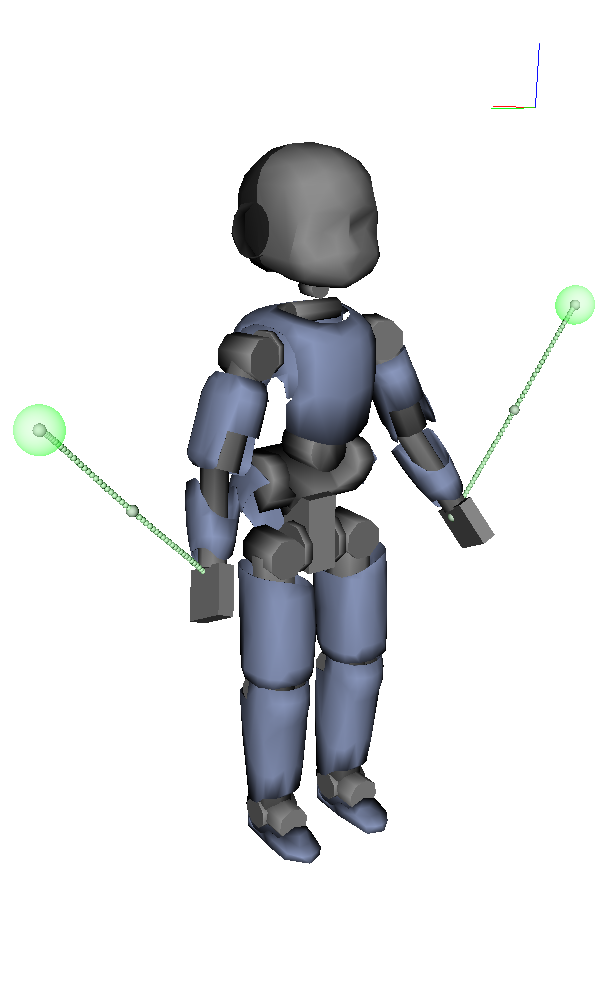
\includegraphics[trim = 0cm 4.5cm 0cm 5cm, clip, height=4 cm]{./sections/WP4/pics_UPMC/02_starting}
 \caption{Workspace Violation}
 \label{fig:work}
\end{subfigure}
%
\begin{subfigure}{.31\linewidth}
 \centering
 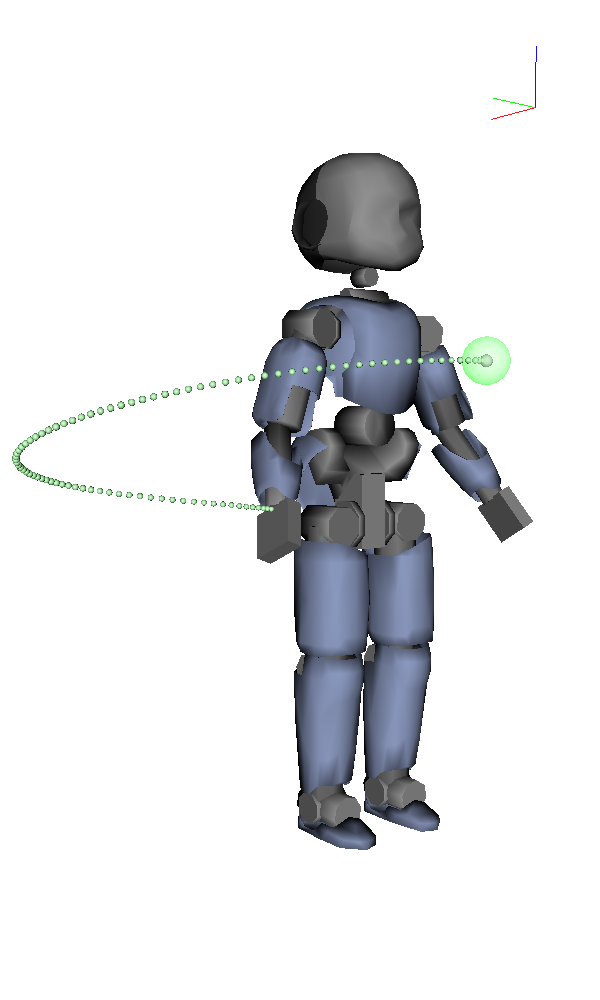
\includegraphics[trim = 0cm 5cm 0cm 5cm, clip, height=4 cm]{./sections/WP4/pics_UPMC/03_starting}
 \caption{Balance Perturbation}
 \label{fig:balance}
\end{subfigure}
%
\caption{Three common multi-task incompatibility scenarios. The desired hand
task trajectories are indicated by the green markers. Medium size spheres
represent waypoints, and large transparent spheres represent the final waypoints
or goals.}
\label{fig:3_scenarios_lober_2015}
\end{figure}


In a second study \cite{loberIROS2015}, we studied how task
variability can be used to modulate task priorities during their execution, to
temporarily deviate certain tasks in the presence of incompatibilities. A method
for mapping from task variance to task priority was presented as well as an
approach for calculating task variance for generated trajectories. The method
successfully resolved three common task conflict scenarios online illustrated on
Figure~\ref{fig:3_scenarios_lober_2015}.\\

%Valerio's paper on learning activation policies in task controller.
We also addressed the problem of learning the temporal profile of soft
task priorities and null-space projectors for the multi-task controllers
developed in \cite{liuGHC2015}.

The \textit{Prioritized Task-Space Inverse Dynamics} controller from \cite{DelPrete-2014-ID267}
is based on \textit{strict task hierarchies}, where a hierarchical ordering of
the tasks is set, such that critical tasks (or tasks that are considered as more
important) are fulfilled with higher priorities, and the low-priority tasks are
solved in the null-space of the higher priority tasks. The strict control approach requires the
pre-specification of the task hierarchy. However, in many contexts it is
difficult to organize the tasks in a stack and define their relative importance
in forms of priorities. When priorities are strict, a higher task can completely
block lower tasks, which can result in movements that are not satisfactory for
the robot mission (\textit{e.g.}, its ``global'' task). Swapping tasks can result in discontinuities of the control law.
Moreover, the task priority must be defined \textit{a priori}, which
is typically done by an expert able to define the tasks and their relative priorities to produce smooth behaviors.

Another set of whole-body controllers is based on \textit{soft task hierarchies}, where
the solution is typically given by a combination of weighted tasks (see for example \cite{Salini-2011-ID348}). 
The importance or ``soft priority'' of each individual
task is represented by a scalar function, often named ``weight''. By tuning the vector of scalar weights,
evolving in time, the global robot behaviour can be optimised. Liu et
al. \cite{liuGHC2015} propose a generalised projector (GHC) that handles
strict and non-strict priorities with smooth transitions when tasks priorities
are swapped. They show that adapting these weights may result in a seamless
transition between tasks (\textit{i.e.}, reaching for an object, staying close to a
resting posture and avoiding an obstacle) and in continuous task sequencing.
Despite the elegant framework, their controller needs again a lot of manual
tuning: particularly, the evolution of the tasks priorities in time, the timing
and the tasks transitions need to be designed by hand. While this approach could
still be easy for few tasks and simple robotic arms, it can quickly become
unfeasible for complex robots such as humanoids performing whole-body movements
that usually require multiple tasks and constraints (\textit{e.g.}, control balance,
posture, end-effectors, stabilise head gaze, prevent slipping, control
interaction forces etc.).

\begin{figure}%[t!]
\centering
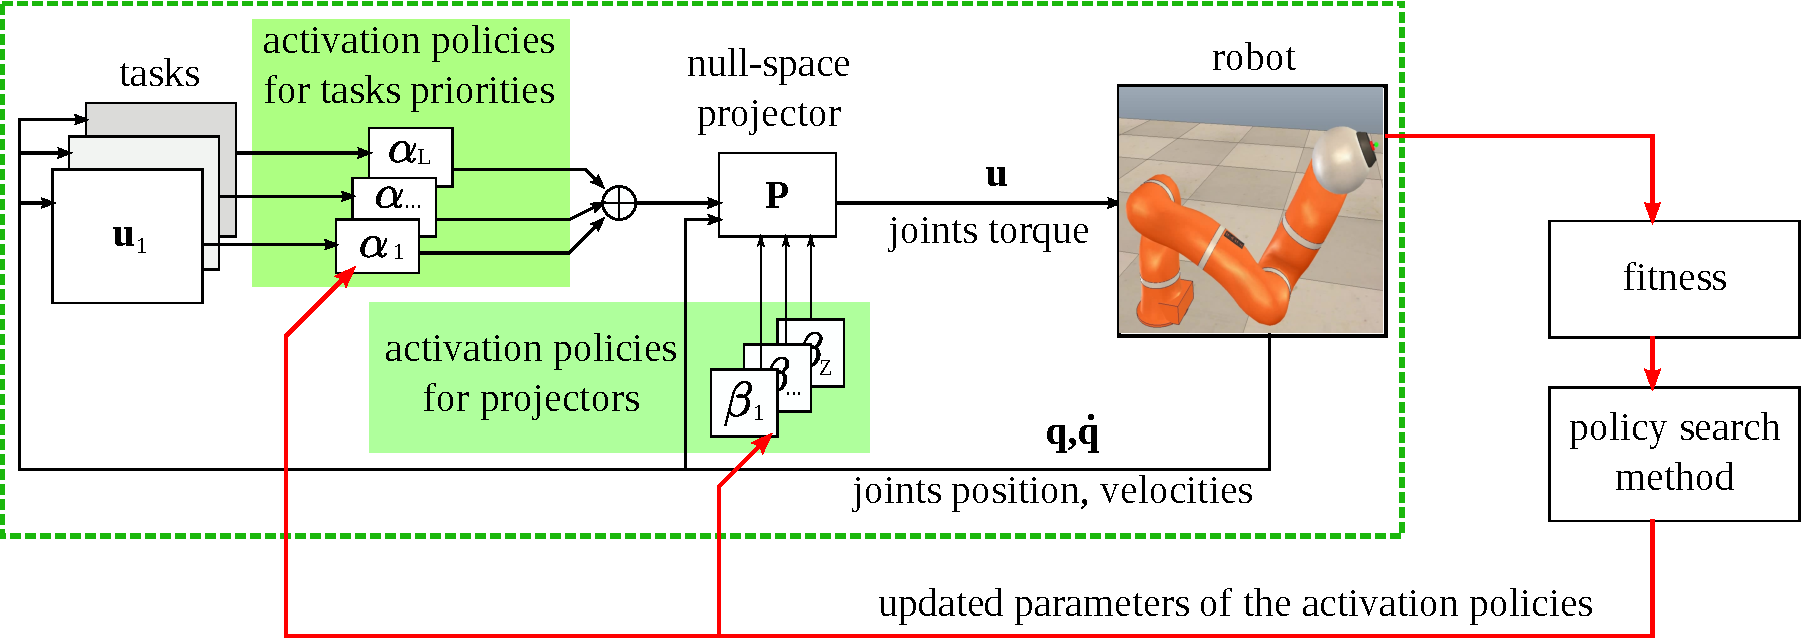
\includegraphics[width=\linewidth]{./sections/WP4/pics_serena/concept_scheme}
\caption{This scheme briefly describes the proposed method. The control torques are computed by a combination of tasks weighted by soft priorities, represented as parameterized activation policies, that are multiplied by a Null-space projector, where some activation functions for different projectors are joined. The global task execution is evaluated and a fitness function is computed: a policy search method is then used to optimize the parameters of the activation policies, both for tasks and projector. }
\label{figure:scheme}
\end{figure}

An intuitive solution to the problem of defining the weights is to learn or optimize them through trial-and-error. 
We study how the \textit{temporal} profiles of the task weights can be learned from a reward function, which is assumed to
be given\footnote{For many robotic task, \textit{e.g.}, tracking desired center-of-mass
or end-effector trajectories while avoiding obstacles, such reward functions
have been defined in \cite{Kober_IJRR_2013}.}. 
As a learning algorithm, we choose CMA-ES \cite{Hansen-2001-ID362}, a stochastic optimization derivative-free algorithm that is suitable for the optimization of non-linear and non-convex objective functions. The main reason for using CMA-ES is that it is relatively simple to use and with a small number of free parameters. However, any other optimization algorithm with similar properties could be used.
As a first step towards a controller that is capable of handling multiple tasks
and constraints on a complex robot, while allowing us to efficiently learn the
task priorities, we propose a regularized version of the Unified Framework (RUF)
proposed by Peters et al \cite{Peters_AR_2008}, where the tasks weights and
Null space projectors weights are represented by parametrized functional
approximators that can be automatically determined through a stochastic
optimization procedure. The concept is presented in Figure~\ref{figure:scheme}.

\begin{figure}%[b!]

\begin{subfigure}{.3\linewidth}
  \centering
  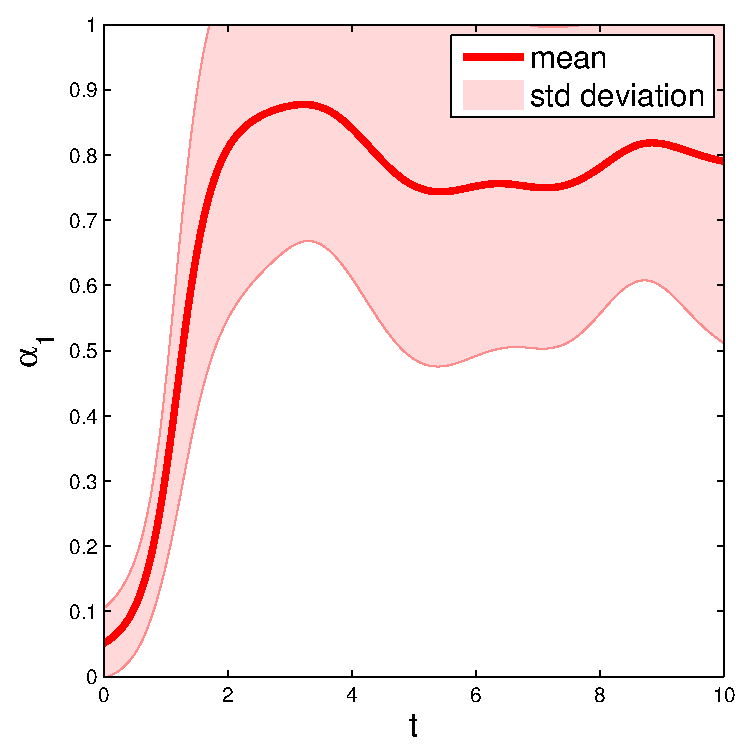
\includegraphics[width=\linewidth]{./sections/WP4/pics_serena/alpha1}
  \label{fig:alpha1}
  \caption{Attractor activation.}
\end{subfigure}%
\begin{subfigure}{.3\linewidth}
  \centering
  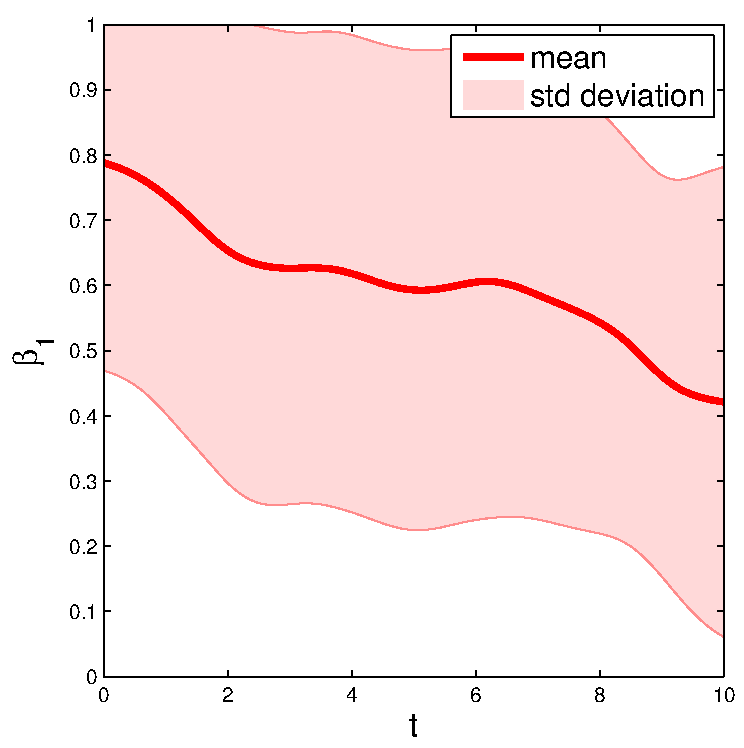
\includegraphics[width=\linewidth]{./sections/WP4/pics_serena/alpha2}
  \label{fig:alpha2}
  \caption{Null-projector activation.}
\end{subfigure}
\begin{subfigure}{.3\linewidth}
  \centering
  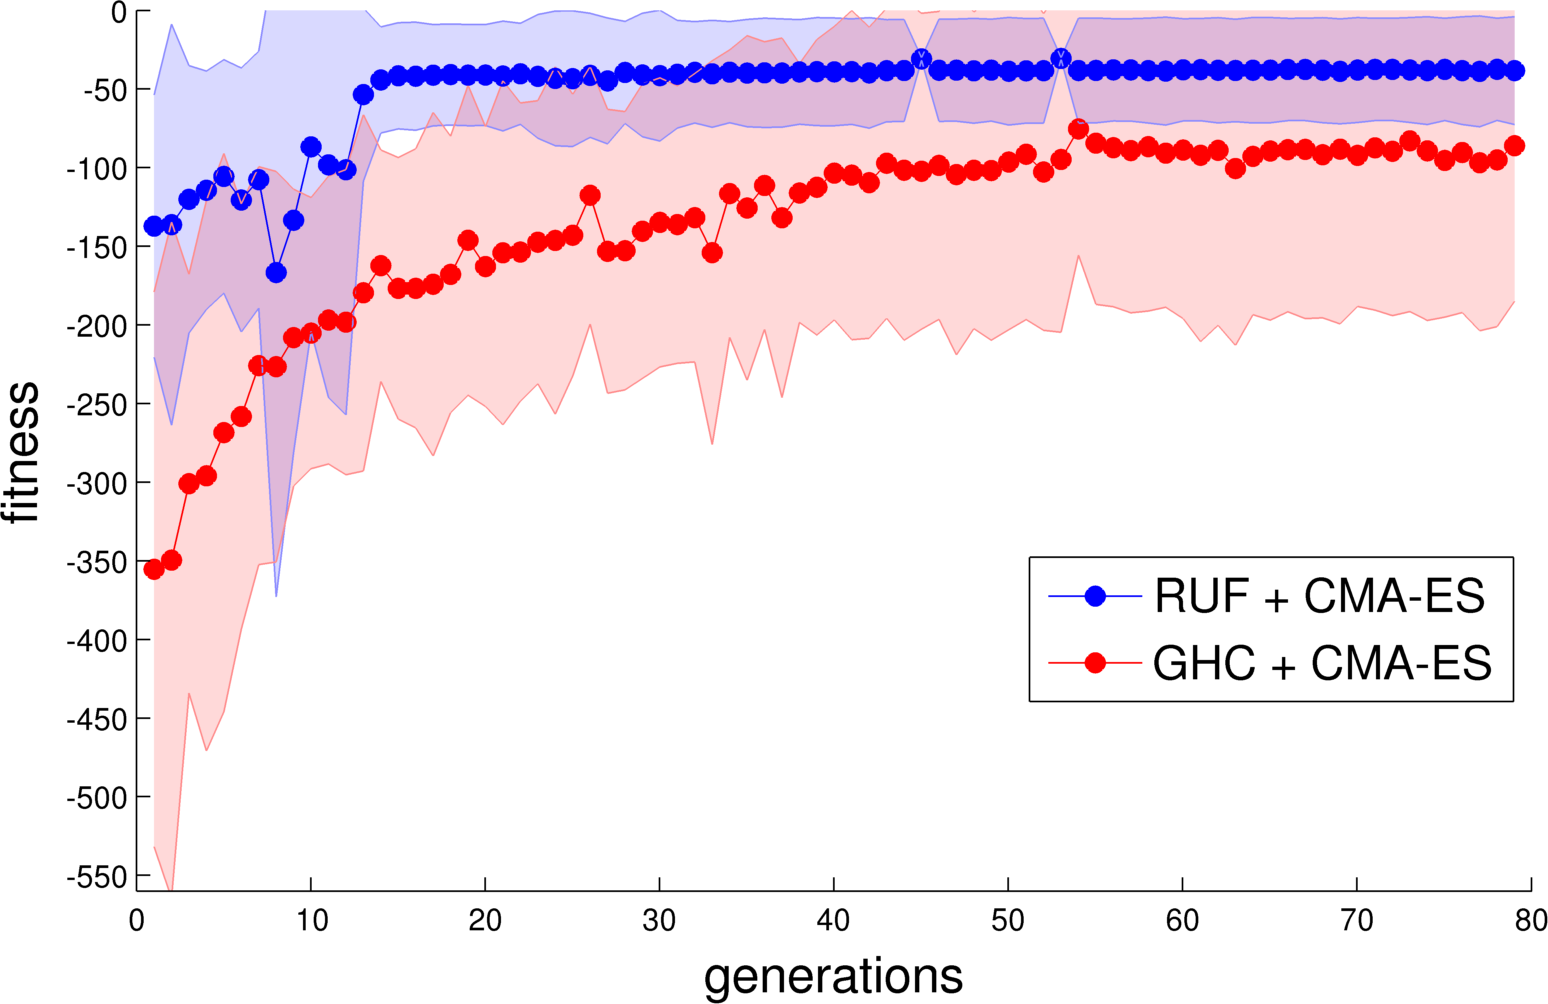
\includegraphics[width=\linewidth]{./sections/WP4/pics_serena/comparison}
  \label{fig:alpha3}
  \caption{Learning performance.}
\end{subfigure}
\caption{The panels in (a) and (b) show the mean and standard deviation of the temporal
profile of the activation functions $\alpha,\beta$, optimized by RUF+CMA-ES,
computed over $R=50$ replications of the same experiment of the table scenario.
(c) Comparison of our method (blue line) to the generalized projector method (GHC).}
\label{fig:activation_policy}
\end{figure}

As a first results, we show that the optimization process  generates weights
profiles that cannot be designed manually in advance, see panels (a) and (b) in 
Figure~\ref{fig:activation_policy}.

% \begin{figure}%[b!]
% \centering
% 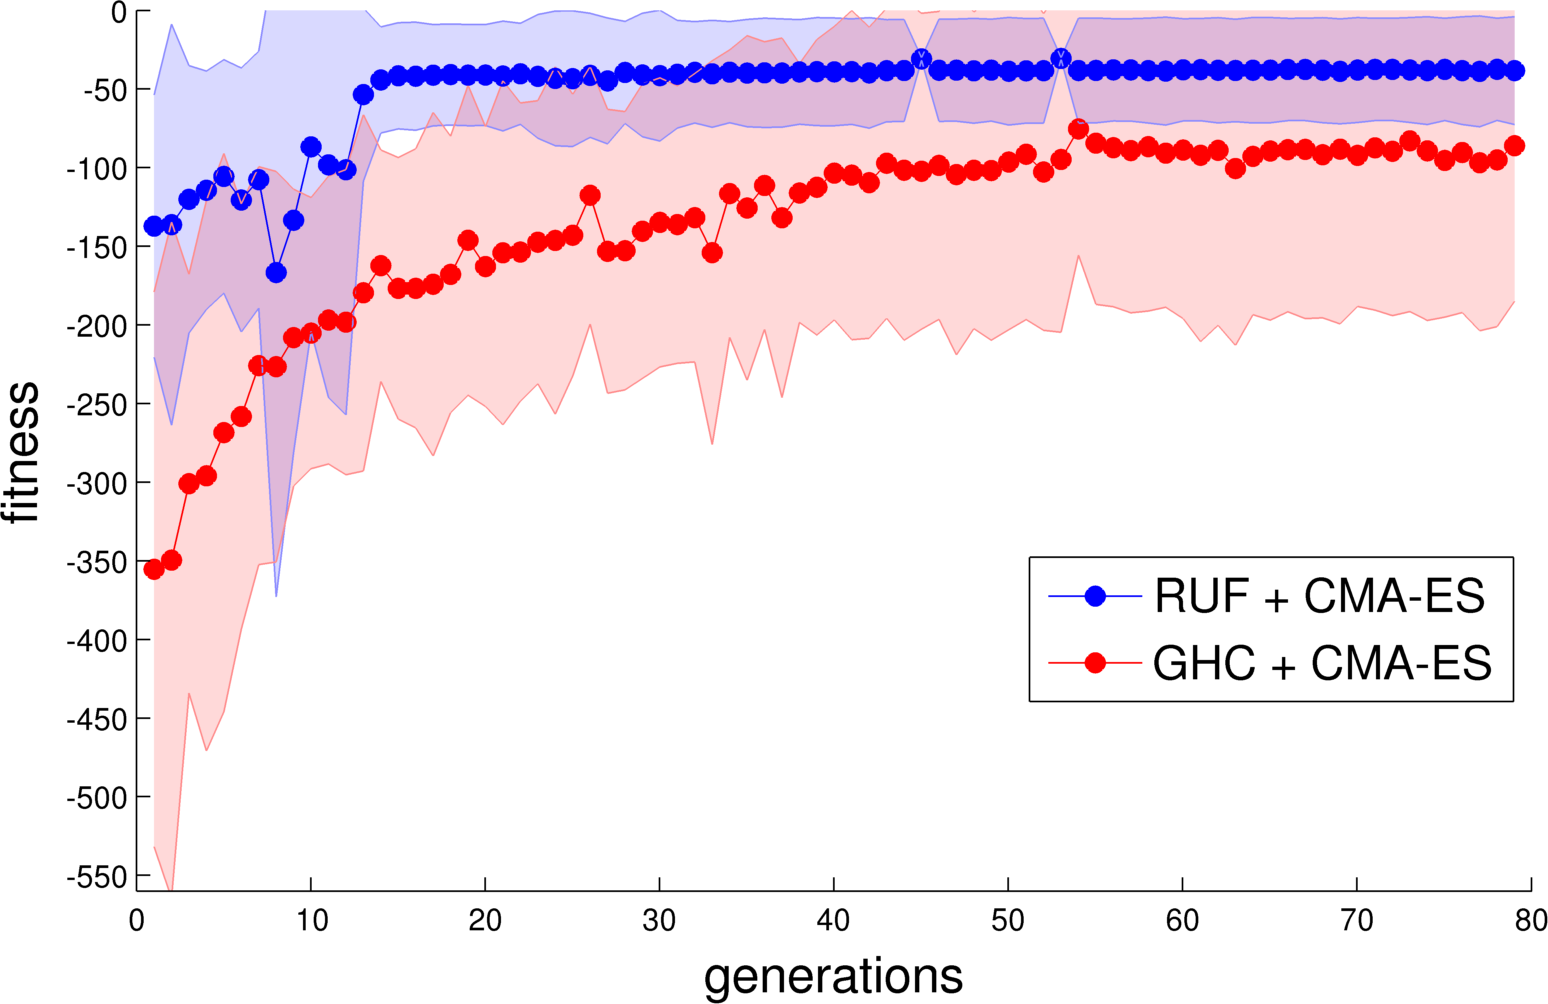
\includegraphics[width=1\hsize]{./sections/WP4/pics_serena/comparison}
% \caption{This figure shows the mean and the standard deviation of $R=20$
% replications of the same experiments for our method RUF+CMA-ES and GHC+CMA-ES.
% For both controllers, we consider a random initial point in the parameter space
% for the optimization algorithm. Our method shows a faster convergence learning
% rate and it reaches a better result in terms of the optimized fitness.}
% \label{fig:comparison}
% \end{figure}

We then compare the performance of our controller with the state-of-the-art
method GHC proposed by Liu et al. \cite{liuGHC2015}. We consider the
following experimental scenario: a 7-DOF KUKA Light Weight Robot arm, starting
from a vertical position, must reach a desired point with its end-effector,
while avoiding to collide with a table, represented by a surface parallel to the
z-axis in between the robot and the goal. The aim of the experiment is to bring
the end-effector as close as possible to the desired position, while avoiding
collisions with the obstacle. We define  $T=3$ tasks: a regulation task in the
joint space, and two reaching tasks for the elbow and the end-effector. For both
methods, we find the optimal profiles for the weighting functions with CMA-ES.
Our second result is that our controller generally performs better than GHC,
even if we optimize the policies in both methods: on an average of 20
replicates, our RUF+CMA-ES finds 90\% of the solutions found by our RUF+CMA-ES
satisfies the constraints, while only 75\% of the solutions of GHC+learning are
acceptable. Furthermore, the final best solution found by RUF+CMA-ES outperforms
the one of GHC+CMA-ES, as shown in Figure~\ref{fig:activation_policy} (c).



%This paper presents the control framework implemented on the humanoid robot iCub for one foot balancing and motion control.
%This framework ensures a degree of compliance for the multi-body system, which allows for safe human robot interaction.
%  and integration of all the building blocks composing a
% system for balance and motion control of a humanoid robot. The system includes the low-level joint-torque control,
% the task-space inverse-dynamics control, the task planner and the estimation of contact forces and joint torques.
% Even though in recent years other similar systems have been presented \cite{Ott2011, Herzoga},
% the originality of our contribution lies i) in the specificities of our test platform and ii) in a number
% of design choices that traded off simplicity of implementation for performances of the control system.
% In particular:
%  \begin{itemize}
% \item differently from the other robots, iCub can localize and estimate contact forces on its whole body thanks to its distributed tactile sensors
% \item similarly to the \emph{DLR-Biped} \cite{Ott2011}, iCub is actuated with DC motors and harmonic drives, but we chose to neglect the gear-box flexibility, which simplified the motor-identification procedure and the low-level torque controller
% \item differently from the above-mentioned platforms, iCub is not equipped with joint-torque sensors, but we designed a method that exploits its internal 6-axis force/torque sensors to estimate the joint torques
% \item all our control loops run at 100 Hz, which is (at least) 10 times slower with respect to \cite{Ott2011, Herzoga}
% \end{itemize}
% We believe that further investigation will be necessary to thoroughly understand all the consequences of our hardware/software design choices.
% Nonetheless, these peculiarities make the presented system unique, % in terms of both capabilities and simplicity of implementation,
% and for this reason we think it is important to share our results with the robotics community.


%The present paper discusses the theory and implementation of a controller for whole-body stability on
%multiple rigid noncoplanar contacts. The stability problem is reformulated as a contact-force control problem,
%which is solved exploiting recent results by \cite{DelPrete2014}. The theoretical framework is
%implemented on the iCub humanoid, an ideal robot for the specific implementation, \replaced[id=jeg, remark='in consideration of' is mostly used to express gratitude. Equivalent to  'in return for']{if you take into consideration its}{in consideration of its}
%whole-body distributed force and tactile sensing. The specificity of the platform calls for a number of custom
%choices\added[id=jeg, remark=Is this 'specificity' recalled as a disadvantage or negative aspect of the proposed controller anywhere in the paper?]{} discussed throughout the paper, which is organized as follows.

%\section{Validation scenarios}
%
%This section presents the control framework implemented on the humanoid robot iCub for one foot balancing and motion control. This framework ensures a degree of compliance for the multi-body system, which allows for safe human robot interaction.
%
%\subsection{System modelling}
%The system dynamics are characterized by the following  differential equations:
%
%\begin{eqnarray}\label{eq:dyn}
%\label{eq:dynNoContacts}
%M(q) \dot{\nu} + h(q, \nu) - J^\top(q) f  &=&
%{S} \tau \mbox{,}\\
%\label{eq:contact}
% J(q) \dot{\nu} + \dot{J}(q, \nu) \nu &=& 0 \mbox{,}
% \end{eqnarray}
%
%\noindent
%where $q \in SE(3) \times \Rv{n}$ represents the configuration of the free floating system,
% which is given by the
%pose of a base-frame and $n$ generalized coordinates $q_j$ characterizing the joint angles.
%% (includes both $q_j \in \Rv{n}$ and the
%% floating-base
%The vector $\nu \in \Rv{n+6}$ represents the robot velocity
%(it includes both $\dot{q}_j \in \Rv{n}$ and the linear and angular velocity of the base-frame $v_b \in \Rv{6}$), the system acceleration is denoted as $\dot \nu$,
%the derivative of $\nu$, the control input
%$\tau \in \Rv{n}$ is the vector of joint torques, $M \in \R{(n+6)}{(n+6)}$ is the mass matrix, $h \in \Rv{n+6}$ contains both
%gravitational and Coriolis terms, $S \in \R{n}{(n+6)} := (0_{n\times 6}, I_n)^\top$ is the matrix selecting the actuated degrees of freedom, $k$ is the number of constraints acting on the system, $f \in \Rv{k}$ are the generalised forces associated to the constraints, and $J \in \R{k}{(n+6)}$ is the constraint Jacobian \eqref{eq:contact}.
%
%
%\subsection{Problem statement}
%
%The control objective is the asymptotic stabilization of a desired centroidal dynamics \cite{Orin2013}. Let $H$
%denote the centroidal momentum of the robot. Then, the time derivative of $H$ is equal to the summation of the external wrenches acting on the multi-body system. By expressing the centroidal momentum with respect to the center of mass, we have:
%
%\begin{eqnarray} 
%    {\dot H}  =   X f + mg 
%     = \begin{pmatrix} m \ddot{x} \\ \dot{H}_\omega  \end{pmatrix} \label{eq:constraintsSi}
%\end{eqnarray}
%where $m$ is the mass of the robot, $g \in \mathbb{R}^6$ is the gravitational acceleration, $\ddot{x} \in \mathbb{R}^3 $ 
%is the acceleration of the center of mass, $H_\omega \in \mathbb{R}^3$ is the \emph{angular momentum} of the robot, and the matrix $X$ maps the contact wrenches on the center of mass.
%
%The control objective is to find a control law for the inputs $\tau$ such that $x \rightarrow x(0)$ and $H_\omega \rightarrow 0$. This choice is sufficient for balancing purposes. Also, while achieving this control objective, the system shall have a degree of compliance.
%
%\subsection{The control strategy}
%The control strategy is composed of two steps. We first choose the external force $f$ such that $x \rightarrow x(0)$ and $H_\omega \rightarrow 0$. Then, we generate this force through the internal torques. Since iCub possesses more than six degrees-of-freedom, which are necessary to generate the contact force $f$, we choose the remaining control inputs so that to have compliance at the joint level.
%
%\subsection{The choice of the contact force}
%
%Being the matrix $X$ invertible, the contact force $f$ achieving the control objective may be chosen as follows:
%
%\begin{multline} 
%    \label{fd}
%   f = -X^{\dagger}\left[k_d H + k_p\begin{pmatrix} x-x(0) \\ 0_{3\times1}  \end{pmatrix} + mg\right] \\ + \left( I - X^{\dagger} X \right) f_0, 
%\end{multline}
% with $k_d$ and $k_p$ two positive constants and $f_0$ arbitrarily chosen to obtain a solution $f$ as similar as possible to a desired value.
% 
% In order to keep the motion constraints satisfied, $f$ must satisfy some constraints, \textit{e.g.}, the contact forces
% must belong to the associated friction cones. In general, the contact constraints can be represented by inequalities of the 
% form $Cf < d$, with the matrix $C$ and the vector $d$ properly chosen. Then, we choose the contact wrench  as fallows:
%
%\begin{subequations} \label{eq:TSID}
%\begin{align}
%\label{eq:torquesTSID}
%  f = & \argmin_{  \xi \in \mathbb{R}^6} \|   \xi -   f_d\|^2 \\
%\label{eq:dynTSID}
%& \mbox{s.t.}  \quad C\xi < d, 
%%\label{eq:motionTSID}
%% J_i \ddot{  q} + \dot{J}_i \dot{  q} & = \ddot {  x}_i^*, \qquad i = 1, \dots, N -1
%\end{align}
%\end{subequations}
%with the desired wrench $f_d$ given by \eqref{fd}.
%
%%
%% \begin{eqnarray}
%%     {\dot H}  & = &   { X}^*_{lf} f + mg = \begin{pmatrix} m \ddot{x} \\ \dot{H}_\omega  \end{pmatrix} \label{eq:constraintsSi}
%%     % A & = & \begin{bmatrix} ^{com} { X}^*_{rf} & ^{com} { X}^*_{lf} \end{bmatrix}, \notag
%% \end{eqnarray}
%%
%% Let us briefly recall how the force-control problem is solved in the Task Space
%% Inverse Dynamics (TSID) framework
%% proposed by \cite{delPrete2013} in the context of free floating robots.
%% The framework computes the
%% joint torques to match as close as possible a desired vector of forces at the contacts \eqref{eq:torquesTSID}
%% while being compatible with the system dynamics \eqref{eq:dynTSID} and contact constraints
%% \eqref{eq:contactTSID}:
%%
%% \begin{subequations} \label{eq:TSID}
%% \begin{align}
%% \label{eq:torquesTSID}
%%   {\tau}^* = & \argmin_{  \tau \in \mathbb{R}^n} \|   f -   f^*\|^2 \\
%% \label{eq:dynTSID}
%% & \mbox{s.t.}  \quad M \dot{ \nu} + h - J^\top   f = S   \tau \\
%% \label{eq:contactTSID}
%% & \quad \quad J \dot{ \nu} + \dot{J}_c \nu  = 0
%% %\label{eq:motionTSID}
%% % J_i \ddot{  q} + \dot{J}_i \dot{  q} & = \ddot {  x}_i^*, \qquad i = 1, \dots, N -1
%% \end{align}
%% \end{subequations}
%% \noindent
%% where $f^* \in \Rv{k}$ is the desired value for the contact forces.
%% %${  x}^*_i (q)$ is  is the desired value for some kinematics variables ${  x}_i (q)$ and $J_i = \partial x_i / \partial q$ is the associated Jacobian.
%% Then we can exploit the null space of the force task to perform lower priority motion tasks.
%% These tasks (indexed with $i$) are all expressed as the problem of tracking a given reference acceleration $\dot {\nu}_i^*$ for a
%% variable ${x}_i$ differentially linked to $q$ by the Jacobian $J_i$.
%% We impose that the force task has maximum priority in the task hierarchy.
%% The final solution, i.e. the torques to be applied to the robot, are obtained by recursively solving a minimization problem similar to (\ref{eq:TSID}) in the null space of all the tasks with higher priorities.
%% Assuming that the force task has maximum priority the solution is:
%% \begin{equation} \label{eq:hyb_dyn}
%%   \tau^{*} = -(J\bar{S})^\top   f^* + N_j^{-1} {\dot{v}}_1^* + \bar{S}^\top n,
%% \end{equation}
%% where $N_j^{-1} = M_j - M_{bj} M_j^{-1} M_{bj}^\top$, $\bar S = \mat{-M_{bj}^\top M_b^{-1} & I}^\top $ and the term ${\dot{v}}_1^*$ is computed solving the following recursion for $i =N$, $\dots$, $1$:
%% \begin{equation}
%% \begin{split}
%% \dot{v}_i =& \dot{v}_{i+1} + (J_i \bar{S} N_{p(i)})^\dagger (\ddot{  x}_i^*-\dot{J}_i v + J_i (U^\top M_b^{-1} (h_b - J_{cb}^\top f) - \bar{S} \dot{v}_{i+1}))\\
%% N_{p(i)} =& N_{p(i+1)} - (J_{i+1} \bar{S} N_{p(i+1)})^\dagger J_{i+1} \bar{S} N_{p(i+1)}, \\
%% %N_{p(i)} =& I - \sum_{j=i+1}^{N}(J_j \bar{S} N_{p(j)})^+ J_j \bar{S} N_{p(j)},
%% \end{split}
%% \end{equation}
%% where $U \in \mathbb{R}^{6 \times (n+6)}$ is the matrix selecting the floating-base variables, and the algorithm is initialized setting $\dot{v}_{N+1} = 0$, \mbox{$N_{p(N)}=I$}, $J_N = J$ and $\ddot{ x}_N = 0$.
%% The implementation of this controller exploits the fact that we can compute \eqref{eq:hyb_dyn} with an efficient hybrid-dynamics algorithm.
%
%\subsection{The choice of the joint torques}
%The control input $\tau$ must generate the force $f$. The relationship between the contact wrench and the joint torques can be obtained by using the constraint equation along with the free-floating dynamics, i.e. Eq. \eqref{eq:dyn}.
%One can show that the torques generating $f$ are given by the summation of two terms, i.e.,
%\begin{eqnarray}
%        \label{tau}
%        \tau = \tau_f + N \tau_0,
%\end{eqnarray}
%where $\tau_f $ ensures $f = f_d$, the matrix $N \in \mathbb{R}^{n\times n}$ is the null space projector of 
%$JM^{-1}S$,
%and $\tau_0$ is a vector that can be chosen at will. To obtain compliance at joint level, we choose $\tau_0$ similar to 
%a gravity and external force compensation, plus a term of the form \[ -k(q_j - q_d),\]
%which ensures  compliance at joint level.
%
%
%% The control framework described in the previous section can be applied for a balancing task, while retaining the possibility of interaction with the environment.
%% Instantaneous values for interaction forces at feet are computed to
%% follow a prescribed center-of-mass trajectory ($x_{com}^d$) and to reduce angular momentum\footnote{Quantities are defined with a notation similar to \cite{Featherstone2008}}. A reference value  $\dot H_{com}^*$ for the total rate of change of spatial momentum (expressed at the center of mass) is computed as:
%%
%% \begin{eqnarray} \label{eq:hRef}
%% {\dot H}^* (t) = {\dot H}_{com}^d (t) -  K_d^{h} \tilde{H}_{com} - \begin{bmatrix} K_p^{com} \left( \tilde{x}_{com} \right)\\ 0_{3\times1}  \end{bmatrix}
%% \end{eqnarray}
%%
%% \noindent
%% where $K_d^{h}$, $K_p^{com}$ are suitably defined gain matrices, $\tilde{(\cdot)}$ denotes the error with respect to the desired quantity, $H_{com}$  and $H_{com}^d = [m \dot{x}_{com}^{d\top}, 0_{1\times3}]^\top$ is the spatial momentum around the center of mass and its desired value, $x_{com}$ is the center-of-mass cartesian position, $x^d_{com}$ its desired value and $m$ is the total mass of the robot.
%% The relation between external forces and ${\dot H_{com}}$ is given by the following equation:
%% % At this point $f^*$ can be computed from ${\dot H_{com}}^*$
%% % considering that the time derivative of the momentum equals the resultant of forces and torques if all
%% % quantities are computed with respect to the center of mass:
%% \begin{eqnarray}
%%     {\dot H_{com}}  & = &   A f + f_g \label{eq:constraintsSi}\\
%%     A & = & \begin{bmatrix} ^{com} { X}^*_{rf} & ^{com} { X}^*_{lf} \end{bmatrix}, \notag
%% \end{eqnarray}
%% where $f_g$ is the gravitational force and where the matrices $^{com} { X}^*_{(\cdot)}$  express the spatial forces acting on the left foot ($lf$) and right foot ($rf$) with respect to the center of mass.
%% In literature these equations (derived from the Newton-Euler equations) have been presented in detail by
%% \cite{Orin2013} under the name of \emph{centroidal dynamics}.
%%
%% Finally, the desired force $f^*$ can be computed as
%%
%% \begin{equation} \label{eq:minF}
%%  f^* = \argmin_{f} \|  f  - f_0 \|^2  \qquad \mbox{s.t.} \qquad A f + f_g = {\dot H_{com}}^*,
%% \end{equation}
%% The solution of this optimization is given by:
%% \begin{equation}
%%  f^* = A^{\dagger} \left( {\dot H_{com}}^* - f_g \right) + (I - A^{\dagger} A)  f_0 ,
%% \end{equation}
%% \noindent
%% where $f_0$ can be chosen to satisfy additional constraints on the forces.
%%
%% We also added, at the lowest priority level, a postural task. Reference accelerations for the joint variables are chosen as:
%%
%% \begin{equation} \label{eq:qRef}
%% {\ddot q_j}^* (t) = {\ddot q_j}^d (t) - K_d^{q} \left( {\dot q_j} - {\dot q_j}^d (t) \right) - K_p^{q} \left( {q_j} - { q_j}^d (t) \right),
%% \end{equation}
%% where $K_p^{q}$ and $K_d^{q}$ are arbitrary positive-definite matrices
%% This task acts in the null space of the task force as specified in Eq. (\ref{eq:TSID}).
%% In the general case more tasks can be added between the highest priority one (force task) and the lowest priority one (postural task).
%
%\subsection{Experiment}
%
%\begin{figure}
%\centering
%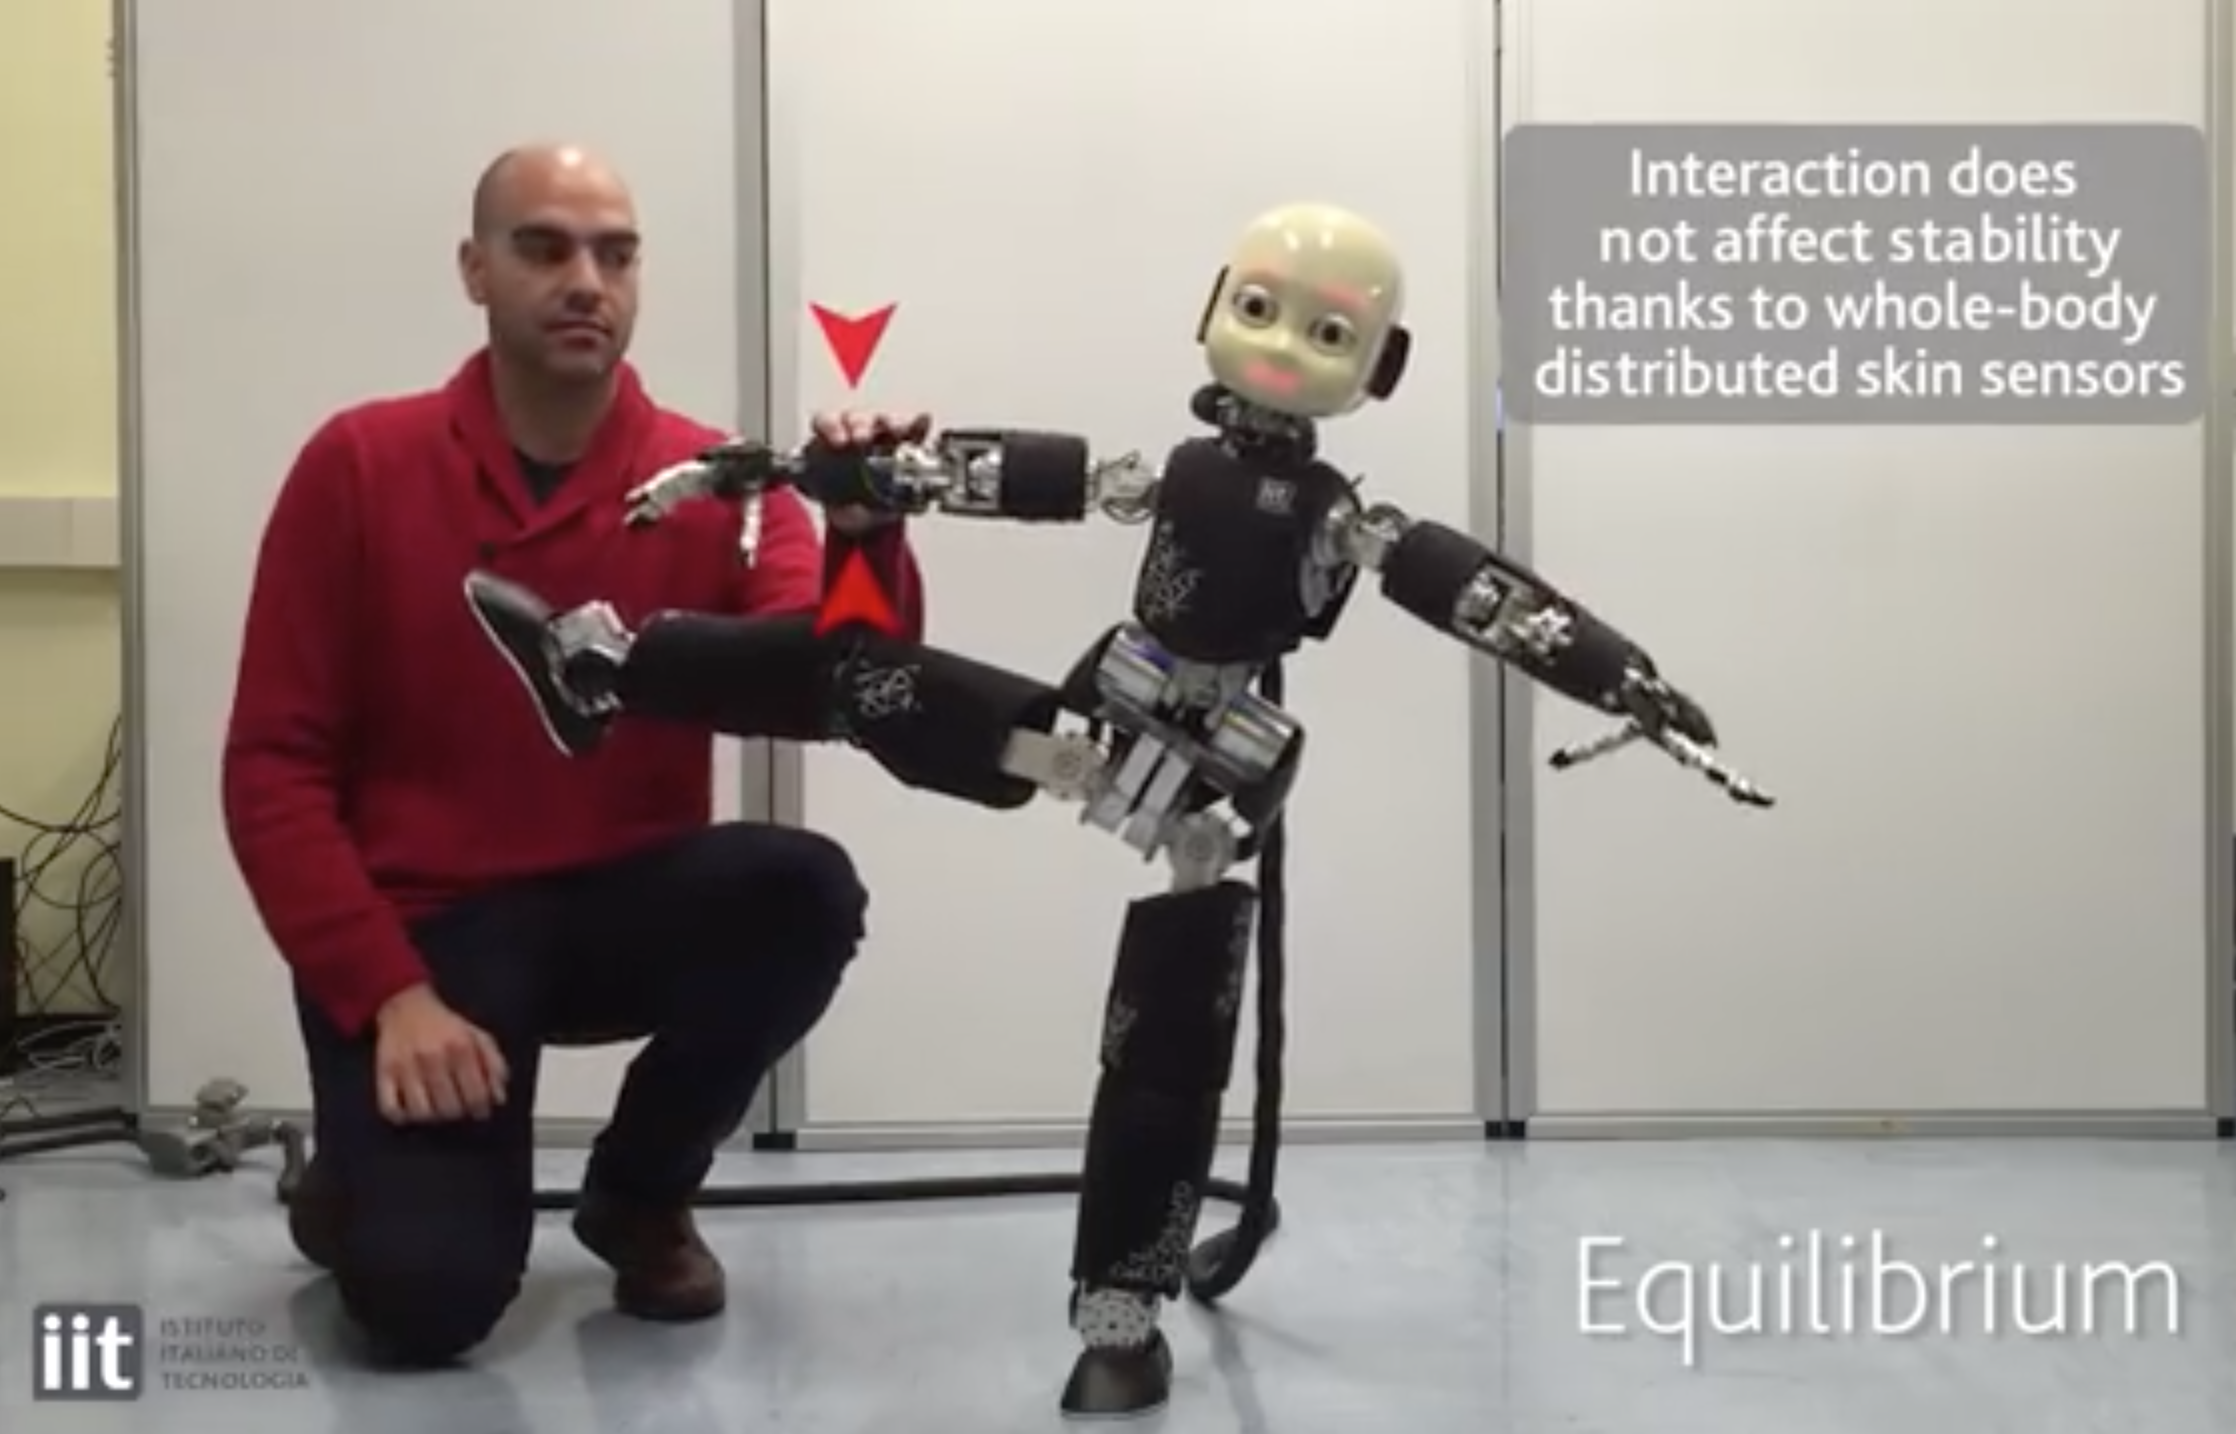
\includegraphics[width=0.9\columnwidth]{images/icubPicture} \\
%\caption{Screenshot of the video showing the full experiment. iCub balances by controlling the foot wrench.
%} \label{fig:snapshot}
%\end{figure}
%
%% \begin{figure}
%% \centering
%% \includegraphics[width=0.8 \textwidth]{images/twoSupportsSignals.pdf} \\
%% \caption{Results of the double support experiment on planar contacts (left and right feet). The picture shows
%% the time behavior of forces (top) and center of mass position (bottom) on the sagittal (blue) and transverse
%% (green) axis. It is worth \replaced[id=jeg]{noting}{noticing} that forces should be proportional to center of mass accelerations and this
%% is visible in the plot considering that accelerations are \replaced[id=jeg]{sinusoidal}{sinusoid} in counter phase with positions.
%% \adnote{Add desired CoM trajectory and desired forces?} Rapid variations of the contact forces at the time $t \approx 2$, i.e. starting time, are due to
%% the activation of the torque control.}
%% \label{fig:twoSupportsForces}
%% \end{figure}
%%
%% \begin{figure}
%% \centering
%% \includegraphics[width=0.4 \textwidth]{images/twoSupports.pdf}
%% \includegraphics[width=0.4 \textwidth]{images/twoSupportsFRI.pdf}
%% \caption{Results of the double support experiment on planar contacts (left and right feet). The left picture
%% shows in three dimensions the feet contacts, the feet center of pressures, the forces at the feet and at the
%% the center of mass during three instants: at two extrema of the sinusoid (red and blue) and in the middle of
%% the sinusoid (green). Remarkably forces are maximum at the extrema when also accelerations are
%% maximal. The right picture shows a close-up of of the feet with the trajectory of the center of pressure, an
%% ellipse representing a Gaussian fit of the data points and three points corresponding to the position of the
%% centers of pressure when at the two extrema of the sinusoid (red and blue) and in the middle of the sinusoid
%% (green). \adnote{I found this figure hard to interpret, even after reading the caption, the RGB arrows/points are hard to see.}} \label{fig:twoSupports}
%% \end{figure}
%%
%% \begin{figure}
%% \centering
%% 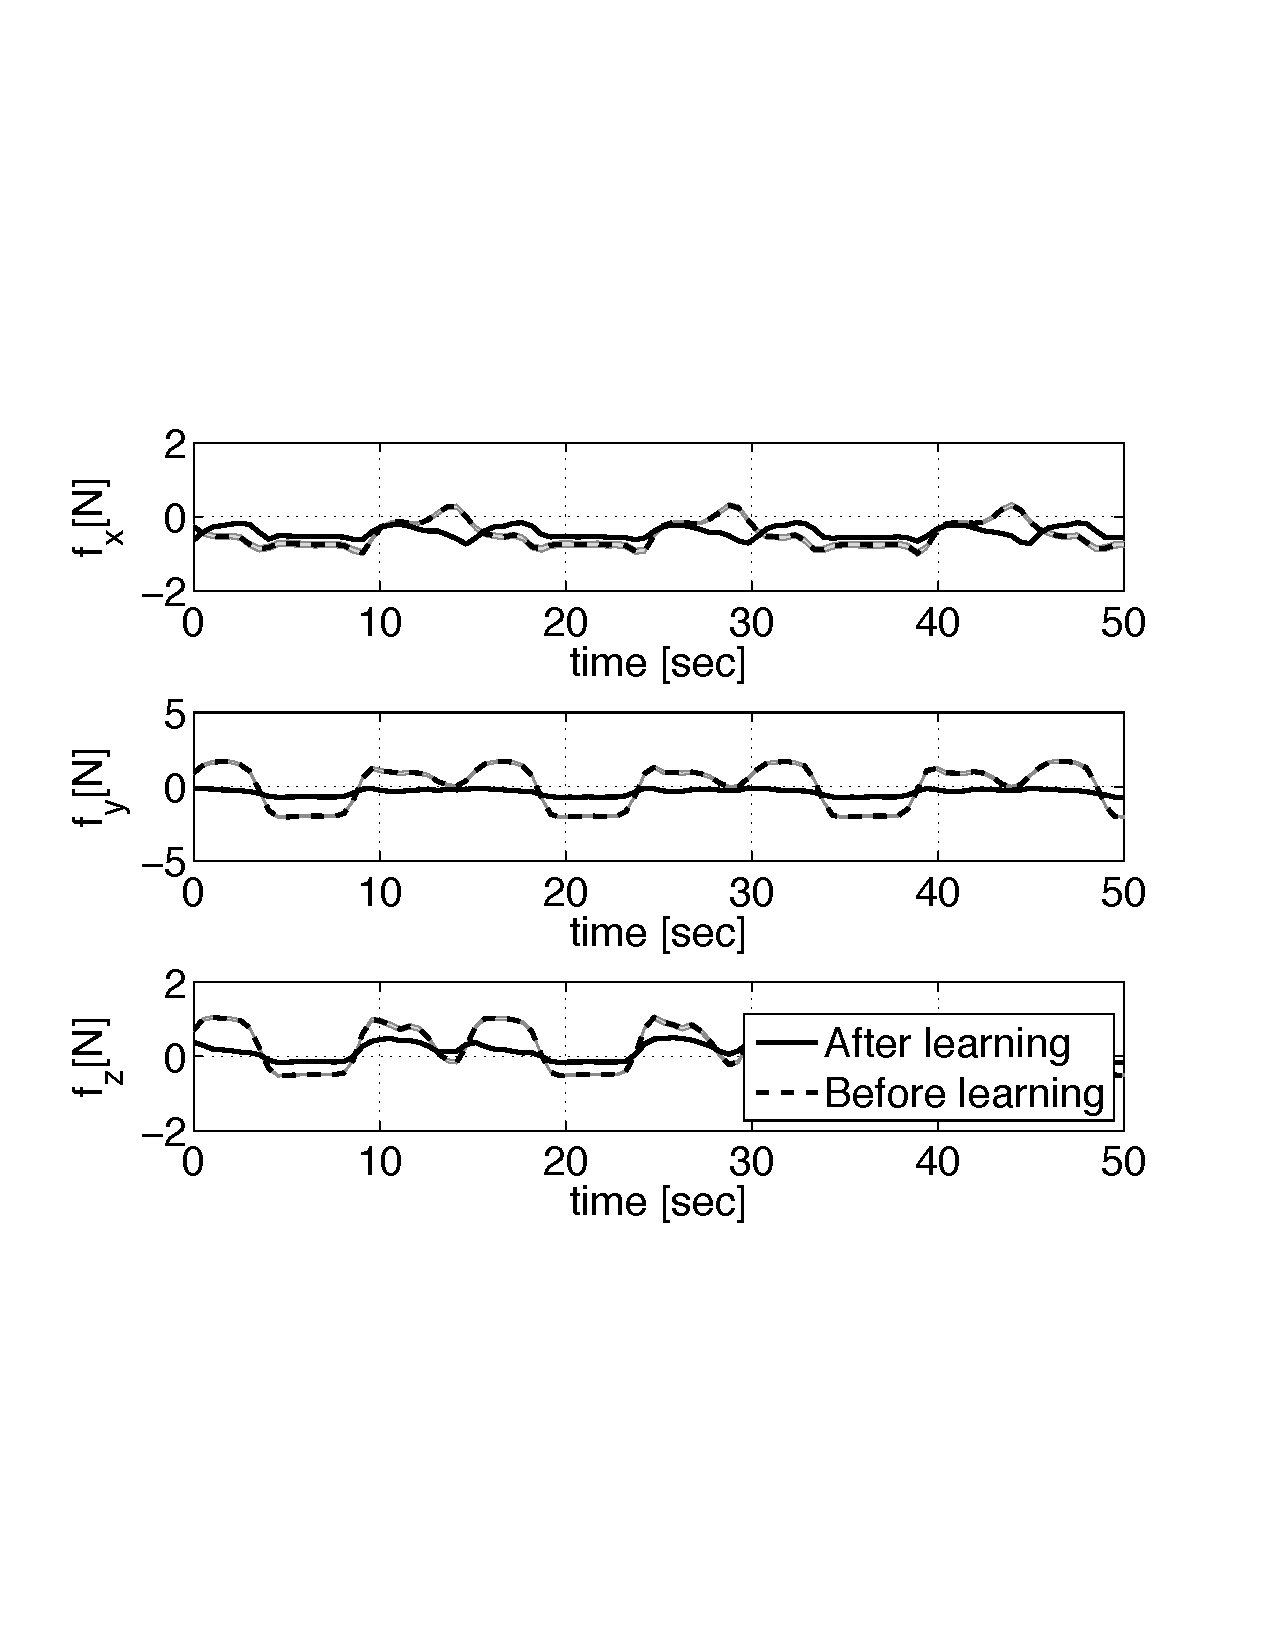
\includegraphics[width=0.8 \textwidth]{images/forces.pdf} \\
%% \caption{Results of the double support experiment on four noncoplanar contacts (both feet and
%% arms). The plots represent the evolution of the contact forces at the left (top) and right (bottom) arms when
%% contact is established.} \label{fig:fourSupportsForces}
%% \end{figure}
%%
%% \begin{figure}
%% \centering
%% \includegraphics[width=0.4 \textwidth]{images/fourSupports.pdf}
%% \includegraphics[width=0.4 \textwidth]{images/fourSupportsFRI.pdf}
%% \caption{Results of the double-support experiment on four noncoplanar contacts (both feet and
%% arms). The left picture gives a three-dimensional view of the foot center-of-pressure positions together with
%% the arm contact forces. Forces are represented in a color scale that goes from black (contact establishment)
%% to blue (steady state) \adnote{I found the forces hard to interpret so I'd remove them since they are already in the previous plot}.
%% The right picture gives a closeup on the foot center-of-pressure positions with an
%% ellipse that represents the Gaussian approximation of its distribution. \adnote{Overall this figure is hard to read, so I suggest replacing
%% it with a plot of the CoP.}} \label{fig:fourSupports}
%% \end{figure}
%
%We implemented the proposed control strategy on the iCub platform as illustrated in Figure~\ref{fig:snapshot}. The control framework is composed of two
%loops. The inner loop is in charge of stabilizing \emph{desired} joint torques, while the outer loop is governed by 
%Eq. \eqref{tau}. Both loops runs at the same frequency of 100 Hz. 
%
%The experiment consists in two phases. In the first phase, we change the desired $q_d$ in order to generate 
%\emph{internal} motions, which do not perturb the stability of the robot momentum thanks to the prioritization of tasks
%described in the previous section. In the second phase, we apply external perturbations by interacting with the robot as illustrated in Figure~\ref{fig:footBalancing}. This 
%interaction  results to be safe thanks to the compliance at joint level\footnote{A video of the experiment is available \href{https://www.youtube.com/watch?v=VrPBSSQEr3A}{\textbf{here}} for the interested reader.}.
%
%For more detailed information and description of the system architecture (comprising torque and forces estimation and low level torque control) see \cite{noriFrontiers2015}.

\section{Conclusions}

In this paper we report on the current state-of-the-art in whole-body dynamics studies concerning human movement analysis, robot control and learning. We outline a roadmap of experiments  and  research  questions  that  are  currently  explored  by  the  consortium  of the European Project CoDyCo.

We also briefly present some of the recent CoDyCo advances in these domains. These numerous intertwined contributions cover four domains: control theory, machine learning, human behavioural experiments and software. They can be summarized as follows:
\begin{itemize}
\item Design, implementation and maintenance of a whole-body control software infrastructure. The infrastructure consists of several modules which significantly improve  controllers accuracy and robustness thanks to a module for whole-body torques estimation, a module for force/torque sensors calibration, a module for whole-body dynamics identification and a module for dynamics estimation.
\item Design of experimental protocols and data collection of experiments for studying humans in multi-contact interaction with the environment. This includes experiments on hand-contact assisted balancing for examining the functional role of supportive hand contact, a metric for whole-body stability characterisation,  experiments of human-robot physical interaction to study strategies of dealing with uncertainties in contact and a study on human contact choice learning through physical interaction.
\item Design and test of state of the art control strategies for whole-body motion with multiple contacts through the development of a solver for the whole-body reactive control that provides an expressive and rich description of the control problem as well as an efficient way of solving it.
\item Design and simulation of whole-body control strategies in presence of non-rigid contacts and experiments on postural control under multiple environmental contacts while controlling the operational space dynamics.
\item Development of a theoretical framework for representing movement primitives within probabilistic contexts.
\item Design of a model-free probabilistic representation for simultaneous representation of kinematic and force trajectories.
\item Preliminary studies on the problem of learning strategies to adapt temporal activation of low-level primitives and to deal with interferences in combining multiple whole-body tasks.
\item Implementation of a validation scenario consisting in whole-body motion control subject to postural, contact and goal-directed (Cartesian) constraints.
\end{itemize}

Future works will be focused on the two challenges defined in introduction. More specifically, we would like to show that the iCub is able to learn how to exploit compliant contacts during whole-body tasks. Suitable control actions will be learnt (either on-the-fly or after few trials) and adapted to the compliance of the perceived contact, to be learnt on-line and a-priori unspecified. 

We also aim at showing the iCub capability to successfully take advantage of the help of a naïve caregiver willing to give support in performing a task otherwise impossible to perform. Proper task execution will require a certain amount of training/learning (ideally boot-strapped using the findings of the human experiments), to be performed either off-line (i.e. prior to the demonstration) or on-line (i.e. during successive trials). The naive caregiver will be given a set of instructions to leave a natural degree of autonomy. The iCub will be in charge of properly tuning its own compliance flowing the caregiver intentions. The expected validation scenario will involve a caregiver helping the iCub to stand (either from the ground or from a chair).

These works and future works on dealing with compliant and unknown environments will provide significant advances in the understanding of the use of contacts both in human motor control and humanoid robot control.



\section{Acknowledgement}
This paper was supported by the FP7 EU projects CoDyCo (No. 600716 ICT 2011.2.1 Cognitive Systems and Robotics).

\section{References}
\bibliography{ias_bibliography,ias_state_of_art}
\bibliographystyle{plain}

\end{document}
%\endinput
%%
%% End of file `elsarticle-template-num.tex'.
